\documentclass{beamer}
\mode<presentation> {
  \usetheme{Madrid} % or try Darmstadt, Madrid, Warsaw, ...
  \usecolortheme{default} % or try albatross, beaver, crane, ...
  \usefonttheme{default}  % or try serif, structurebold, ...
  \setbeamertemplate{navigation symbols}{}
  \setbeamertemplate{caption}[numbered]
} 

\usepackage[english]{babel}
\usepackage[utf8x]{inputenc}
\usepackage{graphicx}
\usepackage{amsmath}
\usepackage{amsfonts}
\usepackage{amssymb}
\usepackage{hyperref}

\usepackage{import}
\usepackage{standalone}
\usepackage{wrapfig}

\usepackage{tikz}
\usepackage{subcaption}
\usetikzlibrary{calc}
\usetikzlibrary {shapes.geometric}

%Defines theorem enviroments
\theoremstyle{definition}


\title[The 17 Wallpaper Groups]{Frieze Groups, Lattices and Wallpaper groups}
\author{Braydon Xuereb, James Butcher, Rory Yarr}
\institute[University of Newcastle] % (optional)
{
  MATH3120 Abstract Algebra \\
  University of Newcastle
}
\date{4 June, 2024}

\begin{document}

\begin{frame}
  \titlepage
\end{frame}
\begin{frame}{Wallpaper groups}
    \begin{figure}
        \centering
        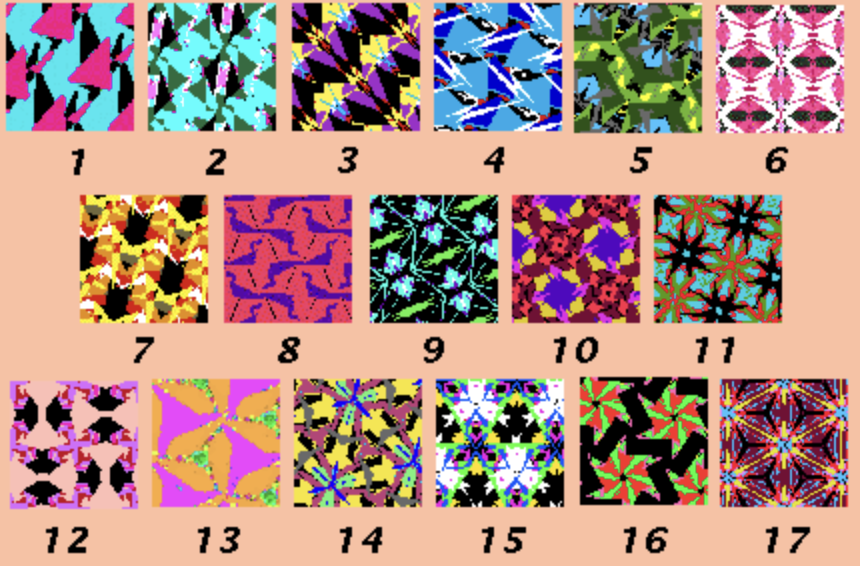
\includegraphics[width=0.9\textwidth]{Figures/WallpaperGroupsExample.png}
        \caption{The 17 wallpaper groups \cite{Clark1}}
        \label{fig:17WallpaperGroups}
    \end{figure}
\end{frame}

\begin{frame}
  \frametitle{Introduction, group operations}
  \begin{definition}[Types of Symmetries]
  \begin{itemize}
      \item Translations 
      \item Reflections
      \item Glide Reflections
      \item Rotations.
  \end{itemize}
  \end{definition}
\end{frame}



\begin{frame}{Translations }
\begin{definition}
     Translations are repetitions of a pattern structure.  defined mathematically as follows \\ 
    a mapping $t_a$ : $\mathbb{R}^2 \rightarrow \mathbb{R}^2$ where $x \rightarrow x + a $ where $x \in X$  \cite{Angela:2023}
\end{definition}
   \begin{figure}
        \centering
        
\begin{tikzpicture}
            % Draw glide
            \draw[->] (1.5,0.5) -- (2.5,0.5);
            % Normal text above the line
            \node at (0,0.5) {\huge Pattern};
            % Translated text
            \node at (4,0.5) {\huge Pattern};
        \end{tikzpicture}
        \caption{Translations}
        \label{Reflection}
    \end{figure}
\end{frame}

\begin{frame}{Reflections and Glide reflections}
    \begin{definition}
        Reflections: A reflection over a line through the origin is defined as follows\\
        $Ref_l(v) =$ \(2\frac{v \cdot l}{l \cdot l}\)l - v\\ where v and l are vectors going through the line of origin.\\ 
        Glide : A glide is a reflection followed by a translation.  \cite{Angela:2023}
    \end{definition}
    \begin{figure}
        \centering
        \documentclass[class=article, crop=false]{standalone}
\usepackage{tikz}
\usepackage{subcaption}
\usetikzlibrary{calc}

\begin{document}

\begin{subfigure}{0.45\linewidth}
    \centering
    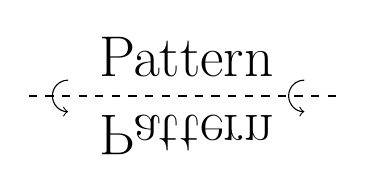
\begin{tikzpicture}
        % Draw the dashed line
        \draw[thick,dashed] (-2,0) -- (2,0);
        % Draw arcs
        \draw[->] (-1.5,0.2) arc (90:270:0.2);
        \draw[->] (1.5,0.2) arc (90:270:0.2);
        % Normal text above the line
        \node at (0,0.5) {\huge Pattern};
        % Mirrored text below the line
            \node[rotate=180] at (0,-0.5) {\reflectbox{\huge Pattern}};
    \end{tikzpicture}
    \caption{Reflections}
    \label{Reflection}
\end{subfigure}
\hfill
\begin{subfigure}{0.45\linewidth}
    \centering
    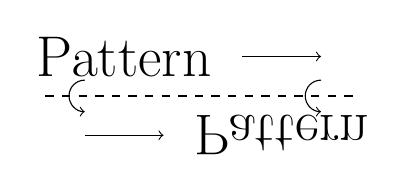
\begin{tikzpicture}
        % Draw the dashed line
        \draw[thick,dashed] (-2,0) -- (2,0);
        % Draw arcs
        \draw[->] (-1.5,0.2) arc (90:270:0.2);
        \draw[->] (1.5,0.2) arc (90:270:0.2);
        % Draw glide
        \draw[->] (0.5,0.5) -- (1.5,0.5);
        \draw[->] (-1.5,-0.5) -- (-0.5,-0.5);
        % Normal text above the line
        \node at (-1,0.5) {\huge Pattern};
        % Mirrored text below the line
            \node[rotate=180] at (1,-0.5) {\reflectbox{\huge Pattern}};
    \end{tikzpicture}
    \caption{Glide Reflection}
    \label{GlideReflection}
\end{subfigure}

\end{document}
        \caption{Reflective Symmetries}
        \label{fig:symmetries}
    \end{figure}
\end{frame}

\begin{frame}{Rotations}
    \begin{definition}
        A rotation is a change of angle around a center point.
        $R_\theta = \begin{bmatrix}
            \cos\theta & -\sin\theta\\
            \sin\theta & \cos\theta
        \end{bmatrix}$ 
        Where $\theta \in \{1,2,3,6\}.$ \cite{Angela:2023}
    \end{definition}
    \begin{figure}
        \centering
        \documentclass[class=article, crop=false]{standalone}
\usepackage{tikz}
\usepackage{subcaption}
\usetikzlibrary{calc}

\begin{document}

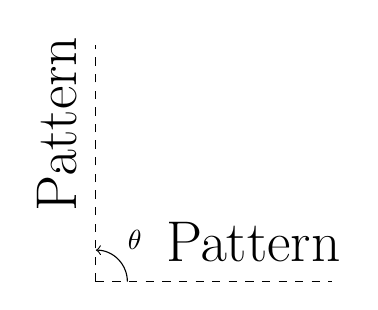
\begin{tikzpicture}
    \node[rotate=0] at ($(0:1) + (1,0.5)$) {\huge Pattern};
    \node[rotate=90] at ($(90:1) +(-0.5,1)$) {\huge Pattern};
    % Axis of rotation
    \draw[dashed] (0,0) -- (3,0);
    \draw[dashed] (0,0) -- (0,3);

    \draw[->] (0.4,0) arc (0:90:0.4) node[midway, above right] {$\theta$};
    %\node[] at (0,0) {o}
\end{tikzpicture}

\end{document}
        \caption{Rotations}
        \label{fig:enter-label}
    \end{figure}
\end{frame}

\begin{frame}{Lattices}
    \begin{definition}
        A lattice is the group $(\mathbb{Z}[\Vec{a},\Vec{b}],+).$\\
        i.e., a grid of points where any point $p = n\Vec{a} +m\Vec{b}$ 
    \end{definition}
    \begin{figure}
        \centering
        \scalebox{0.5}{\documentclass[class=article, crop=false]{standalone}
\usepackage{tikz}
\usepackage{subcaption}
\usetikzlibrary{calc}

\begin{document}
\begin{tikzpicture}
            \def\a{2}  % length of side a
            \def\b{3}  % length of side b

            \foreach \i in {0,...,6} {
                \foreach \j in {0,...,3} {
                     \fill[blue]  (\i*\a,\j*\b) circle(3.5pt);
                }
            }
            % Draw vector
            \coordinate (P) at (3*\a, 2*\b);
            \draw[thick,->] (0,0) -- (P) node[above right] {\huge $p$};

            % Draw lattice parameters
            \draw (0,0) -- (\a,0) node[midway,below] {\huge$\Vec{b}$};
            \draw (0,0) -- (0,\b) node[midway,left] {\huge$\Vec{a}$};
        \end{tikzpicture}
\end{document}}
        \caption{Lattice}
        \label{fig:enter-label}
    \end{figure}
\end{frame}

\begin{frame}{Bravais Lattices}
    \begin{minipage}{0.35\textwidth}
        Primitive cells are parallelograms, whereas centered cells have lattice points in the center.

        Additionally, Square $\subseteq$ Rectangle $\subseteq$ Rhombic,
        The Rectangle $\subseteq$ Oblique cell and the Hexagonal cell $\subseteq$ Oblique Cell.
    \end{minipage}
    \hfill
    \begin{minipage}{0.6\textwidth}
        \centering
        \scalebox{0.6}{\documentclass[class=article, crop=false]{standalone}
\usepackage{graphicx}
\usepackage{tikz}
\usepackage{subcaption}
\usetikzlibrary{calc}
\usepackage{import}

\begin{document}
\begin{minipage}{0.3\linewidth}
    \centering
    \begin{subfigure}{0.45\linewidth}
        \centering
        \documentclass[class=article, crop=false]{standalone}
\usepackage{tikz}
\usepackage{subcaption}
\usetikzlibrary{calc}

\begin{document}
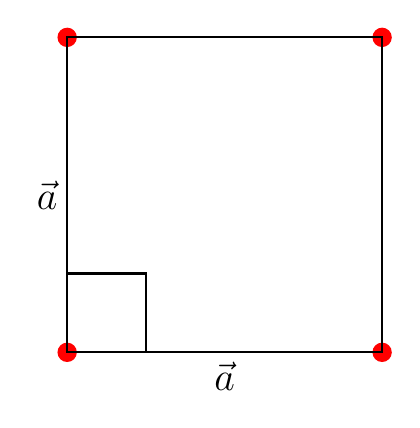
\begin{tikzpicture}
    \def\a{4}  % length of side a

    % Calculate the coordinates of the points
    \coordinate (A) at (0, 0);
    \coordinate (B) at (\a, 0);
    \coordinate (C) at (\a, \a);
    \coordinate (D) at (0, \a);

    \fill[red]  (A) circle(3.5pt) (B) circle(3.5pt) (C) circle(3.5pt) (D) circle(3.5pt);

    % Draw the square unit cell
    \draw[thick] (A) -- (B) -- (C) -- (D) -- cycle;

    % Draw right angle
    \draw[thick] (0,1) -- (1,1) -- (1,0);

    %Draw lattice parameters
    \node[left] at ($(A)!0.5!(D)$) {\Large $\vec{a}$};
    \node[below] at ($(A)!0.5!(B)$) {\Large $\vec{a}$};
    
\end{tikzpicture}
\end{document}
        \caption*{Square Cell}
        \label{fig:square-cell}
    \end{subfigure}
    \vfill
    \begin{subfigure}{0.45\textwidth}
        \centering
        \documentclass[class=article, crop=false]{standalone}
\usepackage{tikz}
\usepackage{subcaption}
\usetikzlibrary{calc}

\begin{document}
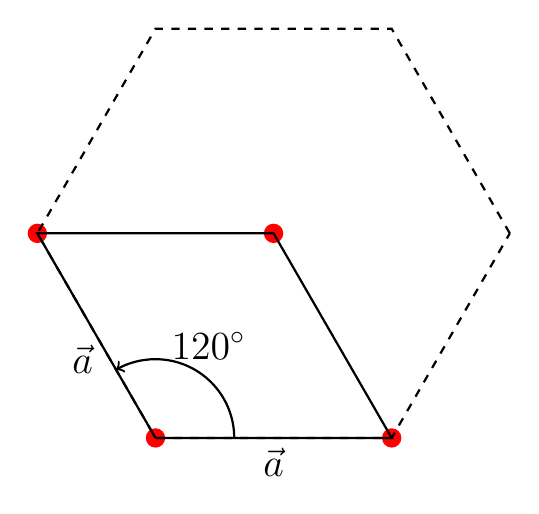
\begin{tikzpicture}
    \def\a{3}  % length of side a

    Calculate the coordinates of the points
    \coordinate (A) at (0:\a);
    \coordinate (B) at (60:\a);
    \coordinate (C) at (120:\a);
    \coordinate (D) at (180:\a);
    \coordinate (E) at (240:\a);
    \coordinate (F) at (300:\a);
    \coordinate (G) at (0,0);


    % Creates nodes at vertices
    \fill[red]  (D) circle(3.5pt) (E) circle(3.5pt) (F) circle(3.5pt) (G) circle(3.5pt);
    

    % Draw the hexagon boundary
    \draw[thick,dashed] (A) -- (B) -- (C) -- (D) -- (E) -- (F) -- (A);

    % Draw the cell
    \draw[thick] (E) -- (F) -- (G) -- (D) -- (E); 

    %Draw lattice parameters
    \node[anchor={60}] at ($(D)!0.5!(E)$) {\Large $\vec{a}$};
    \node[below] at ($(E)!0.5!(F)$) {\Large $\vec{a}$};

    % Optional: add angle markers
    \draw[thick, ->] (E) ++(1,0) arc[start angle=0, end angle=120, radius=1] node[midway,anchor={-120}] {\Large $120^\circ$};
    
\end{tikzpicture}
\end{document}
        \caption*{Hexagon Cell}
        \label{fig:hexagon-cell}
    \end{subfigure}
\end{minipage}
\hspace{2cm}
\begin{minipage}{0.9\linewidth}
    \centering
    \begin{subfigure}{0.45\linewidth}
        \centering
        \documentclass[class=article, crop=false]{standalone}
\usepackage{tikz}
\usepackage{subcaption}
\usetikzlibrary{calc}

\begin{document}

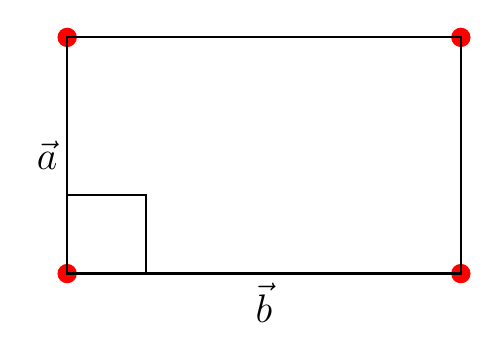
\begin{tikzpicture}
    \def\a{5}  % length of side a
    \def\b{3}  % length of side b
    \def\y{5}

    % Calculate the coordinates of the points
    \coordinate (A) at (0, 0);
    \coordinate (B) at (\a, 0);
    \coordinate (C) at (\a, \b);
    \coordinate (D) at (0, \b);

    %\coordinate (A2) at (0, 0 - \y);
    %\coordinate (B2) at (\a, 0- \y);
    %\coordinate (C2) at (\a, \b - \y);
    %\coordinate (D2) at (0, \b - \y);

    % Creates nodes at vertices
    \fill[red]  (A) circle(3.5pt) (B) circle(3.5pt) (C) circle(3.5pt) (D) circle(3.5pt);% (A2) circle(3.5pt) (B2) circle(3.5pt) (C2) circle(3.5pt) (D2) circle(3.5pt);
    %\fill[blue] ($(A2)!0.5!(C2)$) circle(3.5pt);

    % Draw right angle
    \draw[thick] (0,1) -- (1,1) -- (1,0);
    %\draw[thick] (0,1-\y) -- (1,1-\y) -- (1,0-\y);

    % Draw the rectangular unit cell
    \draw[thick] (A) -- (B) -- (C) -- (D) -- cycle;
    %\draw[thick] (A2) -- (B2) -- (C2) -- (D2) -- cycle;
    %\draw[dashed] (A2) -- (C2);
    %\draw[dashed] (B2) -- (D2);


    %Draw lattice parameters
    \node[left] at ($(A)!0.5!(D)$) {\Large $\vec{a}$};
    \node[below] at ($(A)!0.5!(B)$) {\Large $\vec{b}$};
    %\node[left] at ($(A2)!0.5!(D2)$) {\Large $\vec{a}$};
    %\node[below] at ($(A2)!0.5!(B2)$) {\Large $\vec{b}$};
    
\end{tikzpicture}
        
\end{document}
        \caption*{Rectangle Cell}
        \label{fig:rectangle-cell}
    \end{subfigure}  
    \vfill
    \begin{subfigure}{0.45\linewidth}
        \centering
        \documentclass[class=article, crop=false]{standalone}
\usepackage{tikz}
\usepackage{subcaption}
\usetikzlibrary{calc}

\begin{document}
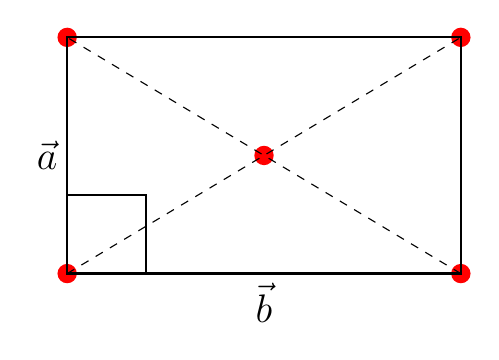
\begin{tikzpicture}
    \def\a{5}  % length of side a
    \def\b{3}  % length of side b

    % Calculate the coordinates of the points
    \coordinate (A) at (0, 0);
    \coordinate (B) at (\a, 0);
    \coordinate (C) at (\a, \b);
    \coordinate (D) at (0, \b);
    %\coordinate (E) at (\a, 2*\b);
    %\coordinate (F) at (0, 2*\b);

    % Creates node labels
    %\node[above left] at (A) {A};
    %\node[above left] at (B) {B};
    %\node[above left] at (C) {C};
    %\node[above left] at (D) {D};
    %\node[above left] at (E) {E};
    %\node[above left] at (F) {F};

    % Creates nodes at vertices
    \fill[red]  (A) circle(3.5pt) (B) circle(3.5pt) (C) circle(3.5pt) (D) circle(3.5pt);% (E) circle(3.5pt) (F) circle(3.5pt);
    % Creates nodes at centers
    \fill[red] ($(A)!0.5!(C)$) circle(3.5pt);
    %\fill[blue] ($(D)!0.5!(E)$) circle(3.5pt);

    % Draw the rectangular unit cell
    \draw[thick] (A) -- (B) -- (C) -- (D) -- cycle;
    %\draw[thick,dashed] (D) -- (F) -- (E) -- (C) -- cycle;
    %\draw[thick] (D) -- ($(A)!0.5!(C)$) -- (C) -- ($(D)!0.5!(E)$) -- cycle;

    % Draw lines
    \draw[dashed] (A) -- (C);
    \draw[dashed] (B) -- (D);

    % Draw right angle
    \draw[thick] (0,1) -- (1,1) -- (1,0);


    %Draw lattice parameters
    \node[left] at ($(A)!0.5!(D)$) {\Large $\vec{a}$};
    \node[below] at ($(A)!0.5!(B)$) {\Large $\vec{b}$};
    
\end{tikzpicture}

\end{document}
        \caption*{Rhombic Cell}
        \label{fig:rhombic-cell}
    \end{subfigure}
    \vfill
    % Oblique
    \begin{subfigure}{0.45\linewidth}
        \centering
        \documentclass[class=article, crop=false]{standalone}
\usepackage{tikz}
\usepackage{subcaption}
\usetikzlibrary{calc}

\begin{document}
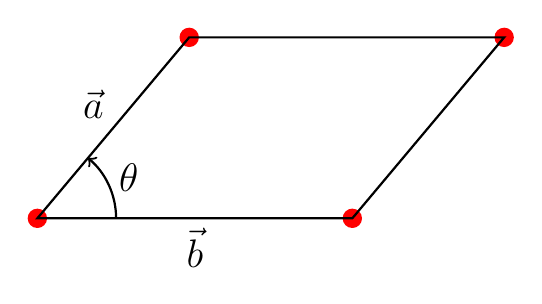
\begin{tikzpicture}
    % Define the lengths of the sides and the angle
    \def\a{4}  % length of side a
    \def\b{3}  % length of side b
    \def\angle{50}  % angle between sides a and b

    % Calculate the coordinates of the points
    \coordinate (A) at (0, 0);
    \coordinate (B) at (\a, 0);
    \coordinate (C) at ({\a + \b*cos(\angle)}, {\b * sin(\angle)});
    \coordinate (D) at ({\b * cos(\angle)}, {\b * sin(\angle)});

    
    % Creates nodes at vertices
    \fill[red]  (A) circle(3.5pt) (B) circle(3.5pt) (C) circle(3.5pt) (D) circle(3.5pt);

    % Draw the oblique unit cell
    \draw[thick] (A) -- (B) -- (C) -- (D) -- cycle;

    %Draw lattice parameters
    \node[anchor={-\angle}] at ($(A)!0.5!(D)$) {\Large $\vec{a}$};
    \node[below] at ($(A)!0.5!(B)$) {\Large $\vec{b}$};
    
    % Optional: add angle markers
    \draw[thick, ->] (A) ++(1,0) arc[start angle=0, end angle=\angle, radius=1] node[midway, anchor={150+\angle}] {\Large $\theta$};
\end{tikzpicture}
\end{document}
        \caption*{Oblique Cell}
        \label{fig:oblique-cell}
    \end{subfigure}
\end{minipage}

\end{document}}
        \captionof{figure}{Bravais Lattices}
        \label{fig:lattice}
    \end{minipage}
\end{frame}
\begin{frame}{Visual proof that lattices cannot have order 8}
\begin{figure}
    \centering
    \begin{minipage}{0.3\textwidth}
        \scalebox{0.5}{\documentclass[class=article, crop=false]{standalone}
\usepackage{tikz}
\usepackage{subcaption}
\usetikzlibrary{calc}
\usepackage{amsmath}

\begin{document}
\begin{tikzpicture}
    % Define the number of sides and the radius
    \def\sides{8}
    \def\radius{3}
    \def\smallradius{2.3}
    \def\angle{360/\sides}
    \def\sidelength{2*\radius*sin(180/\sides)} % Side length of the first octagon

    %\def\smallradius{{\sin(\angle)}}

    
    \fill[red]  (0,0) circle(3.5pt);
    
    \fill  \foreach \i in {0,...,\sides} {(\i*\angle:\radius) circle(3.5pt)};

    %\fill[red]  \foreach \i in {0,...,\sides} {(\i*\angle-0.5*\angle:\smallradius) circle(3.5pt)};
    
    % Draw the first octagon using a foreach loop
    %\draw[thick]
        \foreach \i in {0,1,...,\sides} {
            (\i*\angle:\radius) -- (\i*\angle+\angle:\radius)
        } -- cycle;


    % Draw the second octagon shifted by half a side length
    %\draw[thick, red]
        \foreach \i in {0,1,...,\sides} {
            (\i*\angle-0.5*\angle:\sidelength) -- (\i*\angle+0.5*\angle:\sidelength)
    } -- cycle;


    \draw[blue] (1*\angle:\radius) -- (2*\angle:\radius){};
    \draw[blue] (0,0) --($(5*\angle:\radius) - (6*\angle:\radius)$){};
    
\end{tikzpicture}
\end{document}}
        \caption{1}
    \end{minipage}
    \hfill
    \begin{minipage}{0.3\textwidth}
        \scalebox{0.5}{\documentclass[class=article, crop=false]{standalone}
\usepackage{tikz}
\usepackage{subcaption}
\usetikzlibrary{calc}
\usepackage{amsmath}

\begin{document}
\begin{tikzpicture}
    % Define the number of sides and the radius
    \def\sides{8}
    \def\radius{3}
    \def\smallradius{2.3}
    \def\sm{1.24}
    \def\angle{360/\sides}
    \def\sidelength{2*\radius*sin(180/\sides)} % Side length of the first octagon
    \def\sidelength2{\radius*sin(180/\sides)} % Side length of the first octagon

    %\def\smallradius{{\sin(\angle)}}

    
    \fill[red]  (0,0) circle(3.5pt);
    
    \fill  \foreach \i in {0,...,\sides} {(\i*\angle:\radius) circle(3.5pt)};

    \fill[red]  \foreach \i in {0,...,\sides} {(\i*\angle-0.5*\angle:\smallradius) circle(3.5pt)};

    \fill[blue]  \foreach \i in {0,...,\sides} {(\i*\angle:\sm) circle(3.5pt)};
    
    % Draw the first octagon using a foreach loop
    %\draw[thick]
        \foreach \i in {0,1,...,\sides} {
            (\i*\angle:\radius) -- (\i*\angle+\angle:\radius)
        } -- cycle;


    % Draw the second octagon shifted by half a side length
    %\draw[thick, red]
        \foreach \i in {0,1,...,\sides} {
            (\i*\angle-0.5*\angle:\sidelength) -- (\i*\angle+0.5*\angle:\sidelength)
    } -- cycle;


    %\draw[blue] ($(5*\angle:\radius) - (6*\angle:\radius)$) -- (5*\angle:\radius){};
    \draw[blue] ($(0,0) - (4*\angle:\radius)$) --($(5*\angle:\radius) - (6*\angle:\radius) - (4*\angle:\radius)$){};
    \draw[blue] (0,0) --($(5*\angle:\radius) - (6*\angle:\radius)$){};
    \draw[blue] (1*\angle:\radius) -- (2*\angle:\radius){};
    
\end{tikzpicture}
\end{document}}
        \caption{2}
    \end{minipage}
    \hfill
    \begin{minipage}{0.3\textwidth}
        \scalebox{0.5}{\documentclass[class=article, crop=false]{standalone}
\usepackage{tikz}
\usepackage{subcaption}
\usetikzlibrary{calc}
\usepackage{amsmath}

\begin{document}
\begin{tikzpicture}
    % Define the number of sides and the radius
    \def\sides{8}
    \def\radius{3}
    \def\smallradius{2.3}
    \def\sm{1.24}
    \def\smm{0.94}
    \def\smmm{0.51}
    \def\angle{360/\sides}
    \def\sidelength{2*\radius*sin(180/\sides)} % Side length of the first octagon
    \def\sidelength2{\radius*sin(180/\sides)} % Side length of the first octagon

    %\def\smallradius{{\sin(\angle)}}

    
    \fill[red]  (0,0) circle(3.5pt);
    
    \fill  \foreach \i in {0,...,\sides} {(\i*\angle:\radius) circle(3.5pt)};

    \fill[red]  \foreach \i in {0,...,\sides} {(\i*\angle-0.5*\angle:\smallradius) circle(3.5pt)};

    \fill[blue]  \foreach \i in {0,...,\sides} {(\i*\angle:\sm) circle(3.5pt)};

    \fill[green]  \foreach \i in {0,...,\sides} {(\i*\angle-0.5*\angle:\smm) circle(3.5pt)};

    \fill[pink]  \foreach \i in {0,...,\sides} {(\i*\angle:\smmm) circle(3.5pt)};

    
    % Draw the first octagon using a foreach loop
    %\draw[thick]
        \foreach \i in {0,1,...,\sides} {
            (\i*\angle:\radius) -- (\i*\angle+\angle:\radius)
        } -- cycle;


    % Draw the second octagon shifted by half a side length
    %\draw[thick, red]
        \foreach \i in {0,1,...,\sides} {
            (\i*\angle-0.5*\angle:\sidelength) -- (\i*\angle+0.5*\angle:\sidelength)
    } -- cycle;


    %\draw[blue] ($(5*\angle:\radius) - (6*\angle:\radius)$) -- (5*\angle:\radius){};
    \draw[blue] ($(0,0) - (4*\angle:\sm)$) --($(5*\angle:\sm) - (6*\angle:\sm) - (4*\angle:\sm)$){};
    \draw[blue] (0,0) --($(5*\angle:\sm) - (6*\angle:\sm)$){};
    \draw[blue] (1*\angle:\sm) -- (2*\angle:\sm){};
    
\end{tikzpicture}
\end{document}}
        \caption{3}
    \end{minipage}
    \caption{Octagons under translation}
    \label{fig:enter-label}
\end{figure}
    \begin{block}{Proof sketch}
        Note that any point can translated by lattice definition. So the translation of the center and vertices gives two smaller octagons. This can further be extended in smaller octagons. This can be repeated infinitely. Creating a dense grid of points on the entire 2-dimensional plane.
    \end{block}
\end{frame}

\begin{frame}{Frieze Groups}
    \begin{definition}
        A frieze group is the set of two-dimensional patterns that repeat in one dimension. \cite{Ganapathy:2021}
    \end{definition}
    \begin{figure}
        \centering
        \documentclass[class=article, crop=false]{standalone}
\usepackage{tikz}
\usepackage{subcaption}
\usetikzlibrary{calc}

\begin{document}

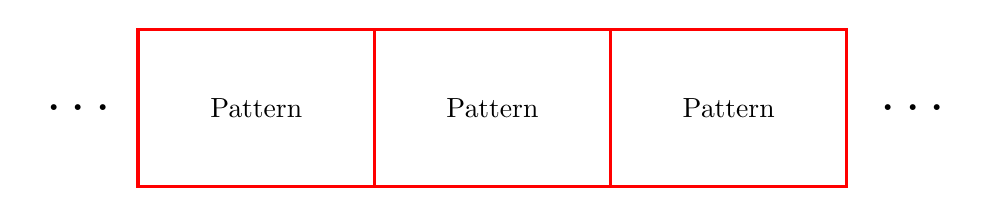
\begin{tikzpicture}
    \node[scale=2] at (-0.2, 1) {\ldots};
    \foreach \j in {0,...,2} {
        \draw[red, very thick] (0.5+3*\j,0) rectangle (3.5+3*\j,2);
        \node at (2 + 3*\j, 1) {Pattern};
    }
    % Add ellipsis at the end
    \node[scale=2] at (10.4, 1) {\ldots};
\end{tikzpicture}

\end{document}
        \caption{Frieze group example}
        \label{fig:enter-label}
    \end{figure}
\end{frame}

\begin{frame}{Frieze Groups}
    \begin{figure}
    \centering
	\documentclass[class=article, crop=false]{standalone}
\usepackage{tikz}
\usepackage{subcaption}
\usetikzlibrary{calc}

\begin{document}

\begin{subfigure}{0.21\linewidth}
        \centering
		
\includegraphics[width=\linewidth, angle=90]{Figures/Frieze groups/Frieze_hop.png}
		\caption{p1}
		\label{fig:p1}
	\end{subfigure}
	\begin{subfigure}{0.21\linewidth}
        \centering
		
\includegraphics[width=\linewidth,angle=90]{Figures/Frieze groups/Frieze_jump.png}
		\caption{p11m}
		\label{fig:p11m}
	\end{subfigure}
	\begin{subfigure}{0.21\linewidth}
            \centering
	        
\includegraphics[width=\linewidth,angle=90]{Figures/Frieze groups/Frieze_sidle.png}
	        \caption{p1m1}
	        \label{fig:p1m1}
    \end{subfigure}
    \begin{subfigure}{0.21\linewidth}
            \centering
	        
\includegraphics[width=\linewidth,angle=90]{Figures/Frieze groups/Frieze_step.png}
	        \caption{p11g}
	        \label{fig:p11g}
    \end{subfigure}
    \vfill
    \begin{subfigure}{0.21\linewidth}
            \centering
	        
\includegraphics[width=\linewidth,angle=90]{Figures/Frieze groups/Frieze_spinning_hop.png}
	        \caption{p2}
	        \label{fig:p2}
    \end{subfigure}
    \begin{subfigure}{0.21\linewidth}
            \centering
	        
\includegraphics[width=\linewidth,angle=90]{Figures/Frieze groups/Frieze_spinning_jump.png}
	        \caption{p2mm}
	        \label{fig:p2mm}
    \end{subfigure}
    \begin{subfigure}{0.21\linewidth}
            \centering
	        
\includegraphics[width=\linewidth,angle=90]{Figures/Frieze groups/Frieze_spinning_sidle.png}
	        \caption{p2mg}
	        \label{fig:subfigC}
    \end{subfigure}

    \end{document}
	\caption{The seven frieze groups \cite{Tomruen:2015}.}
	\label{fig:FriezeGroups}
\end{figure}
\end{frame}

\begin{frame}{Wallpaper Groups}
    \begin{definition}
        A wallpaper group is the set of isometries and a fundamental region that fill an entire two-dimensional Euclidean plane. \cite{Ganapathy:2021}
    \end{definition}
    \begin{figure}
        \centering
        \documentclass[class=article, crop=false]{standalone}
\usepackage{tikz}
\usepackage{subcaption}
\usetikzlibrary{calc}

\begin{document}

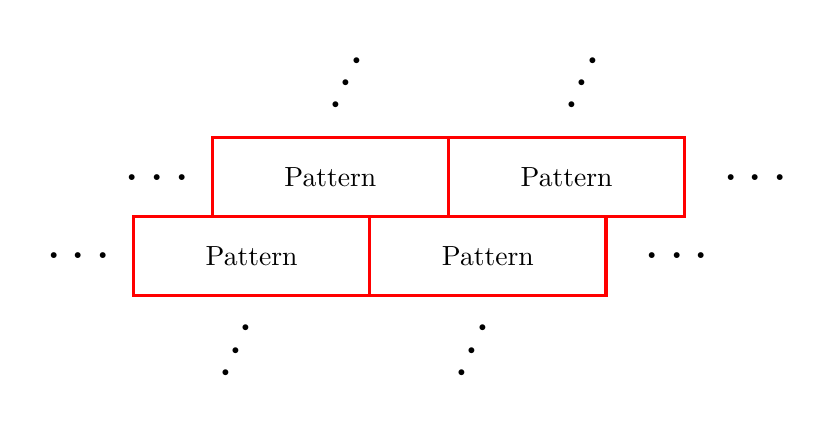
\begin{tikzpicture}
        % Add ellipses at start
        \node[scale=2] at (-0.2, .5) {$\ldots$};
        \node[scale=2] at (0.8, 1.5) {$\ldots$};
        \foreach \i in {0,...,1} {
            \foreach \j in {0,...,1} {
                \draw[red, very thick] (0.5+3*\i+\j,1*\j) rectangle (3.5+3*\i+\j,1*\j+1);
                \node at (2 + 3*\i+\j, 1*\j+.5) {Pattern};
        }}
        % Add ellipses at the end
        \node[scale=2] at (7.4, .5) {$\ldots$};
        \node[scale=2] at (8.4, 1.5) {$\ldots$};
        % Add ellipses above
        \node[scale=2,rotate=-115] at (3.2, 2.7) {$\ldots$};
        \node[scale=2,rotate=-115] at (6.2, 2.7) {$\ldots$};
        % Add ellipses below
        \node[scale=2,rotate=-115] at (1.8, -0.7) {$\ldots$};
        \node[scale=2,rotate=-115] at (4.8, -0.7) {$\ldots$};
    \end{tikzpicture}

\end{document}
        \caption{Wallpaper group example}
        \label{fig:enter-label}
    \end{figure}
\end{frame}

\begin{frame}{Symmetry group properties, IUC}
    \begin{table}
    \begin{tabular}{|c|c|c|c|}
        \hline
        Wallpaper Group & Lattice & Rotation order & Reflections \\
        \hline
        p1 & Oblique & 0 & none\\
        p2 & Oblique & 2 & none\\
        pm & Rectangle & 0 & 180$^\circ$\\
        pg & Rectangle & 0 & none\\
        cm & Rhombus & 0 & 180$^\circ$\\
        pmm & Rectangle & 2 & 90$^\circ$\\
        pmg & Rectangle & 2 & 180$^\circ$\\
        pgg & Rectangle & 2 & none\\
        cmm & Rhombus & 2 & 90$^\circ$\\
        \hline
    \end{tabular}   
    \caption{Symmetries of the wallpaper groups. \cite{Clark1}}
\end{table}
\end{frame}
\begin{frame}{Symmetry group properties, IUC}
    \begin{table}
        \begin{tabular}{|c|c|c|c|}
            \hline
            Wallpaper Group & Lattice & Rotation order & Reflections \\
            \hline
            p4 & Square & 4 & none\\
            p4m & Square & 4$^\dagger$ & 45$^\circ$\\
            p4g & Square & 4$^*$ & 90$^\circ$\\
            p3 & Hexagon & 3 & none\\
            p31m & Hexagon & 3$^*$ & 60$^\circ$\\
            p3m1 & Hexagon & 3$^\dagger$ & 30$^\circ$\\
            p6 & Hexagon & 6 & none\\
            p6m & Hexagon & 6 & 30$^\circ$\\
            \hline
        \end{tabular}
    \caption{Symmetries of the wallpaper groups: $\dagger$ means the rotation centres lie on the reflection axis. * means the group rotation centres are not on the reflection axis. \cite{Clark1}}
\end{table}
\end{frame}

\begin{frame}
\frametitle{Wall Paper Groups}
    \begin{block}{Why are they A group}
        They meet the three group axioms
        \begin{itemize}
            \item Identity: no transformations.
            \item Inverses: the reversal or opposite of the transformation.
            \item Associativity: two transformations are still a transformation. \cite{Angela:2023}
        \end{itemize}       
    \end{block}
\end{frame}

\begin{frame}
  \frametitle{Wallpaper groups}
  \begin{columns}
          \column{0.5\linewidth}
  \begin{definition}
      \begin{itemize}
          \item P1 (primitive of order 1)\cite{Trefor1}
          \item simplest of the 17 groups 
          \item consists only of translations
      \end{itemize}
  \end{definition}/
  \column{0.4\textwidth}
  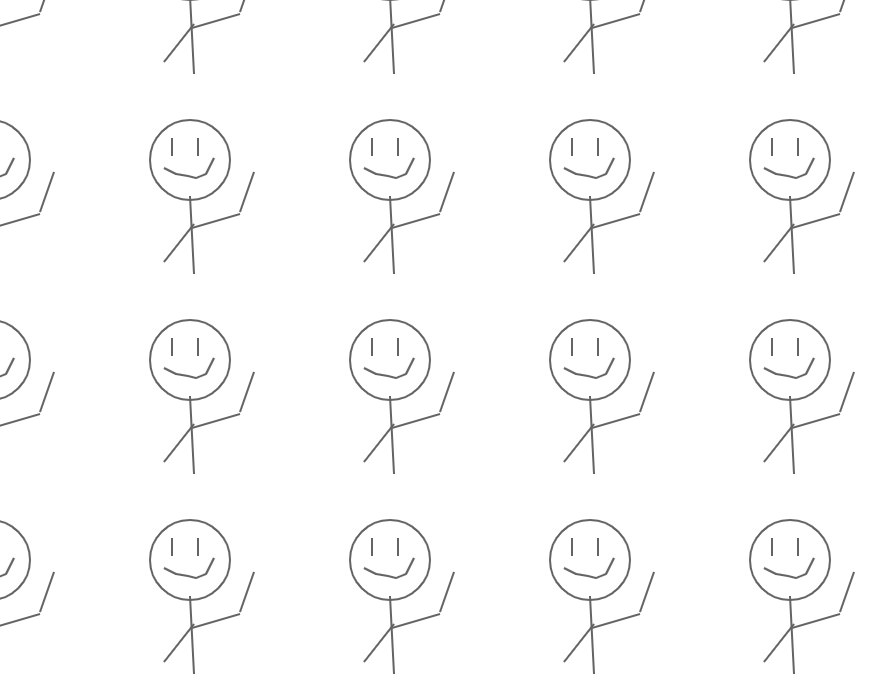
\includegraphics[width=\textwidth]{Figures/p_examples/eschersketch_p1_example_person.png}
  \end{columns}
  \begin{figure}
        \centering
        \scalebox{0.7}{\documentclass[class=article, crop=false]{standalone}
\usepackage{tikz}
\usepackage{subcaption}
\usetikzlibrary{calc}

\begin{document}
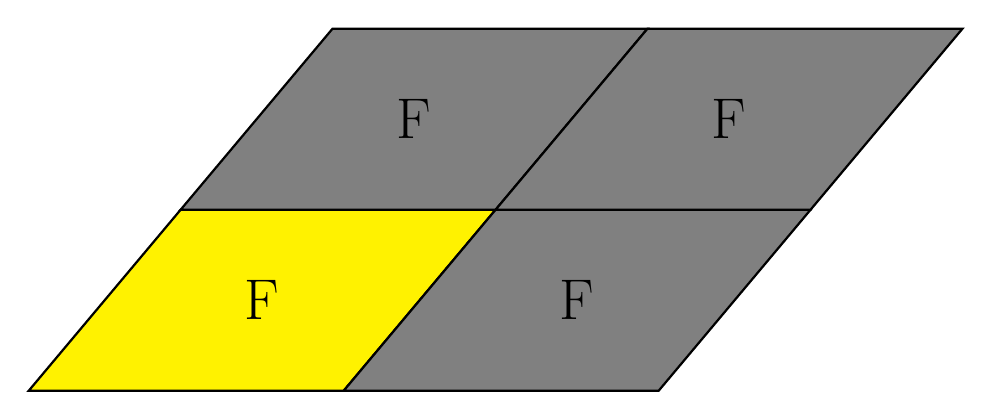
\begin{tikzpicture}
    % Define the lengths of the sides and the angle
    \def\a{4}  % length of side a
    \def\b{3}  % length of side b
    \def\angle{50}  % angle between sides a and b
    \def\s{F} % Label in center of cells

    % Calculate the coordinates of the points
    \coordinate (C00) at (0, 0);
    \coordinate (C10) at (\a, 0);
    \coordinate (C11) at ({\a + \b*cos(\angle)}, {\b * sin(\angle)});
    \coordinate (C01) at ({\b * cos(\angle)}, {\b * sin(\angle)});
    \coordinate (C02) at ({2*\b*cos(\angle)}, {2*\b * sin(\angle)});
    \coordinate (C12) at ({\a +2*\b * cos(\angle)}, {2*\b * sin(\angle)});
    \coordinate (C22) at ({2*\a + 2*\b * cos(\angle)}, {2*\b * sin(\angle)});
    \coordinate (C21) at ({2*\a + \b*cos(\angle)}, {\b * sin(\angle)});
    \coordinate (C20) at ({2*\a}, 0);

        
    % Draw the oblique unit cell
    \draw[thick,fill=yellow] (C00) -- (C10) -- (C11) -- (C01) -- cycle;
    \draw[thick,fill=gray] (C01) -- (C11) -- (C12) -- (C02) -- cycle;
    \draw[thick,fill=gray] (C10) -- (C20) -- (C21) -- (C11) -- cycle;
    \draw[thick,fill=gray] (C11) -- (C21) -- (C22) -- (C12) -- cycle;

    % Center symbols
    \node at ($(C00)!0.5!(C11)$) {\huge \s};
    \node at ($(C20)!0.5!(C11)$) {\huge \s};
    \node at ($(C02)!0.5!(C11)$) {\huge \s};
    \node at ($(C22)!0.5!(C11)$) {\huge \s};
\end{tikzpicture}
\end{document}}
        \caption{p1 diagram}
        \label{fig:p1}
  \end{figure}
\end{frame}

\begin{frame}
\frametitle{more examples of wallpaper groups}
    \begin{figure}
     \centering
     \begin{subfigure}[b]{0.3\textwidth}
         \centering
         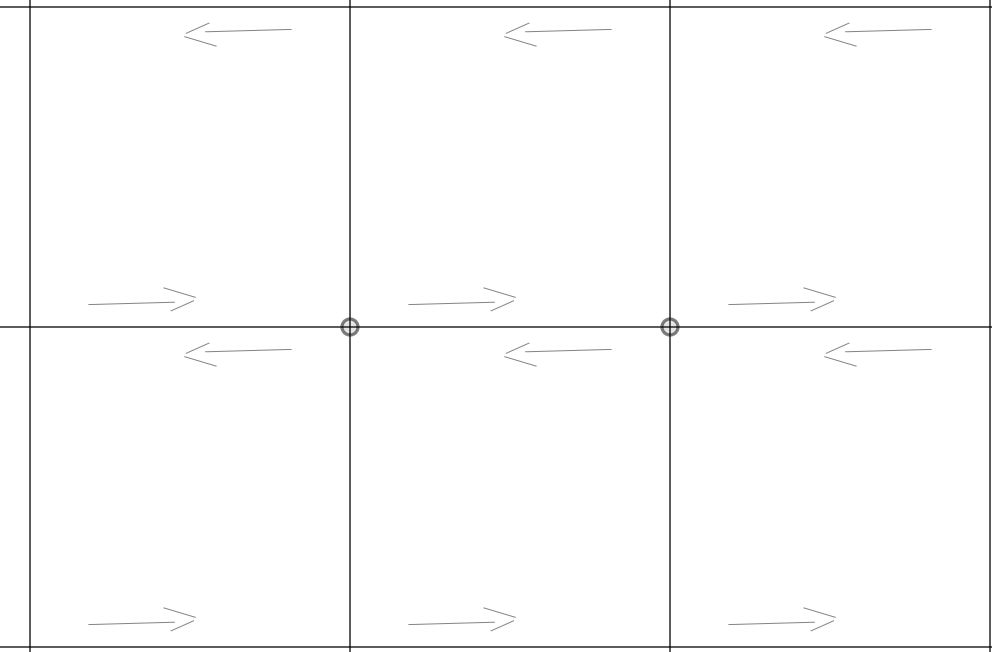
\includegraphics[width=\textwidth]{Figures/p_examples/p_2_simple.JPG}
         \caption{p2}
         \label{fig: p2}
     \end{subfigure}
     \hfill
     \begin{subfigure}[b]{0.3\textwidth}
         \centering
         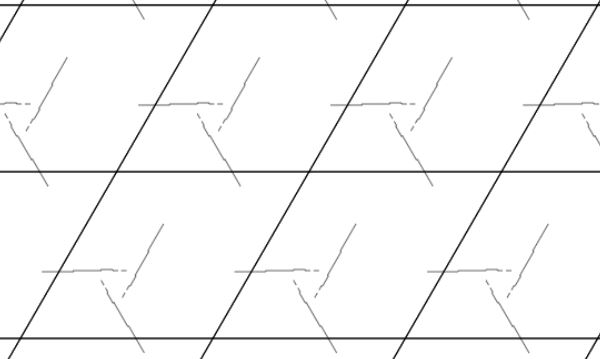
\includegraphics[width=\textwidth]{Figures/p_examples/p_3_simple.JPG}
         \caption{p3}
         \label{fig:p3}
     \end{subfigure}
     \vfill
     \begin{subfigure}[b]{0.3\textwidth}
         \centering
         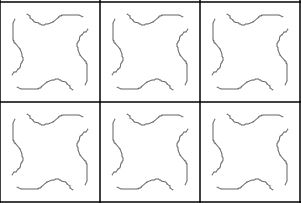
\includegraphics[width=\textwidth]{Figures/p_examples/p_4_simple_two.JPG}
         \caption{p4}
         \label{fig:p4}
     \end{subfigure}
     \hfill
     \begin{subfigure}[b]{0.3\textwidth}
         \centering
         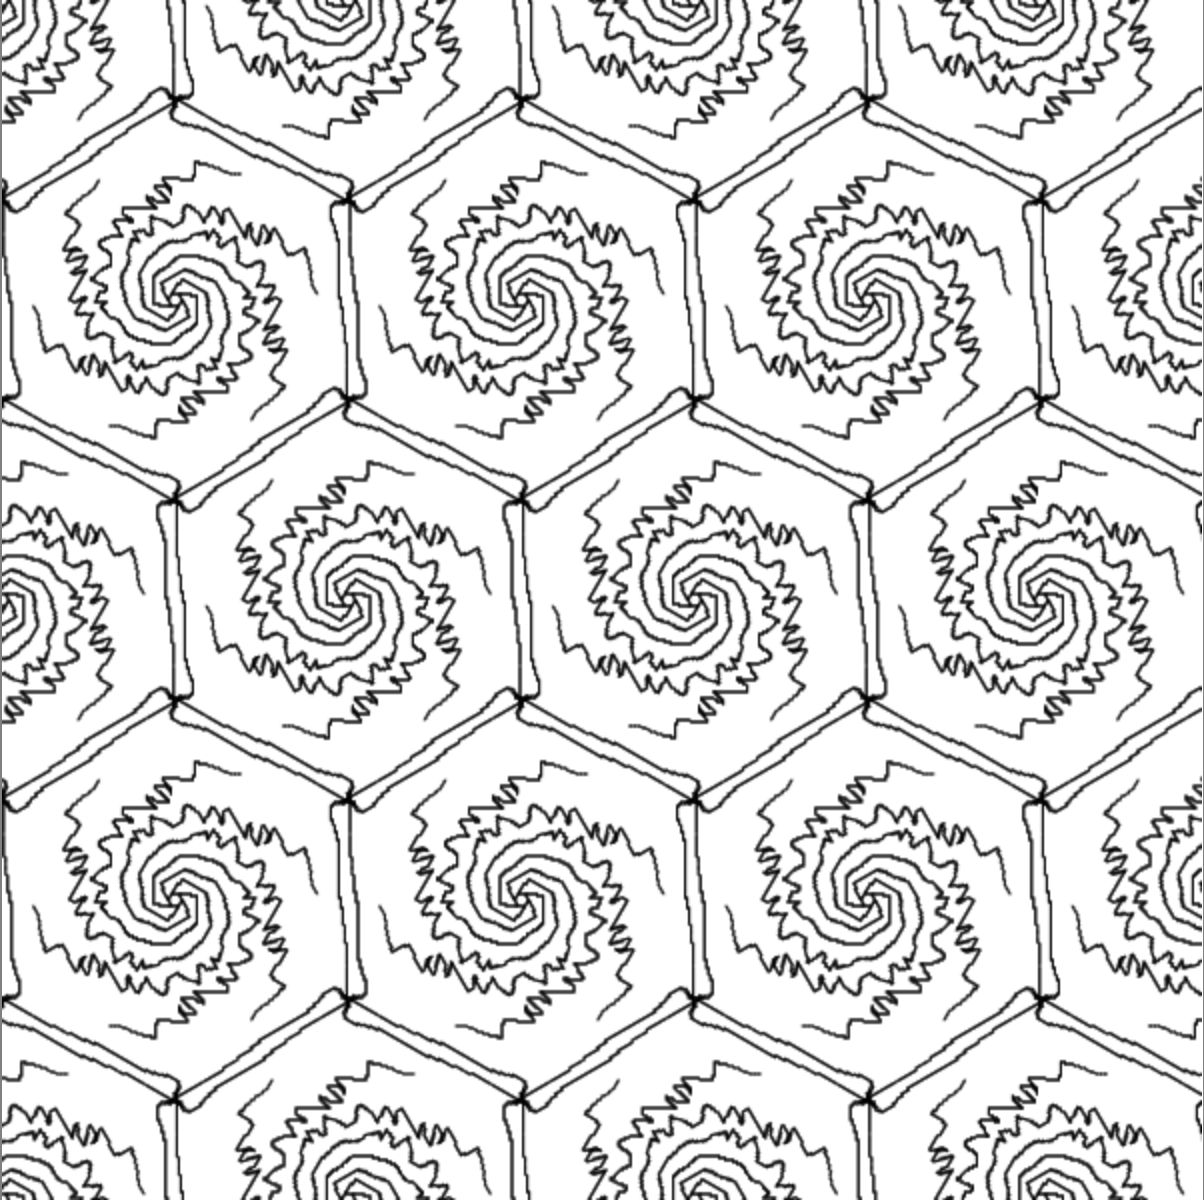
\includegraphics[width=\textwidth]{Figures/p_examples/P6.png}
         \caption{p6}
         \label{fig:p6}
     \end{subfigure}
        \caption{Four of the simplest wallpaper groups}
        \label{fig:The four ps}       
\end{figure}
\end{frame}
    
\begin{frame}{p6m}
    \begin{figure}{\textwidth}
        \centering
        \begin{minipage}{0.6\textwidth}
            \centering
            \begin{subfigure}[b]{\textwidth}
                \centering
                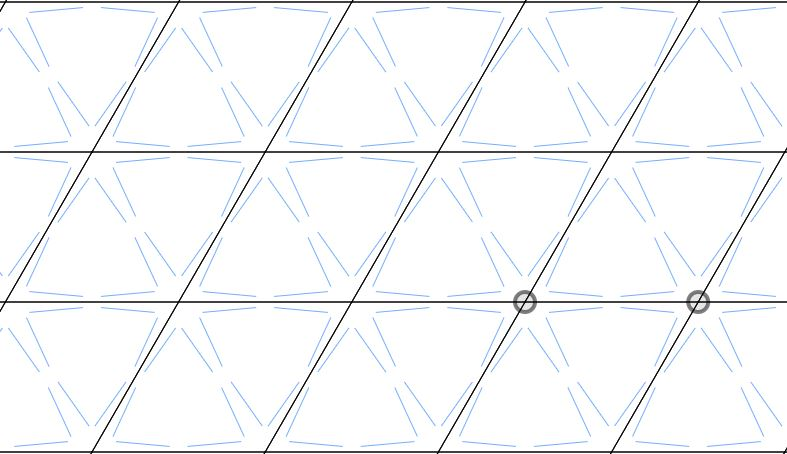
\includegraphics[width=0.5\textwidth]{Figures/p6m/p6m_full.JPG}
                \caption{Image of p6m}
                \label{fig:p6m_full}
            \end{subfigure}
            \vfill
            \begin{subfigure}[b]{\linewidth}
                \centering
                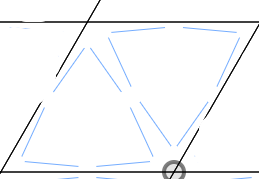
\includegraphics[width=0.5\linewidth]{Figures/p6m/p6m_simplified.png}
                \caption{p6m zoomed into one cell}
                \label{fig:p6m_zoomed}
            \end{subfigure}
        \end{minipage}
        \hspace{-2cm} % Adjust this value to control the space
        \begin{minipage}{0.35\textwidth}
            \begin{subfigure}[b]{\textwidth}
                \centering
                \scalebox{0.55}{\documentclass[class=article, crop=false]{standalone}
\usepackage{tikz}
\usepackage{subcaption}
\usetikzlibrary{calc}
\usetikzlibrary {shapes.geometric}

\begin{document}
\begin{tikzpicture}
    % Define the lengths of the sides and the angle
    \def\a{3}  % length of side a
    \def\b{3}  % length of side b
    \def\angle{60}  % angle between sides a and b
    \def\s{T} % Label in center of cells

    % Calculate the coordinates of the points
    \coordinate (C00) at (0, 0);
g10) at (\a, 0);
    \coordinate (C11) at ({\a + \b*cos(\angle)}, {\b * sin(\angle)});
    \coordinate (C01) at ({\b * cos(\angle)}, {\b * sin(\angle)});
    \coordinate (C02) at ({2*\b*cos(\angle)}, {2*\b * sin(\angle)});
    \coordinate (C12) at ({\a +2*\b * cos(\angle)}, {2*\b * sin(\angle)});
    \coordinate (C22) at ({2*\a + 2*\b * cos(\angle)}, {2*\b * sin(\angle)});
    \coordinate (C21) at ({2*\a + \b*cos(\angle)}, {\b * sin(\angle)});
    \coordinate (C20) at ({2*\a}, 0);

    \coordinate (A1) at ($(C00)!0.6666!(C11)$);
    \coordinate (A2) at ($(C11)!0.3333!(C22)$);

    % Draw the oblique unit cell
    \draw[fill=gray] (C00) -- (C20) -- (C22) -- (C02) -- cycle;
    \draw[thick,fill=yellow] (C00) -- (C10) -- ($(C00)!0.6666!(C11)$) -- cycle;
    \draw[ultra thick,pink] (C00) -- (C20) -- (C22) -- (C02) -- cycle;
    \draw[ultra thick,pink] (C20) -- (C02);
    \draw[ultra thick,blue] (C00) -- (C22);
    \draw[ultra thick,blue] (C01) -- (C20);
    \draw[ultra thick,blue] (C10) -- (C02);
    \draw[ultra thick,blue] (C02) -- (C21);
    \draw[ultra thick,blue] (C20) -- (C12);
    
    % Draw mirrow lines
    \draw[dashed,blue] ($(C01)!0.5!(C02)$) -- ($(C20)!0.5!(C21)$);
    \draw[dashed,blue] ($(C10)!0.5!(C20)$) -- ($(C02)!0.5!(C12)$);
    \draw[dashed] (C01) -- (C21);
    \draw[dashed] (C10) -- (C12);
    \draw[dashed,red] (C01) -- (C12);
    \draw[dashed,red] (C10) -- (C21);
    \draw[dashed,red] (C01) -- (C10);
    \draw[dashed,red] (C21) -- (C12);
    \draw[dashed,red] (C01) -- ($(C00)!0.5!(C10)$);
    \draw[dashed,red] (C10) -- ($(C00)!0.5!(C01)$);
    \draw[dashed,red] (C21) -- ($(C12)!0.5!(C22)$);
    \draw[dashed,red] (C12) -- ($(C21)!0.5!(C22)$);
    
    % Draw chiral center
    \node at ($(C00)!0.5!(C10)!0.3333!(A1)$) {\huge \s};
    \node[rotate=240] at ($(C00)!0.5!(A1)!0.3333!(C01)$) {\reflectbox{\huge\s}};
    \node[rotate=0] at ($(C10)!0.5!(A1)!0.3333!(C20)$) {\reflectbox{\huge \s}};
    \node[rotate=120] at ($(A1)!0.5!(C11)!0.3333!(C20)$) {\huge \s};
    \node[rotate=300] at ($(C11)!0.5!(A2)!0.3333!(C20)$) {\reflectbox{\huge \s}};
    \node[rotate=60] at ($(C21)!0.5!(A2)!0.3333!(C20)$) {\huge \s};
    \node[rotate=60] at ($(C21)!0.5!(A2)!0.3333!(C22)$) {\reflectbox{\huge \s}};
    \node[rotate=180] at ($(C12)!0.5!(A2)!0.3333!(C22)$) {\huge \s};
    \node[rotate=300] at ($(C11)!0.5!(A2)!0.3333!(C02)$) {\huge \s};
    \node[rotate=180] at ($(C12)!0.5!(A2)!0.3333!(C02)$) {\reflectbox{\huge \s}};
    \node[rotate=240] at ($(C01)!0.5!(A1)!0.3333!(C02)$) {\huge \s};
    \node[rotate=120] at ($(C11)!0.5!(A1)!0.3333!(C02)$) {\reflectbox{\huge \s}};

    % Draw node reflections
    \draw (C00)  node[regular polygon, regular polygon sides=6, draw, fill=blue, minimum size=0.5cm] {};
    \draw (C10)  node[shape aspect=0.5, diamond,draw,fill=pink] {};
    \draw (C11)  node[shape aspect=0.5,diamond,draw,fill=pink] {};
    \draw (C01)  node[shape aspect=0.5,diamond,draw,fill=pink] {};
    \draw (C02)  node[regular polygon, regular polygon sides=6, draw, fill=blue, minimum size=0.5cm] {};
    \draw (C12)  node[shape aspect=0.5,diamond,draw,fill=pink] {};
    \draw (C22)  node[regular polygon, regular polygon sides=6, draw, fill=blue, minimum size=0.5cm] {};
    \draw (C21)  node[shape aspect=0.5,diamond,draw,fill=pink] {};
    \draw (C20)  node[regular polygon, regular polygon sides=6, draw, fill=blue, minimum size=0.5cm] {};

    \draw (A1)  node[regular polygon, regular polygon sides=3, draw, fill=red, minimum size=0.5cm] {};
    \draw (A2)  node[regular polygon, regular polygon sides=3, draw, fill=red, minimum size=0.5cm] {};
\end{tikzpicture}
\end{document}}
                \caption{p6m Diagram}
                \label{fig:p6m_diagram}
            \end{subfigure}
        \end{minipage}
        \caption{One of the most complex wallpaper groups}
        \label{fig:The four ps}
    \end{figure}
\end{frame}

\begin{frame}
  \frametitle{Conclusion}
  \begin{itemize}
    \item The 17 Wallpaper groups are a mathematical repetitive 2D pattern.
    \item There are 4 symmetries within each group: translation, rotation, reflection and glide reflection.
    \item The 7 Frieze groups are 2D unidirectional patterns.
    \item There are 5 lattices: square, rectangular, rhombic, oblique, hexagonal. 
    \item Implications or potential applications of the research: art, crystallography, engineering, etc.
  \end{itemize}
\end{frame}
\begin{frame}{Wallpaper generators to play around with if we have time}
\begin{itemize}
    \item  \href{https://singsurf.org/wallpaper/wallpaper.php?FILENAME=101837470_6beae39fe1.jpg}{Image wallpaper Generator}
    \item \href{https://math.hws.edu/eck/js/symmetry/wallpaper.html}{Drawing Wallpaper generator}
\end{itemize}
    
\end{frame}

\begin{frame}{Questions}
  \begin{figure}
    \centering
    % Row 1
    \begin{minipage}{0.16\textwidth}
        \centering
        \scalebox{0.10}{\documentclass[class=article, crop=false]{standalone}
\usepackage{tikz}
\usepackage{subcaption}
\usetikzlibrary{calc}

\begin{document}
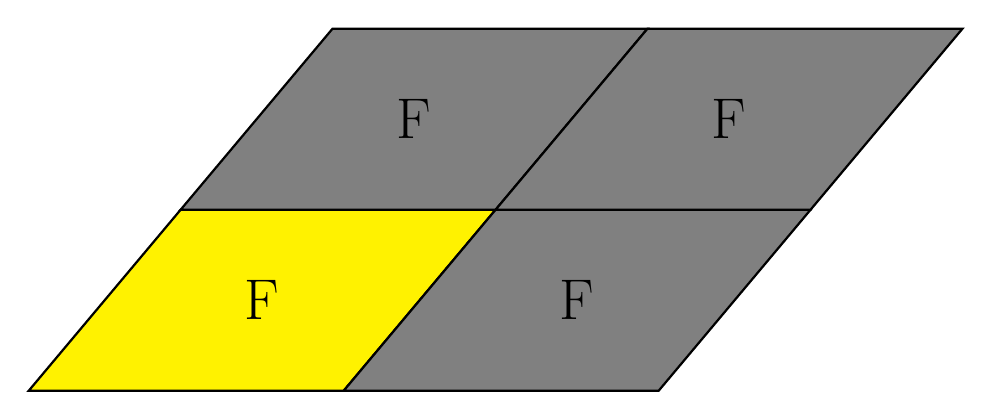
\begin{tikzpicture}
    % Define the lengths of the sides and the angle
    \def\a{4}  % length of side a
    \def\b{3}  % length of side b
    \def\angle{50}  % angle between sides a and b
    \def\s{F} % Label in center of cells

    % Calculate the coordinates of the points
    \coordinate (C00) at (0, 0);
    \coordinate (C10) at (\a, 0);
    \coordinate (C11) at ({\a + \b*cos(\angle)}, {\b * sin(\angle)});
    \coordinate (C01) at ({\b * cos(\angle)}, {\b * sin(\angle)});
    \coordinate (C02) at ({2*\b*cos(\angle)}, {2*\b * sin(\angle)});
    \coordinate (C12) at ({\a +2*\b * cos(\angle)}, {2*\b * sin(\angle)});
    \coordinate (C22) at ({2*\a + 2*\b * cos(\angle)}, {2*\b * sin(\angle)});
    \coordinate (C21) at ({2*\a + \b*cos(\angle)}, {\b * sin(\angle)});
    \coordinate (C20) at ({2*\a}, 0);

        
    % Draw the oblique unit cell
    \draw[thick,fill=yellow] (C00) -- (C10) -- (C11) -- (C01) -- cycle;
    \draw[thick,fill=gray] (C01) -- (C11) -- (C12) -- (C02) -- cycle;
    \draw[thick,fill=gray] (C10) -- (C20) -- (C21) -- (C11) -- cycle;
    \draw[thick,fill=gray] (C11) -- (C21) -- (C22) -- (C12) -- cycle;

    % Center symbols
    \node at ($(C00)!0.5!(C11)$) {\huge \s};
    \node at ($(C20)!0.5!(C11)$) {\huge \s};
    \node at ($(C02)!0.5!(C11)$) {\huge \s};
    \node at ($(C22)!0.5!(C11)$) {\huge \s};
\end{tikzpicture}
\end{document}}
        \caption*{p1}
    \end{minipage}
    \hfill
    \begin{minipage}{0.14\textwidth}
        \centering
        \scalebox{0.10}{\documentclass[class=article, crop=false]{standalone}
\usepackage{tikz}
\usepackage{subcaption}
\usetikzlibrary{calc}
\usetikzlibrary {shapes.geometric}

\begin{document}
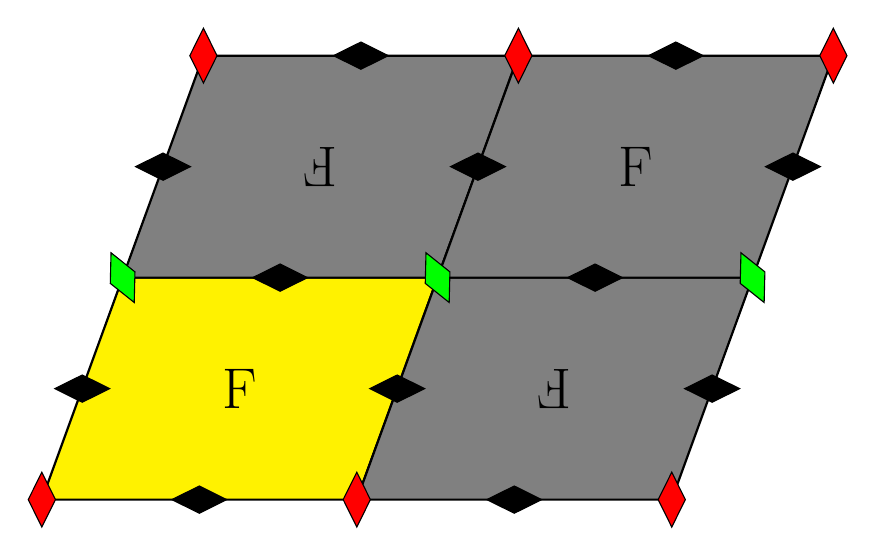
\begin{tikzpicture}
    % Define the lengths of the sides and the angle
    \def\a{4}  % length of side a
    \def\b{3}  % length of side b
    \def\angle{70}  % angle between sides a and b
    \def\s{F} % Label in center of cells

    % Calculate the coordinates of the points
    \coordinate (C00) at (0, 0);
    \coordinate (C10) at (\a, 0);
    \coordinate (C11) at ({\a + \b*cos(\angle)}, {\b * sin(\angle)});
    \coordinate (C01) at ({\b * cos(\angle)}, {\b * sin(\angle)});
    \coordinate (C02) at ({2*\b*cos(\angle)}, {2*\b * sin(\angle)});
    \coordinate (C12) at ({\a +2*\b * cos(\angle)}, {2*\b * sin(\angle)});
    \coordinate (C22) at ({2*\a + 2*\b * cos(\angle)}, {2*\b * sin(\angle)});
    \coordinate (C21) at ({2*\a + \b*cos(\angle)}, {\b * sin(\angle)});
    \coordinate (C20) at ({2*\a}, 0);
        
    % Draw the oblique unit cell
    \draw[thick,fill=yellow] (C00) -- (C10) -- (C11) -- (C01) -- cycle;
    \draw[thick,fill=gray] (C10) -- (C20) -- (C21) -- (C11) -- cycle;
    \draw[thick,fill=gray] (C01) -- (C11) -- (C12) -- (C02) -- cycle;
    \draw[thick,fill=gray] (C11) -- (C21) -- (C22) -- (C12) -- cycle;
    
    % Draw chiral center
    \node at ($(C00)!0.5!(C11)$) {\huge \s};
    \node[rotate=180] at ($(C01)!0.5!(C12)$) {\huge \s};
    \node at ($(C11)!0.5!(C22)$) {\huge \s};
    \node[rotate=180] at ($(C10)!0.5!(C21)$) {\huge \s};

    % Draw node reflections
    \draw (C00)  node[shape aspect=0.5,diamond,draw,fill=red] {};
    \draw (C10)  node[shape aspect=0.5,diamond,draw,fill=red] {};
    \draw (C20)  node[shape aspect=0.5,diamond,draw,fill=red] {};
    \draw (C01)  node[rotate = \angle-45,shape aspect=0.5,diamond,draw,fill=green] {};
    \draw (C11)  node[rotate = \angle-45,shape aspect=0.5,diamond,draw,fill=green] {};
    \draw (C21)  node[rotate = \angle-45,shape aspect=0.5,diamond,draw,fill=green] {};
    \draw (C02)  node[shape aspect=0.5,diamond,draw,fill=red] {};
    \draw (C12)  node[shape aspect=0.5,diamond,draw,fill=red] {};
    \draw (C22)  node[shape aspect=0.5,diamond,draw,fill=red] {}; 
    \draw ($(C00)!0.5!(C10)$)  node[rotate=90,shape aspect=0.5,diamond,draw,fill=black] {};
    \draw ($(C10)!0.5!(C20)$)  node[rotate=90,shape aspect=0.5,diamond,draw,fill=black] {};
    \draw ($(C00)!0.5!(C01)$)  node[rotate=90,shape aspect=0.5,diamond,draw,fill=black] {};
    \draw ($(C10)!0.5!(C11)$)  node[rotate=90,shape aspect=0.5,diamond,draw,fill=black] {};
    \draw ($(C20)!0.5!(C21)$)  node[rotate=90,shape aspect=0.5,diamond,draw,fill=black] {};
    \draw ($(C01)!0.5!(C02)$)  node[rotate=90,shape aspect=0.5,diamond,draw,fill=black] {};
    
    \draw ($(C01)!0.5!(C11)$)  node[rotate=90,shape aspect=0.5,diamond,draw,fill=black] {};
    \draw ($(C11)!0.5!(C21)$)  node[rotate=90,shape aspect=0.5,diamond,draw,fill=black] {};
    
    \draw ($(C11)!0.5!(C12)$)  node[rotate=90,shape aspect=0.5,diamond,draw,fill=black] {};
    \draw ($(C21)!0.5!(C22)$)  node[rotate=90,shape aspect=0.5,diamond,draw,fill=black] {};
    \draw ($(C02)!0.5!(C12)$)  node[rotate=90,shape aspect=0.5,diamond,draw,fill=black] {};
    \draw ($(C12)!0.5!(C22)$)  node[rotate=90,shape aspect=0.5,diamond,draw,fill=black] {};
\end{tikzpicture}
\end{document}}
        \caption*{p2}
    \end{minipage}
    \hfill
    \begin{minipage}{0.10\textwidth}
        \centering
        \scalebox{0.15}{\documentclass[class=article, crop=false]{standalone}
\usepackage{tikz}
\usepackage{subcaption}
\usetikzlibrary{calc}
\usetikzlibrary {shapes.geometric}

\begin{document}
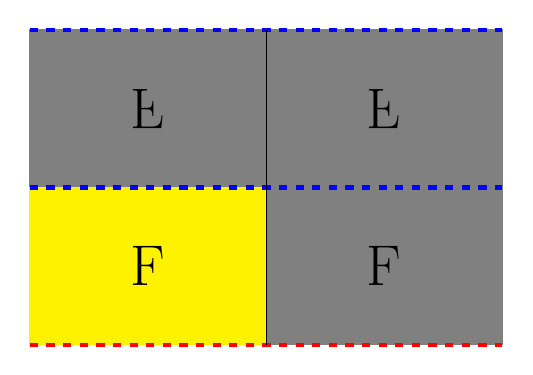
\begin{tikzpicture}
            % Define the lengths of the sides and the angle
            \def\a{3}  % length of side a
            \def\b{2}  % length of side b
            \def\angle{90}  % angle between sides a and b
            \def\s{F} % Label in center of cells

            \def\x{0.5} % Boundary 
            \def\y{0.5} % Boundary
        
            % Calculate the coordinates of the points
            \coordinate (C00) at (0, 0);
            \coordinate (C10) at (\a, 0);
            \coordinate (C11) at ({\a + \b*cos(\angle)}, {\b * sin(\angle)});
            \coordinate (C01) at ({\b * cos(\angle)}, {\b * sin(\angle)});
            \coordinate (C02) at ({2*\b*cos(\angle)}, {2*\b * sin(\angle)});
            \coordinate (C12) at ({\a +2*\b * cos(\angle)}, {2*\b * sin(\angle)});
            \coordinate (C22) at ({2*\a + 2*\b * cos(\angle)}, {2*\b * sin(\angle)});
            \coordinate (C21) at ({2*\a + \b*cos(\angle)}, {\b * sin(\angle)});
            \coordinate (C20) at ({2*\a}, 0);

            \coordinate (A1) at ($(C00)!0.6666!(C11)$);
            \coordinate (A2) at ($(C11)!0.3333!(C22)$);
        
            % Draw the oblique unit cell
            \draw[fill=gray,gray] (C00) -- (C20) -- (C22) -- (C02) -- cycle;
            \draw[fill=yellow,yellow] (C00) -- (C10) -- (C11) -- (C01) -- cycle;


            % Draw mirror lines
            \draw[ultra thick,blue,dashed] (C01) -- (C21);
            \draw[ultra thick,red,dashed] (C00) -- (C20);
            \draw[ultra thick,blue,dashed] (C02) -- (C22);
            \draw[] (C10) -- (C12);
            
           
            
            % Draw chiral center
            \node at ($(C00)!0.5!(C11)$) {\huge F};
            \node[rotate=180] at ($(C01)!0.5!(C12)$) {\reflectbox{\huge F}};
            \node at ($(C10)!0.5!(C21)$) {\huge F};
            \node[rotate=180] at ($(C11)!0.5!(C22)$) {\reflectbox{\huge F}};

            
        \end{tikzpicture}
\end{document}}
        \caption*{pm}
    \end{minipage}
    \hfill
    \begin{minipage}{0.10\textwidth}
        \centering
        \scalebox{0.10}{\documentclass[class=article, crop=false]{standalone}
\usepackage{tikz}
\usepackage{subcaption}
\usetikzlibrary{calc}
\usetikzlibrary {shapes.geometric}

\begin{document}
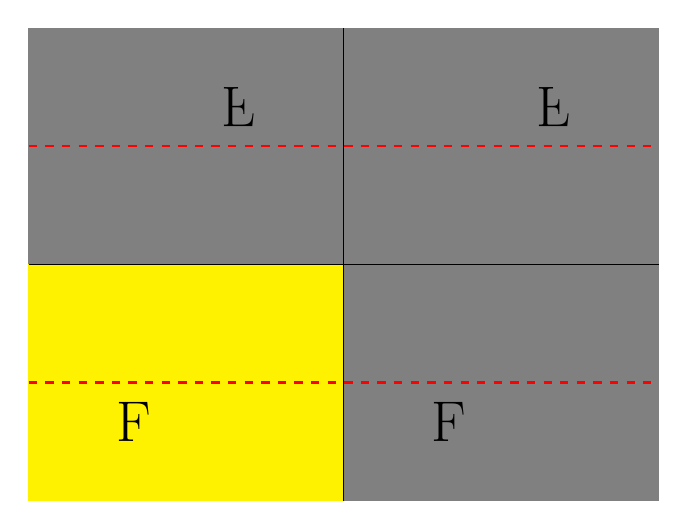
\begin{tikzpicture}
            % Define the lengths of the sides and the angle
            \def\a{4}  % length of side a
            \def\b{3}  % length of side b
            \def\angle{90}  % angle between sides a and b
            \def\s{F} % Label in center of cells


        
            % Calculate the coordinates of the points
            \coordinate (C00) at (0, 0);
            \coordinate (C10) at (\a, 0);
            \coordinate (C11) at ({\a + \b*cos(\angle)}, {\b * sin(\angle)});
            \coordinate (C01) at ({\b * cos(\angle)}, {\b * sin(\angle)});
            \coordinate (C02) at ({2*\b*cos(\angle)}, {2*\b * sin(\angle)});
            \coordinate (C12) at ({\a +2*\b * cos(\angle)}, {2*\b * sin(\angle)});
            \coordinate (C22) at ({2*\a + 2*\b * cos(\angle)}, {2*\b * sin(\angle)});
            \coordinate (C21) at ({2*\a + \b*cos(\angle)}, {\b * sin(\angle)});
            \coordinate (C20) at ({2*\a}, 0);

            \coordinate (A1) at ($(C00)!0.6666!(C11)$);
            \coordinate (A2) at ($(C11)!0.3333!(C22)$);
        
            % Draw the oblique unit cell
            \draw[fill=gray,gray] (C00) -- (C20) -- (C22) -- (C02) -- cycle;
            \draw[fill=yellow,yellow] (C00) -- (C01) -- (C11) -- (C10) -- cycle;
            \draw[] (C01) -- (C11) -- (C12);
            \draw[] (C10) -- (C11) -- (C21);
            
            % Draw chiral center
            \node at ($(C00)!0.3333!(C11)$) {\huge \s};
            \node at ($(C10)!0.3333!(C21)$) {\huge \s};
            \node[rotate=180] at ($(C11)!0.6666!(C22)$) {\reflectbox{\huge \s}};
            \node[rotate=180] at ($(C01)!0.6666!(C12)$) {\reflectbox{\huge \s}};

            % Draw mirror lines
            \draw[thick,dashed,red] ($(C00)!0.5!(C01)$) -- ($(C20)!0.5!(C21)$);
            \draw[thick,dashed,red] ($(C01)!0.5!(C02)$) -- ($(C21)!0.5!(C22)$);

            
        \end{tikzpicture}
\end{document}}
        \caption*{pg}
    \end{minipage}
    \hfill
    \begin{minipage}{0.15\textwidth}
        \centering
        \scalebox{0.10}{\documentclass[class=article, crop=false]{standalone}
\usepackage{tikz}
\usepackage{subcaption}
\usetikzlibrary{calc}
\usetikzlibrary {shapes.geometric}

\begin{document}
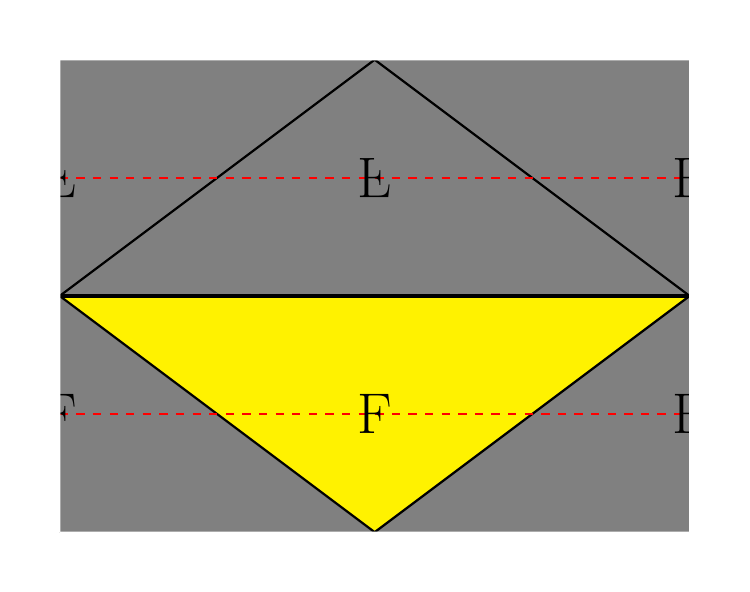
\begin{tikzpicture}
    % Define the lengths of the sides and the angle
    \def\a{4}  % length of side a
    \def\b{3}  % length of side b
    \def\angle{90}  % angle between sides a and b
    \def\s{F} % Label in center of cells

    \def\x{0.4}
    \def\y{0.4}

    % Calculate the coordinates of the points
    \coordinate (C00) at (0, 0);
    \coordinate (C10) at (\a, 0);
    \coordinate (C11) at ({\a + \b*cos(\angle)}, {\b * sin(\angle)});
    \coordinate (C01) at ({\b * cos(\angle)}, {\b * sin(\angle)});
    \coordinate (C02) at ({2*\b*cos(\angle)}, {2*\b * sin(\angle)});
    \coordinate (C12) at ({\a +2*\b * cos(\angle)}, {2*\b * sin(\angle)});
    \coordinate (C22) at ({2*\a + 2*\b * cos(\angle)}, {2*\b * sin(\angle)});
    \coordinate (C21) at ({2*\a + \b*cos(\angle)}, {\b * sin(\angle)});
    \coordinate (C20) at ({2*\a}, 0);

        
    % Draw the oblique unit cell
    \draw[fill=gray,gray] (C00) -- (C20) -- (C22) -- (C02) -- cycle;
    \draw[fill=yellow,yellow] (C10) -- (C21) -- (C01) -- cycle;

    % Draw mirror lines
    \draw[ultra thick] (C01) -- (C21);
    \draw[thick] (C10) -- (C21) -- (C12) -- (C01) -- cycle;
    \draw[thick,dashed,red] ($(C00)!0.5!(C01)$) -- ($(C20)!0.5!(C21)$);
    \draw[thick,dashed,red] ($(C01)!0.5!(C02)$) -- ($(C21)!0.5!(C22)$);

    

    % Draw boundary centre symbols
    \node at ($(C00)!0.5!(C01)$) {\huge \s};
    \node[rotate=180] at ($(C01)!0.5!(C02)$) {\reflectbox{\huge \s}};
    \node at ($(C20)!0.5!(C21)$) {\huge \s};
    \node[rotate=180] at ($(C21)!0.5!(C22)$) {\reflectbox{\huge \s}};

    % Create white border
    \draw[fill=white,white] ($(C00)-(\x,\y)$) -- ($(C20)-(-\x,\y)$) -- (C20) -- (C00);
    \draw[fill=white,white] ($(C00)-(\x,-\y)$) -- ($(C02)-(\x,-\y)$) -- (C02) -- (C00);
    \draw[fill=white,white] ($(C02)+(\x,\y)$) -- ($(C22)-(\x,-\y)$) -- (C22) -- (C02);
    \draw[fill=white,white] ($(C20)+(\x,-\y)$) -- ($(C22)+(\x,\y)$) -- (C22) -- (C20);
    
    % Center symbols
    \node at ($(C10)!0.5!(C11)$) {\huge \s};
    \node[rotate=180] at ($(C11)!0.5!(C12)$) {\reflectbox{\huge \s}};
    
\end{tikzpicture}
\end{document}}
        \caption*{cm}
    \end{minipage}
    % Row 2
    \vfill
    \begin{minipage}{0.16\textwidth}
        \centering
        \scalebox{0.10}{\documentclass[class=article, crop=false]{standalone}
\usepackage{tikz}
\usepackage{subcaption}
\usetikzlibrary{calc}
\usetikzlibrary {shapes.geometric}

\begin{document}
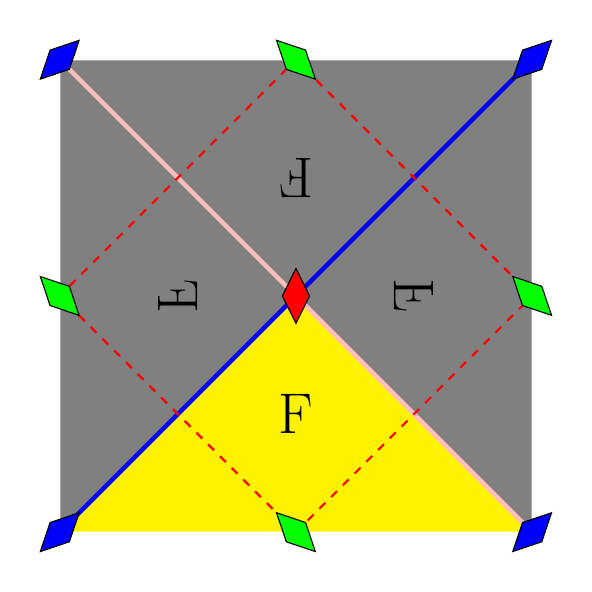
\begin{tikzpicture}
    % Define the lengths of the sides and the angle
    \def\a{3}  % length of side a
    \def\b{3}  % length of side b
    \def\angle{90}  % angle between sides a and b
    \def\s{F} % Label in center of cells

    \def\x{0.4}
    \def\y{0.4}

    % Calculate the coordinates of the points
    \coordinate (C00) at (0, 0);
    \coordinate (C10) at (\a, 0);
    \coordinate (C11) at ({\a + \b*cos(\angle)}, {\b * sin(\angle)});
    \coordinate (C01) at ({\b * cos(\angle)}, {\b * sin(\angle)});
    \coordinate (C02) at ({2*\b*cos(\angle)}, {2*\b * sin(\angle)});
    \coordinate (C12) at ({\a +2*\b * cos(\angle)}, {2*\b * sin(\angle)});
    \coordinate (C22) at ({2*\a + 2*\b * cos(\angle)}, {2*\b * sin(\angle)});
    \coordinate (C21) at ({2*\a + \b*cos(\angle)}, {\b * sin(\angle)});
    \coordinate (C20) at ({2*\a}, 0);

        
    % Draw the oblique unit cell
    \draw[fill=gray,gray] (C00) -- (C20) -- (C22) -- (C02) -- cycle;
    \draw[fill=yellow,yellow] (C00) -- (C11) -- (C20) -- cycle;

    % Draw mirror lines
    \draw[ultra thick,blue] (C00) -- (C22);
    \draw[ultra thick,pink] (C20) -- (C02);
    \draw[thick,dashed,red] (C10) -- (C21) -- (C12) -- (C01) -- cycle;
    
    

    % Draw boundary centre symbols
    %\node[rotate=180] at ($(C00)!0.5!(C01)$) {\huge \s};
    %\node[rotate=0] at ($(C01)!0.5!(C02)$) {\reflectbox{\huge \s}};
    %\node at ($(C20)!0.5!(C21)$) {\huge \s};
    %\node[rotate=180] at ($(C21)!0.5!(C22)$) {\reflectbox{\huge \s}};

    % Create white border
    \draw[fill=white,white] ($(C00)-(\x,\y)$) -- ($(C20)-(-\x,\y)$) -- (C20) -- (C00);
    \draw[fill=white,white] ($(C00)-(\x,-\y)$) -- ($(C02)-(\x,-\y)$) -- (C02) -- (C00);
    \draw[fill=white,white] ($(C02)+(\x,\y)$) -- ($(C22)-(\x,-\y)$) -- (C22) -- (C02);
    \draw[fill=white,white] ($(C20)+(\x,-\y)$) -- ($(C22)+(\x,\y)$) -- (C22) -- (C20);
    
    % Center symbols
    \node at ($(C10)!0.5!(C11)$) {\huge \s};
    \node[rotate=270] at ($(C01)!0.5!(C11)$) {\reflectbox{\huge \s}};
    \node[rotate=180] at ($(C12)!0.5!(C11)$) {\huge \s};
    \node[rotate=90] at ($(C21)!0.5!(C11)$) {\reflectbox{\huge \s}};

    % Draw node rotations
    \draw (C11)  node[rotate = 0,shape aspect=0.5,diamond,draw,fill=red] {};
    \draw (C10)  node[rotate = 45,shape aspect=0.5,diamond,draw,fill=green] {};
    \draw (C01)  node[rotate = 45,shape aspect=0.5,diamond,draw,fill=green] {};
    \draw (C21)  node[rotate = 45,shape aspect=0.5,diamond,draw,fill=green] {};
    \draw (C12)  node[rotate = 45,shape aspect=0.5,diamond,draw,fill=green] {};
    \draw (C00)  node[rotate = 135,shape aspect=0.5,diamond,draw,fill=blue] {};
    \draw (C20)  node[rotate = 135,shape aspect=0.5,diamond,draw,fill=blue] {};
    \draw (C02)  node[rotate = 135,shape aspect=0.5,diamond,draw,fill=blue] {};
    \draw (C22)  node[rotate = 135,shape aspect=0.5,diamond,draw,fill=blue] {};
    
\end{tikzpicture}
\end{document}}
        \caption*{cmm}
    \end{minipage}
    \hfill
    \begin{minipage}{0.10\textwidth}
        \centering
        \scalebox{0.10}{\documentclass[class=article, crop=false]{standalone}
\usepackage{tikz}
\usepackage{subcaption}
\usetikzlibrary{calc}
\usetikzlibrary {shapes.geometric}

\begin{document}
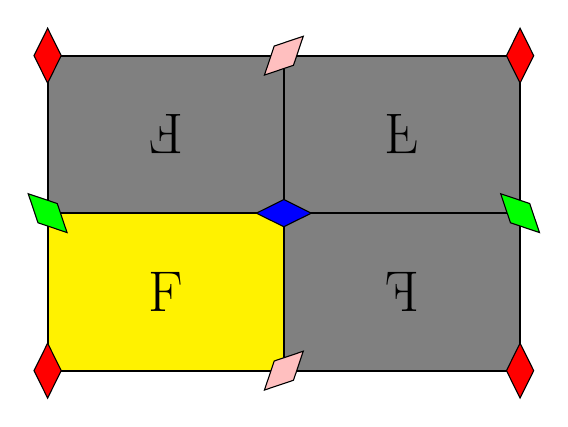
\begin{tikzpicture}
            % Define the lengths of the sides and the angle
            \def\a{3}  % length of side a
            \def\b{2}  % length of side b
            \def\angle{90}  % angle between sides a and b
            \def\s{F}

        
            % Calculate the coordinates of the points
            \coordinate (C00) at (0, 0);
            \coordinate (C10) at (\a, 0);
            \coordinate (C11) at ({\a + \b*cos(\angle)}, {\b * sin(\angle)});
            \coordinate (C01) at ({\b * cos(\angle)}, {\b * sin(\angle)});
            \coordinate (C02) at ({2*\b*cos(\angle)}, {2*\b * sin(\angle)});
            \coordinate (C12) at ({\a +2*\b * cos(\angle)}, {2*\b * sin(\angle)});
            \coordinate (C22) at ({2*\a + 2*\b * cos(\angle)}, {2*\b * sin(\angle)});
            \coordinate (C21) at ({2*\a + \b*cos(\angle)}, {\b * sin(\angle)});
            \coordinate (C20) at ({2*\a}, 0);
        
            % Draw the oblique unit cell
            \draw[thick,fill=yellow] (C00) -- (C01) -- (C11) -- (C10) -- cycle;
            \draw[thick,fill=gray] (C01) -- (C11) -- (C12) -- (C02) -- cycle;
            
            \draw[thick,fill=gray] (C11) -- (C12) -- (C22) -- (C21) -- cycle;
            \draw[thick,fill=gray] (C10) -- (C20) -- (C21) -- (C11) -- cycle;
            
            % Draw chiral center
            \node at ($(C00)!0.5!(C11)$) {\huge \s};
            \node[rotate=180] at ($(C01)!0.5!(C12)$) {\huge \s};
            \node at ($(C10)!0.5!(C21)$) {\reflectbox{\huge \s}};
            \node[rotate=180] at ($(C11)!0.5!(C22)$) {\reflectbox{\huge \s}};

            % Draw node reflections
            \draw (C00)  node[shape aspect=0.5,diamond,draw,fill=red] {};
            \draw (C10)  node[shape aspect=0.5,rotate=-45,diamond,draw,fill=pink] {};
            \draw (C11)  node[rotate = \angle,shape aspect=0.5,diamond,draw,fill=blue] {};
            \draw (C01)  node[shape aspect=0.5,rotate=45,diamond,draw,fill=green] {};
            \draw (C02)  node[shape aspect=0.5,diamond,draw,fill=red] {};
            \draw (C12)  node[shape aspect=0.5,rotate=-45,diamond,draw,fill=pink] {};
            \draw (C22)  node[shape aspect=0.5,diamond,draw,fill=red] {};
            \draw (C21)  node[shape aspect=0.5,rotate=45,diamond,draw,fill=green] {};
            \draw (C20)  node[shape aspect=0.5,diamond,draw,fill=red] {};

            %\draw ($(A)!0.5!(E)$) node[shape aspect=0.5,diamond,draw,fill=black] {};
            
        \end{tikzpicture}
\end{document}}
        \caption*{pmm}
    \end{minipage}
    \hfill
    \begin{minipage}{0.16\textwidth}
        \centering
        \scalebox{0.15}{\documentclass[class=article, crop=false]{standalone}
\usepackage{tikz}
\usepackage{subcaption}
\usetikzlibrary{calc}
\usetikzlibrary {shapes.geometric}

\begin{document}
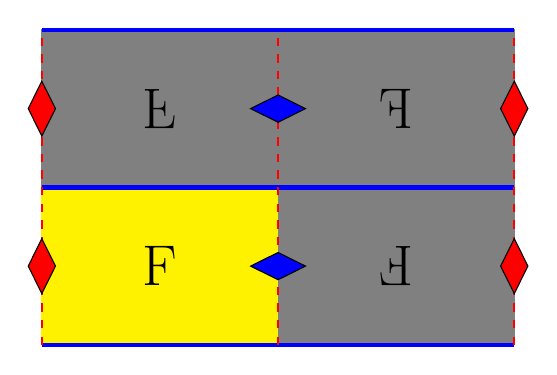
\begin{tikzpicture}
            % Define the lengths of the sides and the angle
            \def\a{3}  % length of side a
            \def\b{2}  % length of side b
            \def\angle{90}  % angle between sides a and b
            \def\s{F}
        
            % Calculate the coordinates of the points
            \coordinate (C00) at (0, 0);
            \coordinate (C10) at (\a, 0);
            \coordinate (C11) at ({\a + \b*cos(\angle)}, {\b * sin(\angle)});
            \coordinate (C01) at ({\b * cos(\angle)}, {\b * sin(\angle)});
            \coordinate (C02) at ({2*\b*cos(\angle)}, {2*\b * sin(\angle)});
            \coordinate (C12) at ({\a +2*\b * cos(\angle)}, {2*\b * sin(\angle)});
            \coordinate (C22) at ({2*\a + 2*\b * cos(\angle)}, {2*\b * sin(\angle)});
            \coordinate (C21) at ({2*\a + \b*cos(\angle)}, {\b * sin(\angle)});
            \coordinate (C20) at ({2*\a}, 0);
        
            % Draw the oblique unit cell
            \draw[fill=yellow,yellow] (C00) -- (C01) -- (C11) -- (C10) -- cycle;
            \draw[fill=gray,gray] (C01) -- (C11) -- (C12) -- (C02) -- cycle;
            
            \draw[fill=gray,gray] (C11) -- (C12) -- (C22) -- (C21) -- cycle;
            \draw[fill=gray,gray] (C10) -- (C20) -- (C21) -- (C11) -- cycle;

            % Draw mirror lines
            \draw[ultra thick,blue] (C00) -- (C20);
            \draw[ultra thick,blue] (C01) -- (C21);
            \draw[ultra thick,blue] (C02) -- (C22);
            \draw[thick,dashed,red] (C00) -- (C02);
            \draw[thick,dashed,red] (C10) -- (C12);
            \draw[thick,dashed,red] (C20) -- (C22);
            
            % Draw chiral center
            \node at ($(C00)!0.5!(C11)$) {\huge \s};
            \node[rotate=180] at ($(C01)!0.5!(C12)$) {\reflectbox{\huge \s}};
            \node[rotate=180] at ($(C10)!0.5!(C21)$) {\huge \s};
            \node[rotate=0] at ($(C11)!0.5!(C22)$) {\reflectbox{\huge \s}};

            % Draw node rotations
            \draw ($(C00)!0.5!(C01)$)  node[shape aspect=0.5,diamond,draw,fill=red] {};
            \draw ($(C01)!0.5!(C02)$)  node[shape aspect=0.5,diamond,draw,fill=red] {};
            \draw ($(C10)!0.5!(C11)$)  node[rotate = 90,shape aspect=0.5,diamond,draw,fill=blue] {};
            \draw ($(C11)!0.5!(C12)$)  node[shape aspect=0.5,rotate=90,diamond,draw,fill=blue] {};
            \draw ($(C20)!0.5!(C21)$)  node[shape aspect=0.5,diamond,draw,fill=red] {};
            \draw ($(C21)!0.5!(C22)$)  node[shape aspect=0.5,diamond,draw,fill=red] {};
            
        \end{tikzpicture}
\end{document}}
        \caption*{pmg}
    \end{minipage}
    \hfill
    \begin{minipage}{0.16\textwidth}
        \centering
        \scalebox{0.15}{\documentclass[class=article, crop=false]{standalone}
\usepackage{tikz}
\usepackage{subcaption}
\usetikzlibrary{calc}
\usetikzlibrary {shapes.geometric}

\begin{document}
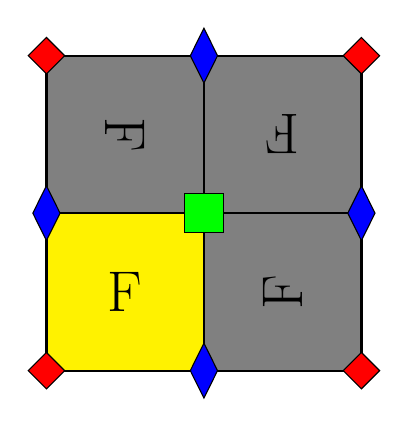
\begin{tikzpicture}
            % Define the lengths of the sides and the angle
            \def\a{2}  % length of side a
            \def\b{2}  % length of side b
            \def\angle{90}  % angle between sides a and b
            \def\s{F}
        
            % Calculate the coordinates of the points
            \coordinate (C00) at (0, 0);
            \coordinate (C10) at (\a, 0);
            \coordinate (C11) at ({\a + \b*cos(\angle)}, {\b * sin(\angle)});
            \coordinate (C01) at ({\b * cos(\angle)}, {\b * sin(\angle)});
            \coordinate (C02) at ({2*\b*cos(\angle)}, {2*\b * sin(\angle)});
            \coordinate (C12) at ({\a +2*\b * cos(\angle)}, {2*\b * sin(\angle)});
            \coordinate (C22) at ({2*\a + 2*\b * cos(\angle)}, {2*\b * sin(\angle)});
            \coordinate (C21) at ({2*\a + \b*cos(\angle)}, {\b * sin(\angle)});
            \coordinate (C20) at ({2*\a}, 0);
        
            % Draw the oblique unit cell
            \draw[thick,fill=yellow] (C00) -- (C01) -- (C11) -- (C10) -- cycle;
            \draw[thick,fill=gray] (C01) -- (C11) -- (C12) -- (C02) -- cycle;
            
            \draw[thick,fill=gray] (C11) -- (C12) -- (C22) -- (C21) -- cycle;
            \draw[thick,fill=gray] (C10) -- (C20) -- (C21) -- (C11) -- cycle;
            
            % Draw chiral center
            \node at ($(C00)!0.5!(C11)$) {\huge \s};
            \node[rotate=-90] at ($(C01)!0.5!(C12)$) {\huge \s};
            \node[rotate=90] at ($(C10)!0.5!(C21)$) {\huge \s};
            \node[rotate=180] at ($(C11)!0.5!(C22)$) {\huge \s};

            % Draw node reflections and rotations
            \draw (C00)  node[shape aspect=1,diamond,draw,fill=red] {};
            \draw (C10)  node[shape aspect=0.5,diamond,draw,fill=blue] {};
            \draw (C11)  node[minimum size=0.5cm,draw,fill=green] {};
            \draw (C01)  node[shape aspect=0.5,diamond,draw,fill=blue] {};
            \draw (C02)  node[shape aspect=1,diamond,draw,fill=red] {};
            \draw (C12)  node[shape aspect=0.5,diamond,draw,fill=blue] {};
            \draw (C22)  node[shape aspect=1,diamond,draw,fill=red] {};
            \draw (C21)  node[shape aspect=0.5,diamond,draw,fill=blue] {};
            \draw (C20)  node[shape aspect=1,diamond,draw,fill=red] {};

            %\draw ($(A)!0.5!(E)$) node[shape aspect=0.5,diamond,draw,fill=black] {};
            
        \end{tikzpicture}
\end{document}}
        \caption*{p4}
    \end{minipage}
    \vfill
    % Row 3
    \begin{minipage}{0.10\textwidth}
        \centering
        \scalebox{0.10}{\documentclass[class=article, crop=false]{standalone}
\usepackage{tikz}
\usepackage{subcaption}
\usetikzlibrary{calc}
\usetikzlibrary {shapes.geometric}

\begin{document}
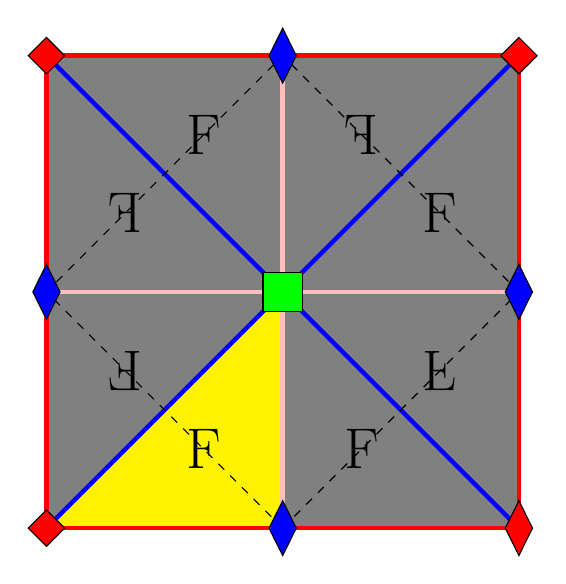
\begin{tikzpicture}
            % Define the lengths of the sides and the angle
            \def\a{3}  % length of side a
            \def\b{3}  % length of side b
            \def\angle{90}  % angle between sides a and b
            \def\s{F}
        
            % Calculate the coordinates of the points
            \coordinate (C00) at (0, 0);
            \coordinate (C10) at (\a, 0);
            \coordinate (C11) at ({\a + \b*cos(\angle)}, {\b * sin(\angle)});
            \coordinate (C01) at ({\b * cos(\angle)}, {\b * sin(\angle)});
            \coordinate (C02) at ({2*\b*cos(\angle)}, {2*\b * sin(\angle)});
            \coordinate (C12) at ({\a +2*\b * cos(\angle)}, {2*\b * sin(\angle)});
            \coordinate (C22) at ({2*\a + 2*\b * cos(\angle)}, {2*\b * sin(\angle)});
            \coordinate (C21) at ({2*\a + \b*cos(\angle)}, {\b * sin(\angle)});
            \coordinate (C20) at ({2*\a}, 0);
        
            % Draw the oblique unit cell
            \draw[thick,fill=gray] (C00) -- (C20) -- (C22) -- (C02) -- cycle;
            \draw[thick,fill=yellow] (C00) -- (C10) -- (C11) -- cycle;
            \draw[ultra thick,red] (C00) -- (C20) -- (C22) -- (C02) -- cycle;
            \draw[ultra thick,blue] (C11) -- (C00);
            \draw[ultra thick,blue] (C11) -- (C20);
            \draw[ultra thick,blue] (C11) -- (C22);
            \draw[ultra thick,blue] (C11) -- (C02);
            \draw[ultra thick,pink] (C11) -- (C10);
            \draw[ultra thick,pink] (C11) -- (C21);
            \draw[ultra thick,pink] (C11) -- (C12);
            \draw[ultra thick,pink] (C11) -- (C01);
            
            % Draw mirrow lines
            \draw[dashed] (C10) -- (C21) -- (C12) -- (C01) -- cycle;
            
            % Draw chiral center
            \node at ($(C01)!0.6666!(C10)$) {\huge \s};
            \node[rotate=180] at ($(C01)!0.3333!(C10)$) {\huge \s};
            \node[rotate=180] at ($(C10)!0.6666!(C21)$) {\reflectbox{\huge \s}};
            \node at ($(C10)!0.3333!(C21)$) {\huge \s};
            \node at ($(C21)!0.6666!(C12)$) {\reflectbox{\huge \s}};
            \node at ($(C21)!0.3333!(C12)$) {\huge \s};
            \node at ($(C01)!0.6666!(C12)$) {\huge \s};
            \node[rotate=0] at ($(C01)!0.3333!(C12)$) {\reflectbox{\huge \s}};

            % Draw node reflections
            \draw (C00)  node[shape aspect=1,diamond,draw,fill=red] {};
            \draw (C10)  node[shape aspect=0.5,diamond,draw,fill=blue] {};
            \draw (C11)  node[minimum size=0.5cm,draw,fill=green] {};
            \draw (C01)  node[shape aspect=0.5,diamond,draw,fill=blue] {};
            \draw (C02)  node[shape aspect=1,diamond,draw,fill=red] {};
            \draw (C12)  node[shape aspect=0.5,diamond,draw,fill=blue] {};
            \draw (C22)  node[shape aspect=1,diamond,draw,fill=red] {};
            \draw (C21)  node[shape aspect=0.5,diamond,draw,fill=blue] {};
            \draw (C20)  node[shape aspect=0.5,diamond,draw,fill=red] {};

            %\draw ($(A)!0.5!(E)$) node[shape aspect=0.5,diamond,draw,fill=black] {};
            
        \end{tikzpicture}
\end{document}}
        \caption*{p4m}
    \end{minipage}
    \hfill
     \begin{minipage}{0.10\textwidth}
        \centering
        \scalebox{0.10}{\documentclass[class=article, crop=false]{standalone}
\usepackage{tikz}
\usepackage{subcaption}
\usetikzlibrary{calc}
\usetikzlibrary {shapes.geometric}

\begin{document}
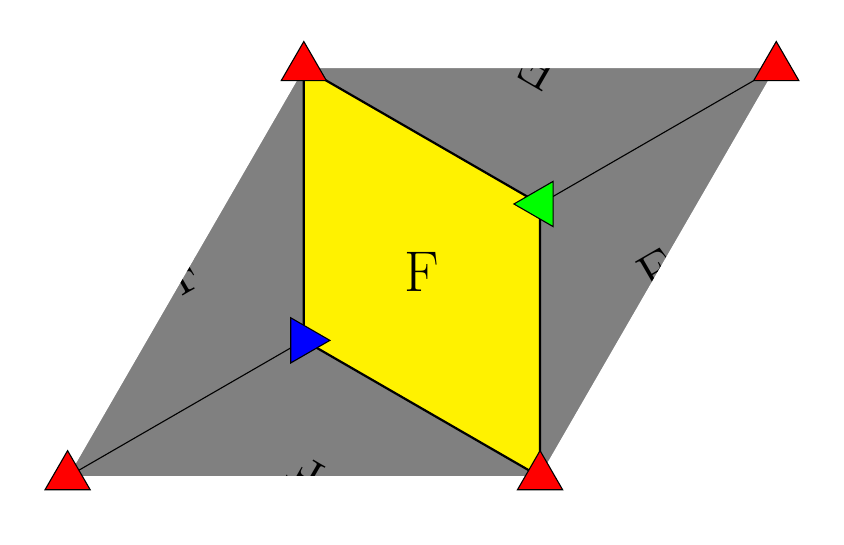
\begin{tikzpicture}
            % Define the lengths of the sides and the angle
            \def\a{3}  % length of side a
            \def\b{3}  % length of side b
            \def\angle{60}  % angle between sides a and b
            \def\s{F} % Label in center of cells

            \def\x{0.5} % Boundary 
            \def\y{0.5} % Boundary

        
            % Calculate the coordinates of the points
            \coordinate (C00) at (0, 0);
            \coordinate (C10) at (\a, 0);
            \coordinate (C11) at ({\a + \b*cos(\angle)}, {\b * sin(\angle)});
            \coordinate (C01) at ({\b * cos(\angle)}, {\b * sin(\angle)});
            \coordinate (C02) at ({2*\b*cos(\angle)}, {2*\b * sin(\angle)});
            \coordinate (C12) at ({\a +2*\b * cos(\angle)}, {2*\b * sin(\angle)});
            \coordinate (C22) at ({2*\a + 2*\b * cos(\angle)}, {2*\b * sin(\angle)});
            \coordinate (C21) at ({2*\a + \b*cos(\angle)}, {\b * sin(\angle)});
            \coordinate (C20) at ({2*\a}, 0);
        
            % Draw the oblique unit cell
            \draw[fill=gray,gray] (C00) -- (C20) -- (C22) -- (C02) -- cycle;
            \draw[thick,fill=yellow] ($(C00)!0.6666!(C11)$) -- (C20) -- ($(C11)!0.3333!(C22)$) -- (C02) -- cycle;

            
            % Draw boundary chiral centres
            \node[rotate=150] at (C10) {\huge \s};
            \node[rotate=30] at (C21) {\huge \s};
            \node[rotate=150] at (C12) {\huge \s};
            \node[rotate=30] at (C01) {\huge \s};

            % Create white border
            \draw[fill=white,white] ($(C00)-(\x,\y)$) -- ($(C20)-(-\x,\y)$) -- (C20) -- (C00);
            \draw[fill=white,white] ($(C00)-(\x,-\y)$) -- ($(C02)-(\x,-\y)$) -- (C02) -- (C00);
            \draw[fill=white,white] ($(C02)+(\x,\y)$) -- ($(C22)-(\x,-\y)$) -- (C22) -- (C02);
            \draw[fill=white,white] ($(C20)+(\x,-\y)$) -- ($(C22)+(\x,\y)$) -- (C22) -- (C20);

            % Draw chiral inner centre
            \node at (C11) {\huge \s};


            % Draw mirrow lines
            \draw (C00) -- ($(C00)!0.6666!(C11)$);
            \draw ($(C11)!0.3333!(C22)$) -- (C22);


            % Draw node reflections
            \draw (C00)  node[regular polygon, regular polygon sides=3, draw, fill=red, minimum size=0.5cm] {};
            \draw (C02)  node[regular polygon, regular polygon sides=3, draw, fill=red, minimum size=0.5cm] {};
            \draw (C22)  node[regular polygon, regular polygon sides=3, draw, fill=red, minimum size=0.5cm] {};
            \draw (C20)  node[regular polygon, regular polygon sides=3, draw, fill=red, minimum size=0.5cm] {};

            \draw ($(C00)!0.6666!(C11)$)  node[rotate = 30,regular polygon, regular polygon sides=3, draw, fill=blue, minimum size=0.5cm] {};
            \draw ($(C11)!0.3333!(C22)$)  node[rotate=90, regular polygon, regular polygon sides=3, draw, fill=green, minimum size=0.5cm] {};    
        \end{tikzpicture}
\end{document}}
        \caption*{p3}
    \end{minipage}
    \hfill
    \begin{minipage}{0.16\textwidth}
        \centering
        \scalebox{0.10}{\documentclass[class=article, crop=false]{standalone}
\usepackage{tikz}
\usepackage{subcaption}
\usetikzlibrary{calc}
\usetikzlibrary {shapes.geometric}

\begin{document}
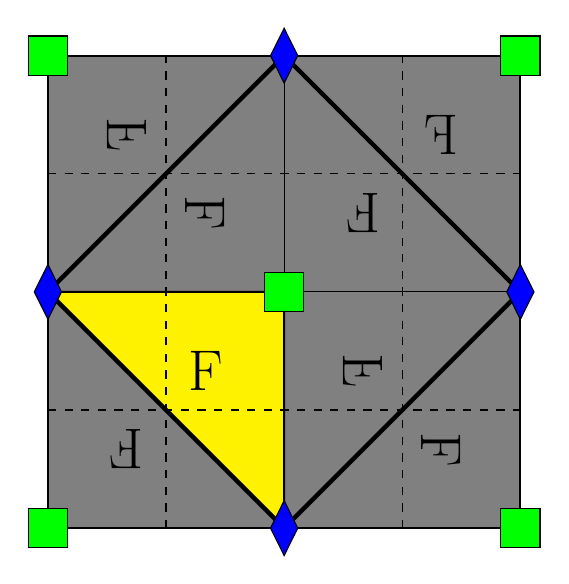
\begin{tikzpicture}
            % Define the lengths of the sides and the angle
            \def\a{3}  % length of side a
            \def\b{3}  % length of side b
            \def\angle{90}  % angle between sides a and b
            \def\s{F}
        
            % Calculate the coordinates of the points
            \coordinate (C00) at (0, 0);
            \coordinate (C10) at (\a, 0);
            \coordinate (C11) at ({\a + \b*cos(\angle)}, {\b * sin(\angle)});
            \coordinate (C01) at ({\b * cos(\angle)}, {\b * sin(\angle)});
            \coordinate (C02) at ({2*\b*cos(\angle)}, {2*\b * sin(\angle)});
            \coordinate (C12) at ({\a +2*\b * cos(\angle)}, {2*\b * sin(\angle)});
            \coordinate (C22) at ({2*\a + 2*\b * cos(\angle)}, {2*\b * sin(\angle)});
            \coordinate (C21) at ({2*\a + \b*cos(\angle)}, {\b * sin(\angle)});
            \coordinate (C20) at ({2*\a}, 0);
        
            % Draw the oblique unit cell
            \draw[thick,fill=gray] (C00) -- (C20) -- (C22) -- (C02) -- cycle;
            \draw[thick,fill=yellow] (C01) -- (C10) -- (C11) -- cycle;
            \draw[ultra thick] (C10) -- (C21) -- (C12) -- (C01) -- cycle;

            
            % Draw mirrow lines
            \draw[dashed] ($(C00)!0.5!(C10)$) -- ($(C02)!0.5!(C12)$);
            \draw[thin] (C10) -- (C12);
            \draw[dashed] ($(C10)!0.5!(C20)$) -- ($(C12)!0.5!(C22)$);
            \draw[dashed] ($(C00)!0.5!(C01)$) -- ($(C20)!0.5!(C21)$);
            \draw[thin] (C01) -- (C21);
            \draw[dashed] ($(C01)!0.5!(C02)$) -- ($(C21)!0.5!(C22)$);
            
            % Draw chiral center
            \node[rotate=180] at ($(C11)!0.6666!(C00)$) {\huge \s};
            \node at ($(C11)!0.3333!(C00)$) {\huge \s};
            \node[rotate=90] at ($(C11)!0.6666!(C02)$) {\reflectbox{\huge \s}};
            \node[rotate=-90] at ($(C11)!0.3333!(C02)$) {\huge \s};
            \node at ($(C11)!0.6666!(C22)$) {\reflectbox{\huge \s}};
            \node[rotate=180] at ($(C11)!0.3333!(C22)$) {\huge \s};
            \node[rotate=-90] at ($(C11)!0.6666!(C20)$) {\huge \s};
            \node[rotate=90] at ($(C11)!0.3333!(C20)$) {\reflectbox{\huge 
            \s}};

            % Draw node reflections
            \draw (C00)  node[minimum size=0.5cm,draw,fill=green] {};
            \draw (C10)  node[shape aspect=0.5,diamond,draw,fill=blue] {};
            \draw (C11)  node[minimum size=0.5cm,draw,fill=green] {};
            \draw (C01)  node[shape aspect=0.5,diamond,draw,fill=blue] {};
            \draw (C02)  node[minimum size=0.5cm,draw,fill=green] {};
            \draw (C12)  node[shape aspect=0.5,diamond,draw,fill=blue] {};
            \draw (C22)  node[minimum size=0.5cm,draw,fill=green] {};
            \draw (C21)  node[shape aspect=0.5,diamond,draw,fill=blue] {};
            \draw (C20)  node[minimum size=0.5cm,draw,fill=green] {};

            %\draw ($(A)!0.5!(E)$) node[shape aspect=0.5,diamond,draw,fill=black] {};
            
        \end{tikzpicture}
\end{document}}
        \caption*{p4g}
    \end{minipage}
    \hfill
    \begin{minipage}{0.10\textwidth}
        \centering
        \scalebox{0.13}{\documentclass[class=article, crop=false]{standalone}
\usepackage{tikz}
\usepackage{subcaption}
\usetikzlibrary{calc}
\usetikzlibrary {shapes.geometric}

\begin{document}
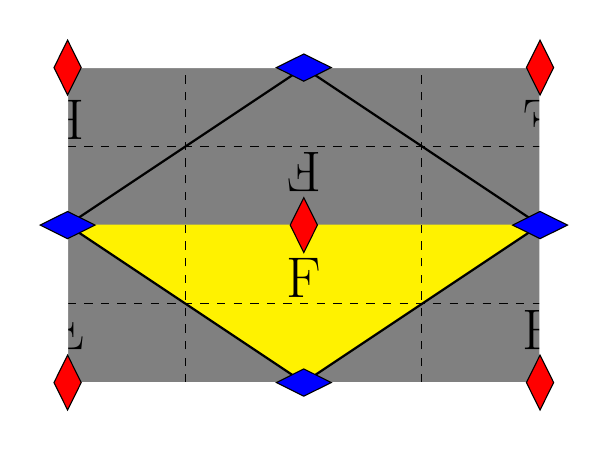
\begin{tikzpicture}
            % Define the lengths of the sides and the angle
            \def\a{3}  % length of side a
            \def\b{2}  % length of side b
            \def\angle{90}  % angle between sides a and b
            \def\s{F}

            \def\x{0.5} % Boundary 
            \def\y{0.5} % Boundary
        
            % Calculate the coordinates of the points
            \coordinate (C00) at (0, 0);
            \coordinate (C10) at (\a, 0);
            \coordinate (C11) at ({\a + \b*cos(\angle)}, {\b * sin(\angle)});
            \coordinate (C01) at ({\b * cos(\angle)}, {\b * sin(\angle)});
            \coordinate (C02) at ({2*\b*cos(\angle)}, {2*\b * sin(\angle)});
            \coordinate (C12) at ({\a +2*\b * cos(\angle)}, {2*\b * sin(\angle)});
            \coordinate (C22) at ({2*\a + 2*\b * cos(\angle)}, {2*\b * sin(\angle)});
            \coordinate (C21) at ({2*\a + \b*cos(\angle)}, {\b * sin(\angle)});
            \coordinate (C20) at ({2*\a}, 0);
        
            % Draw the oblique unit cell
            \draw[fill=gray,gray] (C00) -- (C20) -- (C22) -- (C02) -- cycle;
            \draw[fill=yellow,yellow] (C01) -- (C10) -- (C21) -- cycle;
            \draw[thick] (C10) -- (C21) -- (C12) -- (C01) -- cycle;
            
            % Draw mirrow lines
            \draw[dashed] ($(C00)!0.5!(C01)$) -- ($(C20)!0.5!(C21)$);
            \draw[dashed] ($(C01)!0.5!(C02)$) -- ($(C21)!0.5!(C22)$);
            \draw[dashed] ($(C00)!0.5!(C10)$) -- ($(C02)!0.5!(C12)$);
            \draw[dashed] ($(C10)!0.5!(C20)$) -- ($(C12)!0.5!(C22)$);


            % Draw inner centres
            \node at ($(C01)!0.6666!(C02)$) {\reflectbox{\huge \s}};
            \node[rotate=180] at ($(C00)!0.3333!(C01)$) {\reflectbox{\huge \s}};
            \node at ($(C21)!0.6666!(C22)$) {\reflectbox{\huge \s}};
            \node[rotate=180] at ($(C20)!0.3333!(C21)$) {\reflectbox{\huge \s}};

            % Create white border
            \draw[fill=white,white] ($(C00)-(\x,\y)$) -- ($(C20)-(-\x,\y)$) -- (C20) -- (C00);
            \draw[fill=white,white] ($(C00)-(\x,-\y)$) -- ($(C02)-(\x,-\y)$) -- (C02) -- (C00);
            \draw[fill=white,white] ($(C02)+(\x,\y)$) -- ($(C22)-(\x,-\y)$) -- (C22) -- (C02);
            \draw[fill=white,white] ($(C20)+(\x,-\y)$) -- ($(C22)+(\x,\y)$) -- (C22) -- (C20);
            
            % Draw chiral center
            \node at ($(C10)!0.6666!(C11)$) {\huge \s};
            \node[rotate=180] at ($(C11)!0.3333!(C12)$) {\huge \s};
            

            % Draw node reflections
            \draw (C00)  node[shape aspect=0.5,diamond,draw,fill=red] {};
            \draw (C10)  node[shape aspect=0.5,rotate=90,diamond,draw,fill=blue] {};
            \draw (C11)  node[shape aspect=0.5,diamond,draw,fill=red] {};
            \draw (C01)  node[shape aspect=0.5,rotate=90,diamond,draw,fill=blue] {};
            \draw (C02)  node[shape aspect=0.5,diamond,draw,fill=red] {};
            \draw (C12)  node[shape aspect=0.5,rotate=90,diamond,draw,fill=blue] {};
            \draw (C22)  node[shape aspect=0.5,diamond,draw,fill=red] {};
            \draw (C21)  node[shape aspect=0.5,rotate=90,diamond,draw,fill=blue] {};
            \draw (C20)  node[shape aspect=0.5,diamond,draw,fill=red] {};
        \end{tikzpicture}
\end{document}}
        \caption*{pgg}
    \end{minipage}
    % Row 4
    \vfill
    \begin{minipage}{0.10\textwidth}
        \centering
        \scalebox{0.10}{\documentclass[class=article, crop=false]{standalone}
\usepackage{tikz}
\usepackage{subcaption}
\usetikzlibrary{calc}
\usetikzlibrary {shapes.geometric}

\begin{document}
\begin{tikzpicture}
            % Define the lengths of the sides and the angle
            \def\a{3}  % length of side a
            \def\b{3}  % length of side b
            \def\angle{60}  % angle between sides a and b
            \def\s{F} % Label in center of cells
        
            % Calculate the coordinates of the points
            \coordinate (C00) at (0, 0);
            \coordinate (C10) at (\a, 0);
            \coordinate (C11) at ({\a + \b*cos(\angle)}, {\b * sin(\angle)});
            \coordinate (C01) at ({\b * cos(\angle)}, {\b * sin(\angle)});
            \coordinate (C02) at ({2*\b*cos(\angle)}, {2*\b * sin(\angle)});
            \coordinate (C12) at ({\a +2*\b * cos(\angle)}, {2*\b * sin(\angle)});
            \coordinate (C22) at ({2*\a + 2*\b * cos(\angle)}, {2*\b * sin(\angle)});
            \coordinate (C21) at ({2*\a + \b*cos(\angle)}, {\b * sin(\angle)});
            \coordinate (C20) at ({2*\a}, 0);

            \coordinate (A1) at ($(C00)!0.6666!(C11)$);
            \coordinate (A2) at ($(C11)!0.3333!(C22)$);
        
            % Draw the oblique unit cell
            \draw[thick,fill=gray] (C00) -- (C20) -- (C22) -- (C02) -- cycle;
            \draw[thick,fill=yellow] (C00) -- (A1) -- (C20) -- cycle;
            %\draw[thick] (C10) -- (C21) -- (C12) -- (C01) -- cycle;
            
            % Draw mirrow lines
            \draw[thin] (C02) -- (A1);
            \draw[thin] (C02) -- (C11) -- (C20);
            \draw[thin] (C02) -- (A2) -- (C20);
            \draw[thin] (A2) -- (C22);
            
            % Draw chiral center
            $\node at ($(C00)!0.5!(C20)!0.5!(A1)$) {\huge \s};
            \node[rotate=240] at ($(C00)!0.5!(C02)!0.5!(A1)$) {\huge \s};
            \node[rotate=120] at ($(C20)!0.5!(C02)!0.5!(A1)$) {\huge \s};
            \node[rotate=300] at ($(C20)!0.5!(C02)!0.5!(A2)$) {\huge \s};
            \node[rotate=60] at ($(C22)!0.5!(C20)!0.5!(A2)$) {\huge \s};
            \node[rotate=180] at ($(C02)!0.5!(C22)!0.5!(A2)$) {\huge \s};

            % Draw node rotations
            \draw (C00)  node[regular polygon, regular polygon sides=6, draw, fill=blue, minimum size=0.5cm] {};
            \draw (C10)  node[shape aspect=0.5,diamond,draw,fill=black] {};
            \draw (C21)  node[shape aspect=0.5,diamond,draw,fill=black] {};
            \draw (C01)  node[shape aspect=0.5,diamond,draw,fill=black] {};
            \draw (C12)  node[shape aspect=0.5,diamond,draw,fill=black] {};
            \draw (C02)  node[regular polygon, regular polygon sides=6, draw, fill=blue, minimum size=0.5cm] {};
            %\draw (C12)  node[shape aspect=0.5,rotate=90,diamond,draw,fill=blue] {};
            \draw (C22)  node[regular polygon, regular polygon sides=6, draw, fill=blue, minimum size=0.5cm] {};
            %\draw (C21)  node[shape aspect=0.5,rotate=90,diamond,draw,fill=blue] {};
            \draw (C20)  node[regular polygon, regular polygon sides=6, draw, fill=blue, minimum size=0.5cm] {};

            \draw (A1)  node[regular polygon, regular polygon sides=3, draw, fill=red, minimum size=0.5cm] {};
            \draw (A2)  node[regular polygon, regular polygon sides=3, draw, fill=red, minimum size=0.5cm] {};

            \draw (C11) node[shape aspect=0.5,diamond,draw,fill=black] {};
            
        \end{tikzpicture}
\end{document}}
        \caption*{p6}
    \end{minipage}
    \hfill
    \begin{minipage}{0.16\textwidth}
        \centering
        \scalebox{0.10}{\documentclass[class=article, crop=false]{standalone}
\usepackage{tikz}
\usepackage{subcaption}
\usetikzlibrary{calc}
\usetikzlibrary {shapes.geometric}

\begin{document}
\begin{tikzpicture}
    % Define the lengths of the sides and the angle
    \def\a{3}  % length of side a
    \def\b{3}  % length of side b
    \def\angle{60}  % angle between sides a and b
    \def\s{T} % Label in center of cells

    % Calculate the coordinates of the points
    \coordinate (C00) at (0, 0);
g10) at (\a, 0);
    \coordinate (C11) at ({\a + \b*cos(\angle)}, {\b * sin(\angle)});
    \coordinate (C01) at ({\b * cos(\angle)}, {\b * sin(\angle)});
    \coordinate (C02) at ({2*\b*cos(\angle)}, {2*\b * sin(\angle)});
    \coordinate (C12) at ({\a +2*\b * cos(\angle)}, {2*\b * sin(\angle)});
    \coordinate (C22) at ({2*\a + 2*\b * cos(\angle)}, {2*\b * sin(\angle)});
    \coordinate (C21) at ({2*\a + \b*cos(\angle)}, {\b * sin(\angle)});
    \coordinate (C20) at ({2*\a}, 0);

    \coordinate (A1) at ($(C00)!0.6666!(C11)$);
    \coordinate (A2) at ($(C11)!0.3333!(C22)$);

    % Draw the oblique unit cell
    \draw[fill=gray] (C00) -- (C20) -- (C22) -- (C02) -- cycle;
    \draw[thick,fill=yellow] (C00) -- (C10) -- ($(C00)!0.6666!(C11)$) -- cycle;
    \draw[ultra thick,pink] (C00) -- (C20) -- (C22) -- (C02) -- cycle;
    \draw[ultra thick,pink] (C20) -- (C02);
    \draw[ultra thick,blue] (C00) -- (C22);
    \draw[ultra thick,blue] (C01) -- (C20);
    \draw[ultra thick,blue] (C10) -- (C02);
    \draw[ultra thick,blue] (C02) -- (C21);
    \draw[ultra thick,blue] (C20) -- (C12);
    
    % Draw mirrow lines
    \draw[dashed,blue] ($(C01)!0.5!(C02)$) -- ($(C20)!0.5!(C21)$);
    \draw[dashed,blue] ($(C10)!0.5!(C20)$) -- ($(C02)!0.5!(C12)$);
    \draw[dashed] (C01) -- (C21);
    \draw[dashed] (C10) -- (C12);
    \draw[dashed,red] (C01) -- (C12);
    \draw[dashed,red] (C10) -- (C21);
    \draw[dashed,red] (C01) -- (C10);
    \draw[dashed,red] (C21) -- (C12);
    \draw[dashed,red] (C01) -- ($(C00)!0.5!(C10)$);
    \draw[dashed,red] (C10) -- ($(C00)!0.5!(C01)$);
    \draw[dashed,red] (C21) -- ($(C12)!0.5!(C22)$);
    \draw[dashed,red] (C12) -- ($(C21)!0.5!(C22)$);
    
    % Draw chiral center
    \node at ($(C00)!0.5!(C10)!0.3333!(A1)$) {\huge \s};
    \node[rotate=240] at ($(C00)!0.5!(A1)!0.3333!(C01)$) {\reflectbox{\huge\s}};
    \node[rotate=0] at ($(C10)!0.5!(A1)!0.3333!(C20)$) {\reflectbox{\huge \s}};
    \node[rotate=120] at ($(A1)!0.5!(C11)!0.3333!(C20)$) {\huge \s};
    \node[rotate=300] at ($(C11)!0.5!(A2)!0.3333!(C20)$) {\reflectbox{\huge \s}};
    \node[rotate=60] at ($(C21)!0.5!(A2)!0.3333!(C20)$) {\huge \s};
    \node[rotate=60] at ($(C21)!0.5!(A2)!0.3333!(C22)$) {\reflectbox{\huge \s}};
    \node[rotate=180] at ($(C12)!0.5!(A2)!0.3333!(C22)$) {\huge \s};
    \node[rotate=300] at ($(C11)!0.5!(A2)!0.3333!(C02)$) {\huge \s};
    \node[rotate=180] at ($(C12)!0.5!(A2)!0.3333!(C02)$) {\reflectbox{\huge \s}};
    \node[rotate=240] at ($(C01)!0.5!(A1)!0.3333!(C02)$) {\huge \s};
    \node[rotate=120] at ($(C11)!0.5!(A1)!0.3333!(C02)$) {\reflectbox{\huge \s}};

    % Draw node reflections
    \draw (C00)  node[regular polygon, regular polygon sides=6, draw, fill=blue, minimum size=0.5cm] {};
    \draw (C10)  node[shape aspect=0.5, diamond,draw,fill=pink] {};
    \draw (C11)  node[shape aspect=0.5,diamond,draw,fill=pink] {};
    \draw (C01)  node[shape aspect=0.5,diamond,draw,fill=pink] {};
    \draw (C02)  node[regular polygon, regular polygon sides=6, draw, fill=blue, minimum size=0.5cm] {};
    \draw (C12)  node[shape aspect=0.5,diamond,draw,fill=pink] {};
    \draw (C22)  node[regular polygon, regular polygon sides=6, draw, fill=blue, minimum size=0.5cm] {};
    \draw (C21)  node[shape aspect=0.5,diamond,draw,fill=pink] {};
    \draw (C20)  node[regular polygon, regular polygon sides=6, draw, fill=blue, minimum size=0.5cm] {};

    \draw (A1)  node[regular polygon, regular polygon sides=3, draw, fill=red, minimum size=0.5cm] {};
    \draw (A2)  node[regular polygon, regular polygon sides=3, draw, fill=red, minimum size=0.5cm] {};
\end{tikzpicture}
\end{document}}
        \caption*{p6m}
    \end{minipage}
    \hfill
    \begin{minipage}{0.10\textwidth}
        \centering
        \scalebox{0.10}{\documentclass[class=article, crop=false]{standalone}
\usepackage{tikz}
\usepackage{subcaption}
\usetikzlibrary{calc}
\usetikzlibrary {shapes.geometric}

\begin{document}
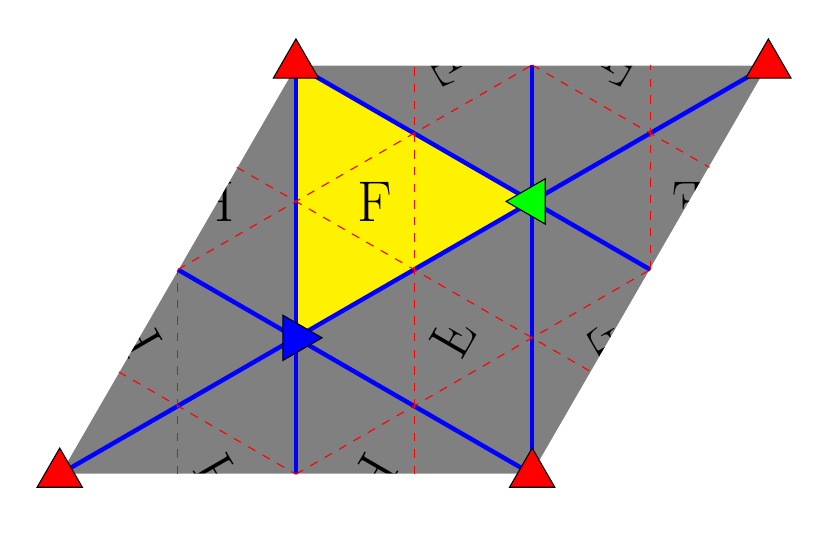
\begin{tikzpicture}
            % Define the lengths of the sides and the angle
            \def\a{3}  % length of side a
            \def\b{3}  % length of side b
            \def\angle{60}  % angle between sides a and b
            \def\s{F} % Label in center of cells

            \def\x{0.4}
            \def\y{0.4}
        
            % Calculate the coordinates of the points
            \coordinate (C00) at (0, 0);
            \coordinate (C10) at (\a, 0);
            \coordinate (C11) at ({\a + \b*cos(\angle)}, {\b * sin(\angle)});
            \coordinate (C01) at ({\b * cos(\angle)}, {\b * sin(\angle)});
            \coordinate (C02) at ({2*\b*cos(\angle)}, {2*\b * sin(\angle)});
            \coordinate (C12) at ({\a +2*\b * cos(\angle)}, {2*\b * sin(\angle)});
            \coordinate (C22) at ({2*\a + 2*\b * cos(\angle)}, {2*\b * sin(\angle)});
            \coordinate (C21) at ({2*\a + \b*cos(\angle)}, {\b * sin(\angle)});
            \coordinate (C20) at ({2*\a}, 0);
            \coordinate (A1) at ($(C00)!0.6666!(C11)$);
            \coordinate (A2) at ($(C11)!0.3333!(C22)$);
        

            % Draw the oblique unit cell
            \draw[thick,fill=gray,gray] (C00) -- (C20) -- (C22) -- (C02) -- cycle;
            \draw[thick,fill=yellow,yellow] (A1) -- (A2) -- (C02) -- cycle;
            %\draw[thick] (C10) -- (C21) -- (C12) -- (C01) -- cycle;
            

            % Draw bourdary chiral centres
            \node[rotate=240] at ($(C10)!0.3333!(C20)$) {\huge \s};
            \node[rotate=120] at ($(C00)!0.6666!(C10)$) {\reflectbox{\huge \s}};
            \node[rotate=120] at ($(C00)!0.6666!(C01)$) {\huge \s};
            \node at ($(C01)!0.3333!(C02)$) {\reflectbox{\huge \s}};
            \node[rotate=120] at ($(C02)!0.6666!(C12)$) {\reflectbox{\huge \s}};
            \node[rotate=240] at ($(C12)!0.3333!(C22)$) {\huge \s};
            \node[rotate=120] at ($(C20)!0.6666!(C21)$) {\huge \s};
            \node at ($(C21)!0.3333!(C22)$) {\reflectbox{\huge \s}};

            % Create white border
            \draw[fill=white,white] ($(C00)-(\x,\y)$) -- ($(C20)-(-\x,\y)$) -- (C20) -- (C00);
            \draw[fill=white,white] ($(C00)-(\x,-\y)$) -- ($(C02)-(\x,-\y)$) -- (C02) -- (C00);
            \draw[fill=white,white] ($(C02)+(\x,\y)$) -- ($(C22)-(\x,-\y)$) -- (C22) -- (C02);
            \draw[fill=white,white] ($(C20)+(\x,-\y)$) -- ($(C22)+(\x,\y)$) -- (C22) -- (C20);

            % Draw inner chiral centres
            \node at ($(A1)!0.5!(A2)!0.3333!(C02)$) {\huge \s};
            \node[rotate=240] at ($(A1)!0.5!(A2)!0.3333!(C20)$) {\reflectbox{\huge \s}};

        

            % Draw mirrow lines
            \draw[ultra thick,blue] (C00)--(C22);
            \draw[ultra thick,blue] (C01)--(C20);
            \draw[ultra thick,blue] (C10)--(C02);
            \draw[ultra thick,blue] (C12)--(C20);
            \draw[ultra thick,blue] (C02)--(C21);
            \draw[dashed,red] ($(C00)!0.5!(C10)$)--(C01);
            \draw[dashed,red] ($(C00)!0.5!(C01)$)--(C10);
            \draw[dashed,red] ($(C10)!0.5!(C20)$)--($(C02)!0.5!(C12)$);
            \draw[dashed,red] ($(C01)!0.5!(C02)$)--($(C20)!0.5!(C21)$);
            \draw[dashed,red] (C01)--(C12);
            \draw[dashed,red] (C10)--(C21);
            \draw[dashed,red] (C12)--($(C21)!0.5!(C22)$);
            \draw[dashed,red] (C21)--($(C12)!0.5!(C22)$);
            

            

            % Draw node reflections
            \draw (C00)  node[regular polygon, regular polygon sides=3, draw, fill=red, minimum size=0.5cm] {};
            %\draw (C10)  node[shape aspect=0.5,rotate=90,diamond,draw,fill=blue] {};
            %\draw (C11)  node[shape aspect=0.5,diamond,draw,fill=red] {};
            %\draw (C01)  node[shape aspect=0.5,rotate=90,diamond,draw,fill=blue] {};
            \draw (C02)  node[regular polygon, regular polygon sides=3, draw, fill=red, minimum size=0.5cm] {};
            %\draw (C12)  node[shape aspect=0.5,rotate=90,diamond,draw,fill=blue] {};
            \draw (C22)  node[regular polygon, regular polygon sides=3, draw, fill=red, minimum size=0.5cm] {};
            %\draw (C21)  node[shape aspect=0.5,rotate=90,diamond,draw,fill=blue] {};
            \draw (C20)  node[regular polygon, regular polygon sides=3, draw, fill=red, minimum size=0.5cm] {};

            \draw (A1)  node[rotate = 30,regular polygon, regular polygon sides=3, draw, fill=blue, minimum size=0.5cm] {};
            \draw (A2)  node[rotate=90, regular polygon, regular polygon sides=3, draw, fill=green, minimum size=0.5cm] {};

            %\draw ($(A)!0.5!(E)$) node[shape aspect=0.5,diamond,draw,fill=black] {};
            
        \end{tikzpicture}
\end{document}}
        \caption*{p3m1}
    \end{minipage}
    \hfill
    \begin{minipage}{0.10\textwidth}
        \centering
        \scalebox{0.10}{\documentclass[class=article, crop=false]{standalone}
\usepackage{tikz}
\usepackage{subcaption}
\usetikzlibrary{calc}
\usetikzlibrary {shapes.geometric}

\begin{document}
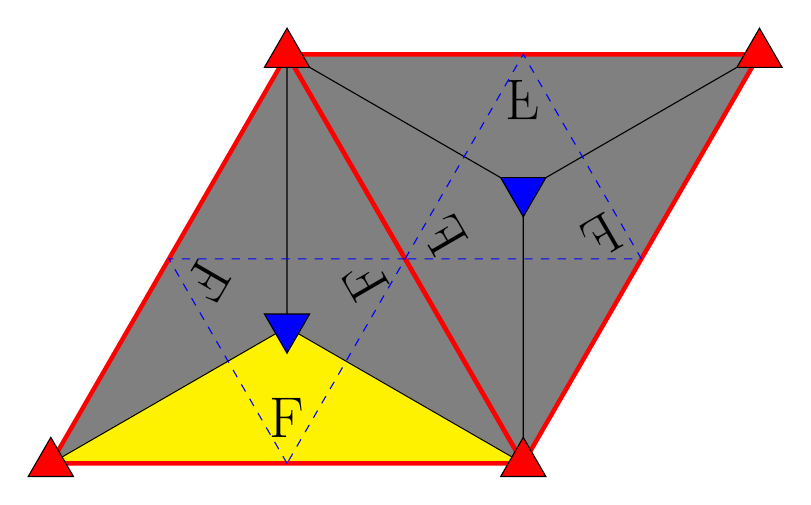
\begin{tikzpicture}
            % Define the lengths of the sides and the angle
            \def\a{3}  % length of side a
            \def\b{3}  % length of side b
            \def\angle{60}  % angle between sides a and b
            \def\s{F} % Label in center of cells

            \def\x{0.5} % Boundary 
            \def\y{0.5} % Boundary
        
            % Calculate the coordinates of the points
            \coordinate (C00) at (0, 0);
            \coordinate (C10) at (\a, 0);
            \coordinate (C11) at ({\a + \b*cos(\angle)}, {\b * sin(\angle)});
            \coordinate (C01) at ({\b * cos(\angle)}, {\b * sin(\angle)});
            \coordinate (C02) at ({2*\b*cos(\angle)}, {2*\b * sin(\angle)});
            \coordinate (C12) at ({\a +2*\b * cos(\angle)}, {2*\b * sin(\angle)});
            \coordinate (C22) at ({2*\a + 2*\b * cos(\angle)}, {2*\b * sin(\angle)});
            \coordinate (C21) at ({2*\a + \b*cos(\angle)}, {\b * sin(\angle)});
            \coordinate (C20) at ({2*\a}, 0);

            \coordinate (A1) at ($(C00)!0.6666!(C11)$);
            \coordinate (A2) at ($(C11)!0.3333!(C22)$);
        
            % Draw the oblique unit cell
            \draw[fill=gray,gray] (C00) -- (C20) -- (C22) -- (C02) -- cycle;
            \draw[fill=yellow,yellow] (C00) -- (A1) -- (C20) -- cycle;
            
            
            
            % Draw chiral center
            \node at ($(C00)!0.5!(C20)!0.3333!(A1)$) {\huge \s};
            \node[rotate=240] at ($(C00)!0.5!(C02)!0.3333!(A1)$) {\huge \s};
            \node[rotate=120] at ($(C20)!0.5!(C02)!0.3333!(A1)$) {\huge \s};
            \node[rotate=300] at ($(C20)!0.5!(C02)!0.3333!(A2)$) {\reflectbox{\huge \s}};
            \node[rotate=30] at ($(C20)!0.5!(C22)!0.3333!(A2)$) {\reflectbox{\huge \s}};
            \node[rotate=180] at ($(C02)!0.5!(C22)!0.3333!(A2)$) {\reflectbox{\huge \s}};

            % Draw mirrow lines
            \draw[ultra thick,red] (C00) -- (C02) -- (C20) -- cycle;
            \draw[ultra thick,red] (C02) -- (C22) -- (C20) -- cycle;
            \draw[thin] (C00) -- (A1) -- (C02) -- (A2) -- (C22);
            \draw[thin] (A1) -- (C20) -- (A2);
            \draw[dashed,blue] (C10) -- (C01) -- (C11) -- cycle;
            \draw[dashed,blue] (C11) -- (C12) -- (C21) -- cycle;
            

            % Draw node rotations symbols
            \draw (C00)  node[regular polygon, regular polygon sides=3, draw, fill=red, minimum size=0.5cm] {};
            \draw (C02)  node[regular polygon, regular polygon sides=3, draw, fill=red, minimum size=0.5cm] {};
            \draw (C22)  node[regular polygon, regular polygon sides=3, draw, fill=red, minimum size=0.5cm] {};
            \draw (C20)  node[regular polygon, regular polygon sides=3, draw, fill=red, minimum size=0.5cm] {};

            \draw (A1)  node[rotate = 180,regular polygon, regular polygon sides=3, draw, fill=blue, minimum size=0.5cm] {};
            \draw (A2)  node[rotate=180, regular polygon, regular polygon sides=3, draw, fill=blue, minimum size=0.5cm] {};

        \end{tikzpicture}
\end{document}}
        \caption*{p31m}
    \end{minipage}
    \caption{The 17 Wallpaper Groups}
    \label{fig:17-wallpaper-groups}
\end{figure}
\end{frame}

\begin{frame}

  \frametitle{References}
  \bibliographystyle{apalike} % We choose the "plain" reference style
  \bibliography{Sources} % Entries are in the refs.bib file
\end{frame}

\begin{frame}{p1 cell diagram}
    \begin{figure}
        \centering
        \documentclass[class=article, crop=false]{standalone}
\usepackage{tikz}
\usepackage{subcaption}
\usetikzlibrary{calc}

\begin{document}
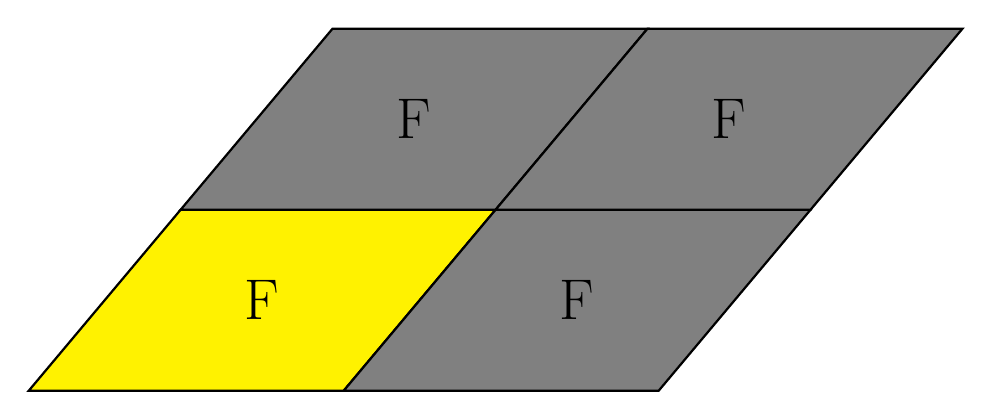
\begin{tikzpicture}
    % Define the lengths of the sides and the angle
    \def\a{4}  % length of side a
    \def\b{3}  % length of side b
    \def\angle{50}  % angle between sides a and b
    \def\s{F} % Label in center of cells

    % Calculate the coordinates of the points
    \coordinate (C00) at (0, 0);
    \coordinate (C10) at (\a, 0);
    \coordinate (C11) at ({\a + \b*cos(\angle)}, {\b * sin(\angle)});
    \coordinate (C01) at ({\b * cos(\angle)}, {\b * sin(\angle)});
    \coordinate (C02) at ({2*\b*cos(\angle)}, {2*\b * sin(\angle)});
    \coordinate (C12) at ({\a +2*\b * cos(\angle)}, {2*\b * sin(\angle)});
    \coordinate (C22) at ({2*\a + 2*\b * cos(\angle)}, {2*\b * sin(\angle)});
    \coordinate (C21) at ({2*\a + \b*cos(\angle)}, {\b * sin(\angle)});
    \coordinate (C20) at ({2*\a}, 0);

        
    % Draw the oblique unit cell
    \draw[thick,fill=yellow] (C00) -- (C10) -- (C11) -- (C01) -- cycle;
    \draw[thick,fill=gray] (C01) -- (C11) -- (C12) -- (C02) -- cycle;
    \draw[thick,fill=gray] (C10) -- (C20) -- (C21) -- (C11) -- cycle;
    \draw[thick,fill=gray] (C11) -- (C21) -- (C22) -- (C12) -- cycle;

    % Center symbols
    \node at ($(C00)!0.5!(C11)$) {\huge \s};
    \node at ($(C20)!0.5!(C11)$) {\huge \s};
    \node at ($(C02)!0.5!(C11)$) {\huge \s};
    \node at ($(C22)!0.5!(C11)$) {\huge \s};
\end{tikzpicture}
\end{document}
        \caption{p1 cell diagram.}
        \label{fig:enter-label}
    \end{figure}
\end{frame}

\begin{frame}{p2 cell diagram}
    \begin{figure}
        \centering
        \documentclass[class=article, crop=false]{standalone}
\usepackage{tikz}
\usepackage{subcaption}
\usetikzlibrary{calc}
\usetikzlibrary {shapes.geometric}

\begin{document}
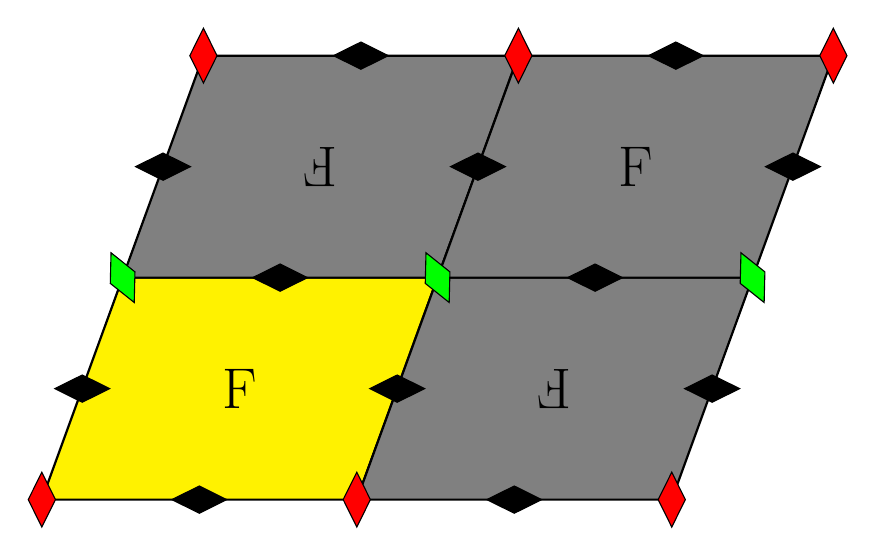
\begin{tikzpicture}
    % Define the lengths of the sides and the angle
    \def\a{4}  % length of side a
    \def\b{3}  % length of side b
    \def\angle{70}  % angle between sides a and b
    \def\s{F} % Label in center of cells

    % Calculate the coordinates of the points
    \coordinate (C00) at (0, 0);
    \coordinate (C10) at (\a, 0);
    \coordinate (C11) at ({\a + \b*cos(\angle)}, {\b * sin(\angle)});
    \coordinate (C01) at ({\b * cos(\angle)}, {\b * sin(\angle)});
    \coordinate (C02) at ({2*\b*cos(\angle)}, {2*\b * sin(\angle)});
    \coordinate (C12) at ({\a +2*\b * cos(\angle)}, {2*\b * sin(\angle)});
    \coordinate (C22) at ({2*\a + 2*\b * cos(\angle)}, {2*\b * sin(\angle)});
    \coordinate (C21) at ({2*\a + \b*cos(\angle)}, {\b * sin(\angle)});
    \coordinate (C20) at ({2*\a}, 0);
        
    % Draw the oblique unit cell
    \draw[thick,fill=yellow] (C00) -- (C10) -- (C11) -- (C01) -- cycle;
    \draw[thick,fill=gray] (C10) -- (C20) -- (C21) -- (C11) -- cycle;
    \draw[thick,fill=gray] (C01) -- (C11) -- (C12) -- (C02) -- cycle;
    \draw[thick,fill=gray] (C11) -- (C21) -- (C22) -- (C12) -- cycle;
    
    % Draw chiral center
    \node at ($(C00)!0.5!(C11)$) {\huge \s};
    \node[rotate=180] at ($(C01)!0.5!(C12)$) {\huge \s};
    \node at ($(C11)!0.5!(C22)$) {\huge \s};
    \node[rotate=180] at ($(C10)!0.5!(C21)$) {\huge \s};

    % Draw node reflections
    \draw (C00)  node[shape aspect=0.5,diamond,draw,fill=red] {};
    \draw (C10)  node[shape aspect=0.5,diamond,draw,fill=red] {};
    \draw (C20)  node[shape aspect=0.5,diamond,draw,fill=red] {};
    \draw (C01)  node[rotate = \angle-45,shape aspect=0.5,diamond,draw,fill=green] {};
    \draw (C11)  node[rotate = \angle-45,shape aspect=0.5,diamond,draw,fill=green] {};
    \draw (C21)  node[rotate = \angle-45,shape aspect=0.5,diamond,draw,fill=green] {};
    \draw (C02)  node[shape aspect=0.5,diamond,draw,fill=red] {};
    \draw (C12)  node[shape aspect=0.5,diamond,draw,fill=red] {};
    \draw (C22)  node[shape aspect=0.5,diamond,draw,fill=red] {}; 
    \draw ($(C00)!0.5!(C10)$)  node[rotate=90,shape aspect=0.5,diamond,draw,fill=black] {};
    \draw ($(C10)!0.5!(C20)$)  node[rotate=90,shape aspect=0.5,diamond,draw,fill=black] {};
    \draw ($(C00)!0.5!(C01)$)  node[rotate=90,shape aspect=0.5,diamond,draw,fill=black] {};
    \draw ($(C10)!0.5!(C11)$)  node[rotate=90,shape aspect=0.5,diamond,draw,fill=black] {};
    \draw ($(C20)!0.5!(C21)$)  node[rotate=90,shape aspect=0.5,diamond,draw,fill=black] {};
    \draw ($(C01)!0.5!(C02)$)  node[rotate=90,shape aspect=0.5,diamond,draw,fill=black] {};
    
    \draw ($(C01)!0.5!(C11)$)  node[rotate=90,shape aspect=0.5,diamond,draw,fill=black] {};
    \draw ($(C11)!0.5!(C21)$)  node[rotate=90,shape aspect=0.5,diamond,draw,fill=black] {};
    
    \draw ($(C11)!0.5!(C12)$)  node[rotate=90,shape aspect=0.5,diamond,draw,fill=black] {};
    \draw ($(C21)!0.5!(C22)$)  node[rotate=90,shape aspect=0.5,diamond,draw,fill=black] {};
    \draw ($(C02)!0.5!(C12)$)  node[rotate=90,shape aspect=0.5,diamond,draw,fill=black] {};
    \draw ($(C12)!0.5!(C22)$)  node[rotate=90,shape aspect=0.5,diamond,draw,fill=black] {};
\end{tikzpicture}
\end{document}
        \caption{p2 cell diagram.}
        \label{fig:enter-label}
    \end{figure}
\end{frame}

\begin{frame}{pm cell diagram}
    \begin{figure}
        \centering
        \documentclass[class=article, crop=false]{standalone}
\usepackage{tikz}
\usepackage{subcaption}
\usetikzlibrary{calc}
\usetikzlibrary {shapes.geometric}

\begin{document}
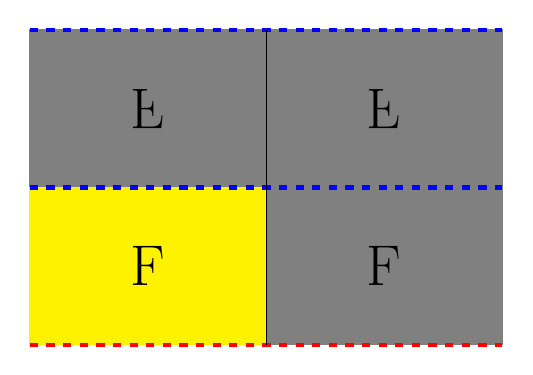
\begin{tikzpicture}
            % Define the lengths of the sides and the angle
            \def\a{3}  % length of side a
            \def\b{2}  % length of side b
            \def\angle{90}  % angle between sides a and b
            \def\s{F} % Label in center of cells

            \def\x{0.5} % Boundary 
            \def\y{0.5} % Boundary
        
            % Calculate the coordinates of the points
            \coordinate (C00) at (0, 0);
            \coordinate (C10) at (\a, 0);
            \coordinate (C11) at ({\a + \b*cos(\angle)}, {\b * sin(\angle)});
            \coordinate (C01) at ({\b * cos(\angle)}, {\b * sin(\angle)});
            \coordinate (C02) at ({2*\b*cos(\angle)}, {2*\b * sin(\angle)});
            \coordinate (C12) at ({\a +2*\b * cos(\angle)}, {2*\b * sin(\angle)});
            \coordinate (C22) at ({2*\a + 2*\b * cos(\angle)}, {2*\b * sin(\angle)});
            \coordinate (C21) at ({2*\a + \b*cos(\angle)}, {\b * sin(\angle)});
            \coordinate (C20) at ({2*\a}, 0);

            \coordinate (A1) at ($(C00)!0.6666!(C11)$);
            \coordinate (A2) at ($(C11)!0.3333!(C22)$);
        
            % Draw the oblique unit cell
            \draw[fill=gray,gray] (C00) -- (C20) -- (C22) -- (C02) -- cycle;
            \draw[fill=yellow,yellow] (C00) -- (C10) -- (C11) -- (C01) -- cycle;


            % Draw mirror lines
            \draw[ultra thick,blue,dashed] (C01) -- (C21);
            \draw[ultra thick,red,dashed] (C00) -- (C20);
            \draw[ultra thick,blue,dashed] (C02) -- (C22);
            \draw[] (C10) -- (C12);
            
           
            
            % Draw chiral center
            \node at ($(C00)!0.5!(C11)$) {\huge F};
            \node[rotate=180] at ($(C01)!0.5!(C12)$) {\reflectbox{\huge F}};
            \node at ($(C10)!0.5!(C21)$) {\huge F};
            \node[rotate=180] at ($(C11)!0.5!(C22)$) {\reflectbox{\huge F}};

            
        \end{tikzpicture}
\end{document}
        \caption{pm cell diagram.}
        \label{fig:enter-label}
    \end{figure}
\end{frame}

\begin{frame}{pg cell diagram}
    \begin{figure}
        \centering
        \documentclass[class=article, crop=false]{standalone}
\usepackage{tikz}
\usepackage{subcaption}
\usetikzlibrary{calc}
\usetikzlibrary {shapes.geometric}

\begin{document}
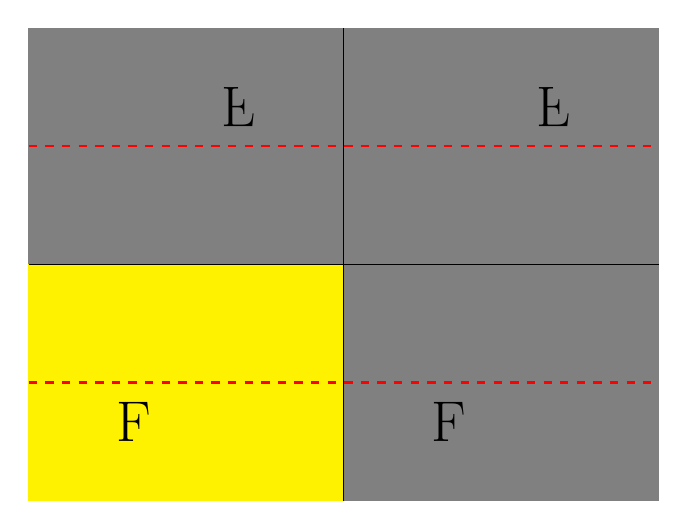
\begin{tikzpicture}
            % Define the lengths of the sides and the angle
            \def\a{4}  % length of side a
            \def\b{3}  % length of side b
            \def\angle{90}  % angle between sides a and b
            \def\s{F} % Label in center of cells


        
            % Calculate the coordinates of the points
            \coordinate (C00) at (0, 0);
            \coordinate (C10) at (\a, 0);
            \coordinate (C11) at ({\a + \b*cos(\angle)}, {\b * sin(\angle)});
            \coordinate (C01) at ({\b * cos(\angle)}, {\b * sin(\angle)});
            \coordinate (C02) at ({2*\b*cos(\angle)}, {2*\b * sin(\angle)});
            \coordinate (C12) at ({\a +2*\b * cos(\angle)}, {2*\b * sin(\angle)});
            \coordinate (C22) at ({2*\a + 2*\b * cos(\angle)}, {2*\b * sin(\angle)});
            \coordinate (C21) at ({2*\a + \b*cos(\angle)}, {\b * sin(\angle)});
            \coordinate (C20) at ({2*\a}, 0);

            \coordinate (A1) at ($(C00)!0.6666!(C11)$);
            \coordinate (A2) at ($(C11)!0.3333!(C22)$);
        
            % Draw the oblique unit cell
            \draw[fill=gray,gray] (C00) -- (C20) -- (C22) -- (C02) -- cycle;
            \draw[fill=yellow,yellow] (C00) -- (C01) -- (C11) -- (C10) -- cycle;
            \draw[] (C01) -- (C11) -- (C12);
            \draw[] (C10) -- (C11) -- (C21);
            
            % Draw chiral center
            \node at ($(C00)!0.3333!(C11)$) {\huge \s};
            \node at ($(C10)!0.3333!(C21)$) {\huge \s};
            \node[rotate=180] at ($(C11)!0.6666!(C22)$) {\reflectbox{\huge \s}};
            \node[rotate=180] at ($(C01)!0.6666!(C12)$) {\reflectbox{\huge \s}};

            % Draw mirror lines
            \draw[thick,dashed,red] ($(C00)!0.5!(C01)$) -- ($(C20)!0.5!(C21)$);
            \draw[thick,dashed,red] ($(C01)!0.5!(C02)$) -- ($(C21)!0.5!(C22)$);

            
        \end{tikzpicture}
\end{document}
        \caption{pg cell diagram.}
        \label{fig:enter-label}
    \end{figure}
\end{frame}

\begin{frame}{cm cell diagram}
    \begin{figure}
        \centering
        \documentclass[class=article, crop=false]{standalone}
\usepackage{tikz}
\usepackage{subcaption}
\usetikzlibrary{calc}
\usetikzlibrary {shapes.geometric}

\begin{document}
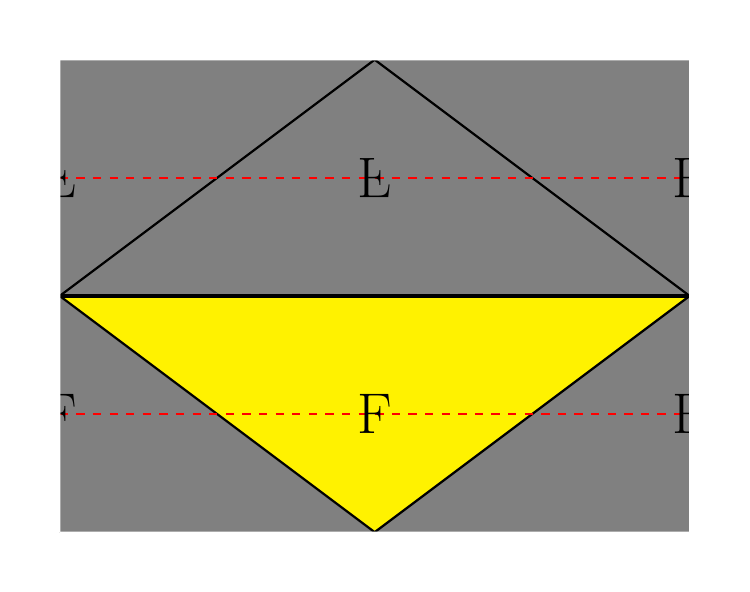
\begin{tikzpicture}
    % Define the lengths of the sides and the angle
    \def\a{4}  % length of side a
    \def\b{3}  % length of side b
    \def\angle{90}  % angle between sides a and b
    \def\s{F} % Label in center of cells

    \def\x{0.4}
    \def\y{0.4}

    % Calculate the coordinates of the points
    \coordinate (C00) at (0, 0);
    \coordinate (C10) at (\a, 0);
    \coordinate (C11) at ({\a + \b*cos(\angle)}, {\b * sin(\angle)});
    \coordinate (C01) at ({\b * cos(\angle)}, {\b * sin(\angle)});
    \coordinate (C02) at ({2*\b*cos(\angle)}, {2*\b * sin(\angle)});
    \coordinate (C12) at ({\a +2*\b * cos(\angle)}, {2*\b * sin(\angle)});
    \coordinate (C22) at ({2*\a + 2*\b * cos(\angle)}, {2*\b * sin(\angle)});
    \coordinate (C21) at ({2*\a + \b*cos(\angle)}, {\b * sin(\angle)});
    \coordinate (C20) at ({2*\a}, 0);

        
    % Draw the oblique unit cell
    \draw[fill=gray,gray] (C00) -- (C20) -- (C22) -- (C02) -- cycle;
    \draw[fill=yellow,yellow] (C10) -- (C21) -- (C01) -- cycle;

    % Draw mirror lines
    \draw[ultra thick] (C01) -- (C21);
    \draw[thick] (C10) -- (C21) -- (C12) -- (C01) -- cycle;
    \draw[thick,dashed,red] ($(C00)!0.5!(C01)$) -- ($(C20)!0.5!(C21)$);
    \draw[thick,dashed,red] ($(C01)!0.5!(C02)$) -- ($(C21)!0.5!(C22)$);

    

    % Draw boundary centre symbols
    \node at ($(C00)!0.5!(C01)$) {\huge \s};
    \node[rotate=180] at ($(C01)!0.5!(C02)$) {\reflectbox{\huge \s}};
    \node at ($(C20)!0.5!(C21)$) {\huge \s};
    \node[rotate=180] at ($(C21)!0.5!(C22)$) {\reflectbox{\huge \s}};

    % Create white border
    \draw[fill=white,white] ($(C00)-(\x,\y)$) -- ($(C20)-(-\x,\y)$) -- (C20) -- (C00);
    \draw[fill=white,white] ($(C00)-(\x,-\y)$) -- ($(C02)-(\x,-\y)$) -- (C02) -- (C00);
    \draw[fill=white,white] ($(C02)+(\x,\y)$) -- ($(C22)-(\x,-\y)$) -- (C22) -- (C02);
    \draw[fill=white,white] ($(C20)+(\x,-\y)$) -- ($(C22)+(\x,\y)$) -- (C22) -- (C20);
    
    % Center symbols
    \node at ($(C10)!0.5!(C11)$) {\huge \s};
    \node[rotate=180] at ($(C11)!0.5!(C12)$) {\reflectbox{\huge \s}};
    
\end{tikzpicture}
\end{document}
        \caption{cm cell diagram.}
        \label{fig:enter-label}
    \end{figure}
\end{frame}

\begin{frame}{cmm cell diagram}
    \begin{figure}
        \centering
        \documentclass[class=article, crop=false]{standalone}
\usepackage{tikz}
\usepackage{subcaption}
\usetikzlibrary{calc}
\usetikzlibrary {shapes.geometric}

\begin{document}
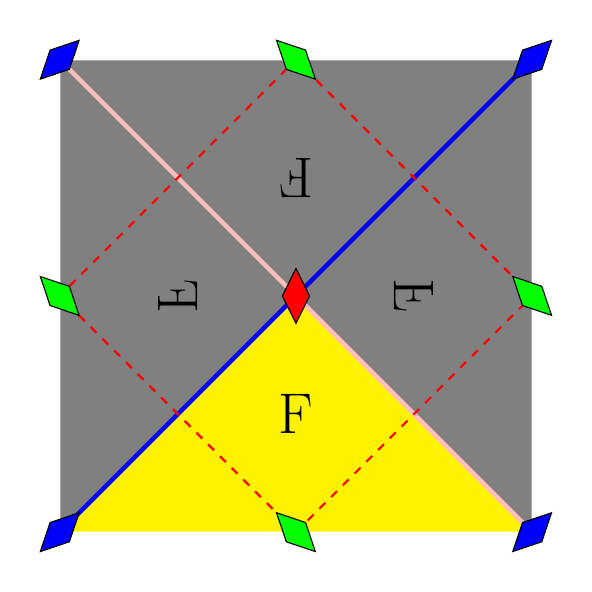
\begin{tikzpicture}
    % Define the lengths of the sides and the angle
    \def\a{3}  % length of side a
    \def\b{3}  % length of side b
    \def\angle{90}  % angle between sides a and b
    \def\s{F} % Label in center of cells

    \def\x{0.4}
    \def\y{0.4}

    % Calculate the coordinates of the points
    \coordinate (C00) at (0, 0);
    \coordinate (C10) at (\a, 0);
    \coordinate (C11) at ({\a + \b*cos(\angle)}, {\b * sin(\angle)});
    \coordinate (C01) at ({\b * cos(\angle)}, {\b * sin(\angle)});
    \coordinate (C02) at ({2*\b*cos(\angle)}, {2*\b * sin(\angle)});
    \coordinate (C12) at ({\a +2*\b * cos(\angle)}, {2*\b * sin(\angle)});
    \coordinate (C22) at ({2*\a + 2*\b * cos(\angle)}, {2*\b * sin(\angle)});
    \coordinate (C21) at ({2*\a + \b*cos(\angle)}, {\b * sin(\angle)});
    \coordinate (C20) at ({2*\a}, 0);

        
    % Draw the oblique unit cell
    \draw[fill=gray,gray] (C00) -- (C20) -- (C22) -- (C02) -- cycle;
    \draw[fill=yellow,yellow] (C00) -- (C11) -- (C20) -- cycle;

    % Draw mirror lines
    \draw[ultra thick,blue] (C00) -- (C22);
    \draw[ultra thick,pink] (C20) -- (C02);
    \draw[thick,dashed,red] (C10) -- (C21) -- (C12) -- (C01) -- cycle;
    
    

    % Draw boundary centre symbols
    %\node[rotate=180] at ($(C00)!0.5!(C01)$) {\huge \s};
    %\node[rotate=0] at ($(C01)!0.5!(C02)$) {\reflectbox{\huge \s}};
    %\node at ($(C20)!0.5!(C21)$) {\huge \s};
    %\node[rotate=180] at ($(C21)!0.5!(C22)$) {\reflectbox{\huge \s}};

    % Create white border
    \draw[fill=white,white] ($(C00)-(\x,\y)$) -- ($(C20)-(-\x,\y)$) -- (C20) -- (C00);
    \draw[fill=white,white] ($(C00)-(\x,-\y)$) -- ($(C02)-(\x,-\y)$) -- (C02) -- (C00);
    \draw[fill=white,white] ($(C02)+(\x,\y)$) -- ($(C22)-(\x,-\y)$) -- (C22) -- (C02);
    \draw[fill=white,white] ($(C20)+(\x,-\y)$) -- ($(C22)+(\x,\y)$) -- (C22) -- (C20);
    
    % Center symbols
    \node at ($(C10)!0.5!(C11)$) {\huge \s};
    \node[rotate=270] at ($(C01)!0.5!(C11)$) {\reflectbox{\huge \s}};
    \node[rotate=180] at ($(C12)!0.5!(C11)$) {\huge \s};
    \node[rotate=90] at ($(C21)!0.5!(C11)$) {\reflectbox{\huge \s}};

    % Draw node rotations
    \draw (C11)  node[rotate = 0,shape aspect=0.5,diamond,draw,fill=red] {};
    \draw (C10)  node[rotate = 45,shape aspect=0.5,diamond,draw,fill=green] {};
    \draw (C01)  node[rotate = 45,shape aspect=0.5,diamond,draw,fill=green] {};
    \draw (C21)  node[rotate = 45,shape aspect=0.5,diamond,draw,fill=green] {};
    \draw (C12)  node[rotate = 45,shape aspect=0.5,diamond,draw,fill=green] {};
    \draw (C00)  node[rotate = 135,shape aspect=0.5,diamond,draw,fill=blue] {};
    \draw (C20)  node[rotate = 135,shape aspect=0.5,diamond,draw,fill=blue] {};
    \draw (C02)  node[rotate = 135,shape aspect=0.5,diamond,draw,fill=blue] {};
    \draw (C22)  node[rotate = 135,shape aspect=0.5,diamond,draw,fill=blue] {};
    
\end{tikzpicture}
\end{document}
        \caption{cmm cell diagram.}
        \label{fig:enter-label}
    \end{figure}
\end{frame}
\begin{frame}{pmm cell diagram}
    \begin{figure}
        \centering
        \documentclass[class=article, crop=false]{standalone}
\usepackage{tikz}
\usepackage{subcaption}
\usetikzlibrary{calc}
\usetikzlibrary {shapes.geometric}

\begin{document}
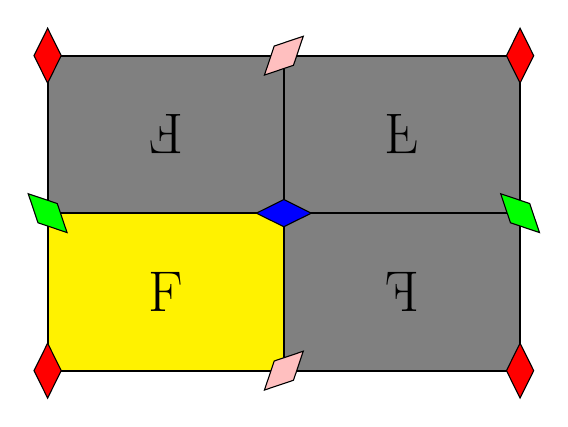
\begin{tikzpicture}
            % Define the lengths of the sides and the angle
            \def\a{3}  % length of side a
            \def\b{2}  % length of side b
            \def\angle{90}  % angle between sides a and b
            \def\s{F}

        
            % Calculate the coordinates of the points
            \coordinate (C00) at (0, 0);
            \coordinate (C10) at (\a, 0);
            \coordinate (C11) at ({\a + \b*cos(\angle)}, {\b * sin(\angle)});
            \coordinate (C01) at ({\b * cos(\angle)}, {\b * sin(\angle)});
            \coordinate (C02) at ({2*\b*cos(\angle)}, {2*\b * sin(\angle)});
            \coordinate (C12) at ({\a +2*\b * cos(\angle)}, {2*\b * sin(\angle)});
            \coordinate (C22) at ({2*\a + 2*\b * cos(\angle)}, {2*\b * sin(\angle)});
            \coordinate (C21) at ({2*\a + \b*cos(\angle)}, {\b * sin(\angle)});
            \coordinate (C20) at ({2*\a}, 0);
        
            % Draw the oblique unit cell
            \draw[thick,fill=yellow] (C00) -- (C01) -- (C11) -- (C10) -- cycle;
            \draw[thick,fill=gray] (C01) -- (C11) -- (C12) -- (C02) -- cycle;
            
            \draw[thick,fill=gray] (C11) -- (C12) -- (C22) -- (C21) -- cycle;
            \draw[thick,fill=gray] (C10) -- (C20) -- (C21) -- (C11) -- cycle;
            
            % Draw chiral center
            \node at ($(C00)!0.5!(C11)$) {\huge \s};
            \node[rotate=180] at ($(C01)!0.5!(C12)$) {\huge \s};
            \node at ($(C10)!0.5!(C21)$) {\reflectbox{\huge \s}};
            \node[rotate=180] at ($(C11)!0.5!(C22)$) {\reflectbox{\huge \s}};

            % Draw node reflections
            \draw (C00)  node[shape aspect=0.5,diamond,draw,fill=red] {};
            \draw (C10)  node[shape aspect=0.5,rotate=-45,diamond,draw,fill=pink] {};
            \draw (C11)  node[rotate = \angle,shape aspect=0.5,diamond,draw,fill=blue] {};
            \draw (C01)  node[shape aspect=0.5,rotate=45,diamond,draw,fill=green] {};
            \draw (C02)  node[shape aspect=0.5,diamond,draw,fill=red] {};
            \draw (C12)  node[shape aspect=0.5,rotate=-45,diamond,draw,fill=pink] {};
            \draw (C22)  node[shape aspect=0.5,diamond,draw,fill=red] {};
            \draw (C21)  node[shape aspect=0.5,rotate=45,diamond,draw,fill=green] {};
            \draw (C20)  node[shape aspect=0.5,diamond,draw,fill=red] {};

            %\draw ($(A)!0.5!(E)$) node[shape aspect=0.5,diamond,draw,fill=black] {};
            
        \end{tikzpicture}
\end{document}
        \caption{pmm cell diagram.}
        \label{fig:enter-label}
    \end{figure}
\end{frame}
\begin{frame}{pmg cell diagram}
    \begin{figure}
        \centering
        \documentclass[class=article, crop=false]{standalone}
\usepackage{tikz}
\usepackage{subcaption}
\usetikzlibrary{calc}
\usetikzlibrary {shapes.geometric}

\begin{document}
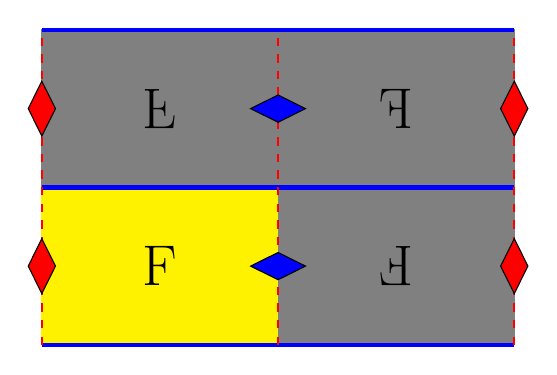
\begin{tikzpicture}
            % Define the lengths of the sides and the angle
            \def\a{3}  % length of side a
            \def\b{2}  % length of side b
            \def\angle{90}  % angle between sides a and b
            \def\s{F}
        
            % Calculate the coordinates of the points
            \coordinate (C00) at (0, 0);
            \coordinate (C10) at (\a, 0);
            \coordinate (C11) at ({\a + \b*cos(\angle)}, {\b * sin(\angle)});
            \coordinate (C01) at ({\b * cos(\angle)}, {\b * sin(\angle)});
            \coordinate (C02) at ({2*\b*cos(\angle)}, {2*\b * sin(\angle)});
            \coordinate (C12) at ({\a +2*\b * cos(\angle)}, {2*\b * sin(\angle)});
            \coordinate (C22) at ({2*\a + 2*\b * cos(\angle)}, {2*\b * sin(\angle)});
            \coordinate (C21) at ({2*\a + \b*cos(\angle)}, {\b * sin(\angle)});
            \coordinate (C20) at ({2*\a}, 0);
        
            % Draw the oblique unit cell
            \draw[fill=yellow,yellow] (C00) -- (C01) -- (C11) -- (C10) -- cycle;
            \draw[fill=gray,gray] (C01) -- (C11) -- (C12) -- (C02) -- cycle;
            
            \draw[fill=gray,gray] (C11) -- (C12) -- (C22) -- (C21) -- cycle;
            \draw[fill=gray,gray] (C10) -- (C20) -- (C21) -- (C11) -- cycle;

            % Draw mirror lines
            \draw[ultra thick,blue] (C00) -- (C20);
            \draw[ultra thick,blue] (C01) -- (C21);
            \draw[ultra thick,blue] (C02) -- (C22);
            \draw[thick,dashed,red] (C00) -- (C02);
            \draw[thick,dashed,red] (C10) -- (C12);
            \draw[thick,dashed,red] (C20) -- (C22);
            
            % Draw chiral center
            \node at ($(C00)!0.5!(C11)$) {\huge \s};
            \node[rotate=180] at ($(C01)!0.5!(C12)$) {\reflectbox{\huge \s}};
            \node[rotate=180] at ($(C10)!0.5!(C21)$) {\huge \s};
            \node[rotate=0] at ($(C11)!0.5!(C22)$) {\reflectbox{\huge \s}};

            % Draw node rotations
            \draw ($(C00)!0.5!(C01)$)  node[shape aspect=0.5,diamond,draw,fill=red] {};
            \draw ($(C01)!0.5!(C02)$)  node[shape aspect=0.5,diamond,draw,fill=red] {};
            \draw ($(C10)!0.5!(C11)$)  node[rotate = 90,shape aspect=0.5,diamond,draw,fill=blue] {};
            \draw ($(C11)!0.5!(C12)$)  node[shape aspect=0.5,rotate=90,diamond,draw,fill=blue] {};
            \draw ($(C20)!0.5!(C21)$)  node[shape aspect=0.5,diamond,draw,fill=red] {};
            \draw ($(C21)!0.5!(C22)$)  node[shape aspect=0.5,diamond,draw,fill=red] {};
            
        \end{tikzpicture}
\end{document}
        \caption{pmg cell diagram.}
        \label{fig:enter-label}
    \end{figure}
\end{frame}
\begin{frame}{pgg cell diagram}
    \begin{figure}
        \centering
        \documentclass[class=article, crop=false]{standalone}
\usepackage{tikz}
\usepackage{subcaption}
\usetikzlibrary{calc}
\usetikzlibrary {shapes.geometric}

\begin{document}
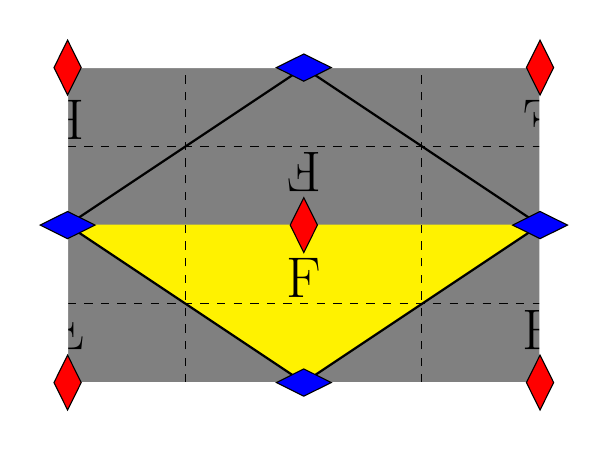
\begin{tikzpicture}
            % Define the lengths of the sides and the angle
            \def\a{3}  % length of side a
            \def\b{2}  % length of side b
            \def\angle{90}  % angle between sides a and b
            \def\s{F}

            \def\x{0.5} % Boundary 
            \def\y{0.5} % Boundary
        
            % Calculate the coordinates of the points
            \coordinate (C00) at (0, 0);
            \coordinate (C10) at (\a, 0);
            \coordinate (C11) at ({\a + \b*cos(\angle)}, {\b * sin(\angle)});
            \coordinate (C01) at ({\b * cos(\angle)}, {\b * sin(\angle)});
            \coordinate (C02) at ({2*\b*cos(\angle)}, {2*\b * sin(\angle)});
            \coordinate (C12) at ({\a +2*\b * cos(\angle)}, {2*\b * sin(\angle)});
            \coordinate (C22) at ({2*\a + 2*\b * cos(\angle)}, {2*\b * sin(\angle)});
            \coordinate (C21) at ({2*\a + \b*cos(\angle)}, {\b * sin(\angle)});
            \coordinate (C20) at ({2*\a}, 0);
        
            % Draw the oblique unit cell
            \draw[fill=gray,gray] (C00) -- (C20) -- (C22) -- (C02) -- cycle;
            \draw[fill=yellow,yellow] (C01) -- (C10) -- (C21) -- cycle;
            \draw[thick] (C10) -- (C21) -- (C12) -- (C01) -- cycle;
            
            % Draw mirrow lines
            \draw[dashed] ($(C00)!0.5!(C01)$) -- ($(C20)!0.5!(C21)$);
            \draw[dashed] ($(C01)!0.5!(C02)$) -- ($(C21)!0.5!(C22)$);
            \draw[dashed] ($(C00)!0.5!(C10)$) -- ($(C02)!0.5!(C12)$);
            \draw[dashed] ($(C10)!0.5!(C20)$) -- ($(C12)!0.5!(C22)$);


            % Draw inner centres
            \node at ($(C01)!0.6666!(C02)$) {\reflectbox{\huge \s}};
            \node[rotate=180] at ($(C00)!0.3333!(C01)$) {\reflectbox{\huge \s}};
            \node at ($(C21)!0.6666!(C22)$) {\reflectbox{\huge \s}};
            \node[rotate=180] at ($(C20)!0.3333!(C21)$) {\reflectbox{\huge \s}};

            % Create white border
            \draw[fill=white,white] ($(C00)-(\x,\y)$) -- ($(C20)-(-\x,\y)$) -- (C20) -- (C00);
            \draw[fill=white,white] ($(C00)-(\x,-\y)$) -- ($(C02)-(\x,-\y)$) -- (C02) -- (C00);
            \draw[fill=white,white] ($(C02)+(\x,\y)$) -- ($(C22)-(\x,-\y)$) -- (C22) -- (C02);
            \draw[fill=white,white] ($(C20)+(\x,-\y)$) -- ($(C22)+(\x,\y)$) -- (C22) -- (C20);
            
            % Draw chiral center
            \node at ($(C10)!0.6666!(C11)$) {\huge \s};
            \node[rotate=180] at ($(C11)!0.3333!(C12)$) {\huge \s};
            

            % Draw node reflections
            \draw (C00)  node[shape aspect=0.5,diamond,draw,fill=red] {};
            \draw (C10)  node[shape aspect=0.5,rotate=90,diamond,draw,fill=blue] {};
            \draw (C11)  node[shape aspect=0.5,diamond,draw,fill=red] {};
            \draw (C01)  node[shape aspect=0.5,rotate=90,diamond,draw,fill=blue] {};
            \draw (C02)  node[shape aspect=0.5,diamond,draw,fill=red] {};
            \draw (C12)  node[shape aspect=0.5,rotate=90,diamond,draw,fill=blue] {};
            \draw (C22)  node[shape aspect=0.5,diamond,draw,fill=red] {};
            \draw (C21)  node[shape aspect=0.5,rotate=90,diamond,draw,fill=blue] {};
            \draw (C20)  node[shape aspect=0.5,diamond,draw,fill=red] {};
        \end{tikzpicture}
\end{document}
        \caption{pgg cell diagram.}
        \label{fig:enter-label}
    \end{figure}
\end{frame}
\begin{frame}{cmm cell diagram}
    \begin{figure}
        \centering
        \documentclass[class=article, crop=false]{standalone}
\usepackage{tikz}
\usepackage{subcaption}
\usetikzlibrary{calc}
\usetikzlibrary {shapes.geometric}

\begin{document}
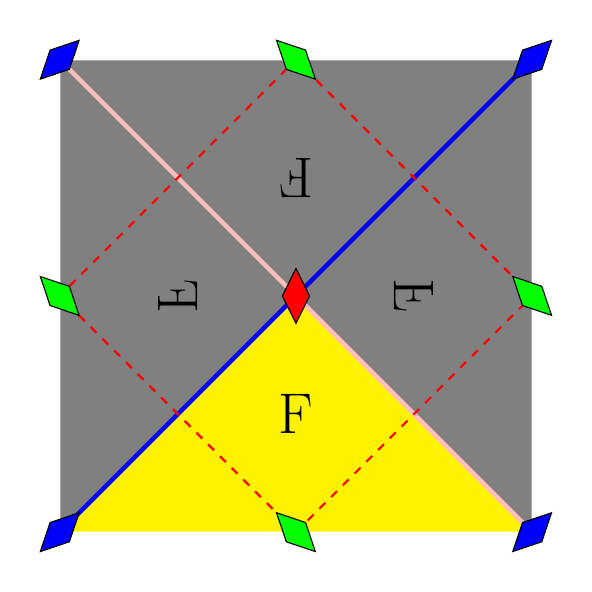
\begin{tikzpicture}
    % Define the lengths of the sides and the angle
    \def\a{3}  % length of side a
    \def\b{3}  % length of side b
    \def\angle{90}  % angle between sides a and b
    \def\s{F} % Label in center of cells

    \def\x{0.4}
    \def\y{0.4}

    % Calculate the coordinates of the points
    \coordinate (C00) at (0, 0);
    \coordinate (C10) at (\a, 0);
    \coordinate (C11) at ({\a + \b*cos(\angle)}, {\b * sin(\angle)});
    \coordinate (C01) at ({\b * cos(\angle)}, {\b * sin(\angle)});
    \coordinate (C02) at ({2*\b*cos(\angle)}, {2*\b * sin(\angle)});
    \coordinate (C12) at ({\a +2*\b * cos(\angle)}, {2*\b * sin(\angle)});
    \coordinate (C22) at ({2*\a + 2*\b * cos(\angle)}, {2*\b * sin(\angle)});
    \coordinate (C21) at ({2*\a + \b*cos(\angle)}, {\b * sin(\angle)});
    \coordinate (C20) at ({2*\a}, 0);

        
    % Draw the oblique unit cell
    \draw[fill=gray,gray] (C00) -- (C20) -- (C22) -- (C02) -- cycle;
    \draw[fill=yellow,yellow] (C00) -- (C11) -- (C20) -- cycle;

    % Draw mirror lines
    \draw[ultra thick,blue] (C00) -- (C22);
    \draw[ultra thick,pink] (C20) -- (C02);
    \draw[thick,dashed,red] (C10) -- (C21) -- (C12) -- (C01) -- cycle;
    
    

    % Draw boundary centre symbols
    %\node[rotate=180] at ($(C00)!0.5!(C01)$) {\huge \s};
    %\node[rotate=0] at ($(C01)!0.5!(C02)$) {\reflectbox{\huge \s}};
    %\node at ($(C20)!0.5!(C21)$) {\huge \s};
    %\node[rotate=180] at ($(C21)!0.5!(C22)$) {\reflectbox{\huge \s}};

    % Create white border
    \draw[fill=white,white] ($(C00)-(\x,\y)$) -- ($(C20)-(-\x,\y)$) -- (C20) -- (C00);
    \draw[fill=white,white] ($(C00)-(\x,-\y)$) -- ($(C02)-(\x,-\y)$) -- (C02) -- (C00);
    \draw[fill=white,white] ($(C02)+(\x,\y)$) -- ($(C22)-(\x,-\y)$) -- (C22) -- (C02);
    \draw[fill=white,white] ($(C20)+(\x,-\y)$) -- ($(C22)+(\x,\y)$) -- (C22) -- (C20);
    
    % Center symbols
    \node at ($(C10)!0.5!(C11)$) {\huge \s};
    \node[rotate=270] at ($(C01)!0.5!(C11)$) {\reflectbox{\huge \s}};
    \node[rotate=180] at ($(C12)!0.5!(C11)$) {\huge \s};
    \node[rotate=90] at ($(C21)!0.5!(C11)$) {\reflectbox{\huge \s}};

    % Draw node rotations
    \draw (C11)  node[rotate = 0,shape aspect=0.5,diamond,draw,fill=red] {};
    \draw (C10)  node[rotate = 45,shape aspect=0.5,diamond,draw,fill=green] {};
    \draw (C01)  node[rotate = 45,shape aspect=0.5,diamond,draw,fill=green] {};
    \draw (C21)  node[rotate = 45,shape aspect=0.5,diamond,draw,fill=green] {};
    \draw (C12)  node[rotate = 45,shape aspect=0.5,diamond,draw,fill=green] {};
    \draw (C00)  node[rotate = 135,shape aspect=0.5,diamond,draw,fill=blue] {};
    \draw (C20)  node[rotate = 135,shape aspect=0.5,diamond,draw,fill=blue] {};
    \draw (C02)  node[rotate = 135,shape aspect=0.5,diamond,draw,fill=blue] {};
    \draw (C22)  node[rotate = 135,shape aspect=0.5,diamond,draw,fill=blue] {};
    
\end{tikzpicture}
\end{document}
        \caption{cmm cell diagram.}
        \label{fig:enter-label}
    \end{figure}
\end{frame}
\begin{frame}{p4 cell diagram}
    \begin{figure}
        \centering
        \documentclass[class=article, crop=false]{standalone}
\usepackage{tikz}
\usepackage{subcaption}
\usetikzlibrary{calc}
\usetikzlibrary {shapes.geometric}

\begin{document}
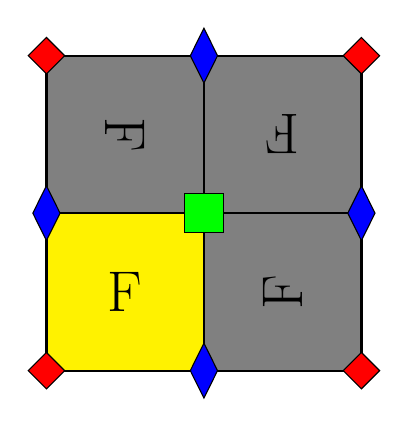
\begin{tikzpicture}
            % Define the lengths of the sides and the angle
            \def\a{2}  % length of side a
            \def\b{2}  % length of side b
            \def\angle{90}  % angle between sides a and b
            \def\s{F}
        
            % Calculate the coordinates of the points
            \coordinate (C00) at (0, 0);
            \coordinate (C10) at (\a, 0);
            \coordinate (C11) at ({\a + \b*cos(\angle)}, {\b * sin(\angle)});
            \coordinate (C01) at ({\b * cos(\angle)}, {\b * sin(\angle)});
            \coordinate (C02) at ({2*\b*cos(\angle)}, {2*\b * sin(\angle)});
            \coordinate (C12) at ({\a +2*\b * cos(\angle)}, {2*\b * sin(\angle)});
            \coordinate (C22) at ({2*\a + 2*\b * cos(\angle)}, {2*\b * sin(\angle)});
            \coordinate (C21) at ({2*\a + \b*cos(\angle)}, {\b * sin(\angle)});
            \coordinate (C20) at ({2*\a}, 0);
        
            % Draw the oblique unit cell
            \draw[thick,fill=yellow] (C00) -- (C01) -- (C11) -- (C10) -- cycle;
            \draw[thick,fill=gray] (C01) -- (C11) -- (C12) -- (C02) -- cycle;
            
            \draw[thick,fill=gray] (C11) -- (C12) -- (C22) -- (C21) -- cycle;
            \draw[thick,fill=gray] (C10) -- (C20) -- (C21) -- (C11) -- cycle;
            
            % Draw chiral center
            \node at ($(C00)!0.5!(C11)$) {\huge \s};
            \node[rotate=-90] at ($(C01)!0.5!(C12)$) {\huge \s};
            \node[rotate=90] at ($(C10)!0.5!(C21)$) {\huge \s};
            \node[rotate=180] at ($(C11)!0.5!(C22)$) {\huge \s};

            % Draw node reflections and rotations
            \draw (C00)  node[shape aspect=1,diamond,draw,fill=red] {};
            \draw (C10)  node[shape aspect=0.5,diamond,draw,fill=blue] {};
            \draw (C11)  node[minimum size=0.5cm,draw,fill=green] {};
            \draw (C01)  node[shape aspect=0.5,diamond,draw,fill=blue] {};
            \draw (C02)  node[shape aspect=1,diamond,draw,fill=red] {};
            \draw (C12)  node[shape aspect=0.5,diamond,draw,fill=blue] {};
            \draw (C22)  node[shape aspect=1,diamond,draw,fill=red] {};
            \draw (C21)  node[shape aspect=0.5,diamond,draw,fill=blue] {};
            \draw (C20)  node[shape aspect=1,diamond,draw,fill=red] {};

            %\draw ($(A)!0.5!(E)$) node[shape aspect=0.5,diamond,draw,fill=black] {};
            
        \end{tikzpicture}
\end{document}
        \caption{p4 cell diagram.}
        \label{fig:enter-label}
    \end{figure}
\end{frame}
\begin{frame}{p4m cell diagram}
    \begin{figure}
        \centering
        \documentclass[class=article, crop=false]{standalone}
\usepackage{tikz}
\usepackage{subcaption}
\usetikzlibrary{calc}
\usetikzlibrary {shapes.geometric}

\begin{document}
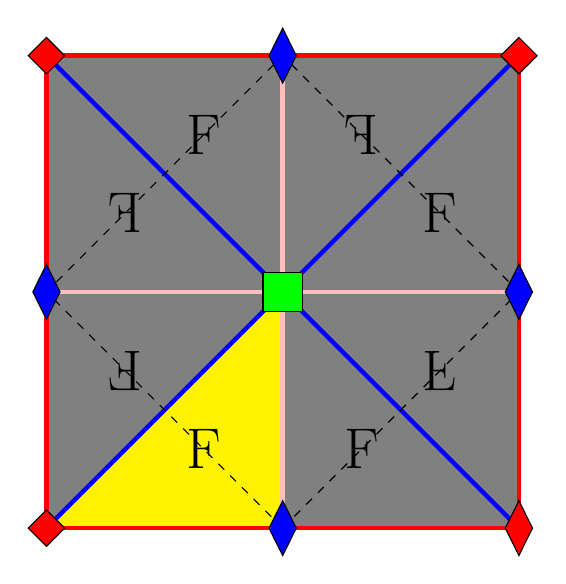
\begin{tikzpicture}
            % Define the lengths of the sides and the angle
            \def\a{3}  % length of side a
            \def\b{3}  % length of side b
            \def\angle{90}  % angle between sides a and b
            \def\s{F}
        
            % Calculate the coordinates of the points
            \coordinate (C00) at (0, 0);
            \coordinate (C10) at (\a, 0);
            \coordinate (C11) at ({\a + \b*cos(\angle)}, {\b * sin(\angle)});
            \coordinate (C01) at ({\b * cos(\angle)}, {\b * sin(\angle)});
            \coordinate (C02) at ({2*\b*cos(\angle)}, {2*\b * sin(\angle)});
            \coordinate (C12) at ({\a +2*\b * cos(\angle)}, {2*\b * sin(\angle)});
            \coordinate (C22) at ({2*\a + 2*\b * cos(\angle)}, {2*\b * sin(\angle)});
            \coordinate (C21) at ({2*\a + \b*cos(\angle)}, {\b * sin(\angle)});
            \coordinate (C20) at ({2*\a}, 0);
        
            % Draw the oblique unit cell
            \draw[thick,fill=gray] (C00) -- (C20) -- (C22) -- (C02) -- cycle;
            \draw[thick,fill=yellow] (C00) -- (C10) -- (C11) -- cycle;
            \draw[ultra thick,red] (C00) -- (C20) -- (C22) -- (C02) -- cycle;
            \draw[ultra thick,blue] (C11) -- (C00);
            \draw[ultra thick,blue] (C11) -- (C20);
            \draw[ultra thick,blue] (C11) -- (C22);
            \draw[ultra thick,blue] (C11) -- (C02);
            \draw[ultra thick,pink] (C11) -- (C10);
            \draw[ultra thick,pink] (C11) -- (C21);
            \draw[ultra thick,pink] (C11) -- (C12);
            \draw[ultra thick,pink] (C11) -- (C01);
            
            % Draw mirrow lines
            \draw[dashed] (C10) -- (C21) -- (C12) -- (C01) -- cycle;
            
            % Draw chiral center
            \node at ($(C01)!0.6666!(C10)$) {\huge \s};
            \node[rotate=180] at ($(C01)!0.3333!(C10)$) {\huge \s};
            \node[rotate=180] at ($(C10)!0.6666!(C21)$) {\reflectbox{\huge \s}};
            \node at ($(C10)!0.3333!(C21)$) {\huge \s};
            \node at ($(C21)!0.6666!(C12)$) {\reflectbox{\huge \s}};
            \node at ($(C21)!0.3333!(C12)$) {\huge \s};
            \node at ($(C01)!0.6666!(C12)$) {\huge \s};
            \node[rotate=0] at ($(C01)!0.3333!(C12)$) {\reflectbox{\huge \s}};

            % Draw node reflections
            \draw (C00)  node[shape aspect=1,diamond,draw,fill=red] {};
            \draw (C10)  node[shape aspect=0.5,diamond,draw,fill=blue] {};
            \draw (C11)  node[minimum size=0.5cm,draw,fill=green] {};
            \draw (C01)  node[shape aspect=0.5,diamond,draw,fill=blue] {};
            \draw (C02)  node[shape aspect=1,diamond,draw,fill=red] {};
            \draw (C12)  node[shape aspect=0.5,diamond,draw,fill=blue] {};
            \draw (C22)  node[shape aspect=1,diamond,draw,fill=red] {};
            \draw (C21)  node[shape aspect=0.5,diamond,draw,fill=blue] {};
            \draw (C20)  node[shape aspect=0.5,diamond,draw,fill=red] {};

            %\draw ($(A)!0.5!(E)$) node[shape aspect=0.5,diamond,draw,fill=black] {};
            
        \end{tikzpicture}
\end{document}
        \caption{p4m cell diagram.}
        \label{fig:enter-label}
    \end{figure}
\end{frame}
\begin{frame}{p3 cell diagram}
    \begin{figure}
        \centering
        \documentclass[class=article, crop=false]{standalone}
\usepackage{tikz}
\usepackage{subcaption}
\usetikzlibrary{calc}
\usetikzlibrary {shapes.geometric}

\begin{document}
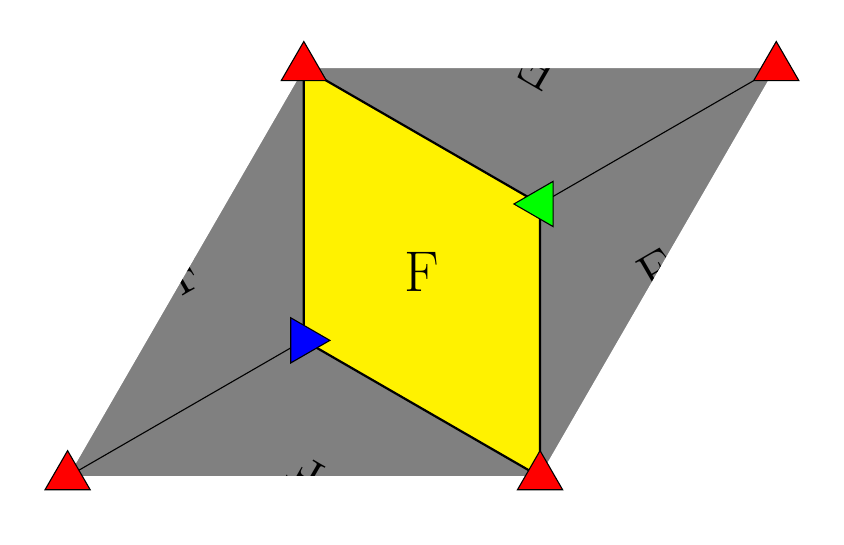
\begin{tikzpicture}
            % Define the lengths of the sides and the angle
            \def\a{3}  % length of side a
            \def\b{3}  % length of side b
            \def\angle{60}  % angle between sides a and b
            \def\s{F} % Label in center of cells

            \def\x{0.5} % Boundary 
            \def\y{0.5} % Boundary

        
            % Calculate the coordinates of the points
            \coordinate (C00) at (0, 0);
            \coordinate (C10) at (\a, 0);
            \coordinate (C11) at ({\a + \b*cos(\angle)}, {\b * sin(\angle)});
            \coordinate (C01) at ({\b * cos(\angle)}, {\b * sin(\angle)});
            \coordinate (C02) at ({2*\b*cos(\angle)}, {2*\b * sin(\angle)});
            \coordinate (C12) at ({\a +2*\b * cos(\angle)}, {2*\b * sin(\angle)});
            \coordinate (C22) at ({2*\a + 2*\b * cos(\angle)}, {2*\b * sin(\angle)});
            \coordinate (C21) at ({2*\a + \b*cos(\angle)}, {\b * sin(\angle)});
            \coordinate (C20) at ({2*\a}, 0);
        
            % Draw the oblique unit cell
            \draw[fill=gray,gray] (C00) -- (C20) -- (C22) -- (C02) -- cycle;
            \draw[thick,fill=yellow] ($(C00)!0.6666!(C11)$) -- (C20) -- ($(C11)!0.3333!(C22)$) -- (C02) -- cycle;

            
            % Draw boundary chiral centres
            \node[rotate=150] at (C10) {\huge \s};
            \node[rotate=30] at (C21) {\huge \s};
            \node[rotate=150] at (C12) {\huge \s};
            \node[rotate=30] at (C01) {\huge \s};

            % Create white border
            \draw[fill=white,white] ($(C00)-(\x,\y)$) -- ($(C20)-(-\x,\y)$) -- (C20) -- (C00);
            \draw[fill=white,white] ($(C00)-(\x,-\y)$) -- ($(C02)-(\x,-\y)$) -- (C02) -- (C00);
            \draw[fill=white,white] ($(C02)+(\x,\y)$) -- ($(C22)-(\x,-\y)$) -- (C22) -- (C02);
            \draw[fill=white,white] ($(C20)+(\x,-\y)$) -- ($(C22)+(\x,\y)$) -- (C22) -- (C20);

            % Draw chiral inner centre
            \node at (C11) {\huge \s};


            % Draw mirrow lines
            \draw (C00) -- ($(C00)!0.6666!(C11)$);
            \draw ($(C11)!0.3333!(C22)$) -- (C22);


            % Draw node reflections
            \draw (C00)  node[regular polygon, regular polygon sides=3, draw, fill=red, minimum size=0.5cm] {};
            \draw (C02)  node[regular polygon, regular polygon sides=3, draw, fill=red, minimum size=0.5cm] {};
            \draw (C22)  node[regular polygon, regular polygon sides=3, draw, fill=red, minimum size=0.5cm] {};
            \draw (C20)  node[regular polygon, regular polygon sides=3, draw, fill=red, minimum size=0.5cm] {};

            \draw ($(C00)!0.6666!(C11)$)  node[rotate = 30,regular polygon, regular polygon sides=3, draw, fill=blue, minimum size=0.5cm] {};
            \draw ($(C11)!0.3333!(C22)$)  node[rotate=90, regular polygon, regular polygon sides=3, draw, fill=green, minimum size=0.5cm] {};    
        \end{tikzpicture}
\end{document}
        \caption{p3 cell diagram.}
        \label{fig:enter-label}
    \end{figure}
\end{frame}
\begin{frame}{p31m cell diagram}
    \begin{figure}
        \centering
        \documentclass[class=article, crop=false]{standalone}
\usepackage{tikz}
\usepackage{subcaption}
\usetikzlibrary{calc}
\usetikzlibrary {shapes.geometric}

\begin{document}
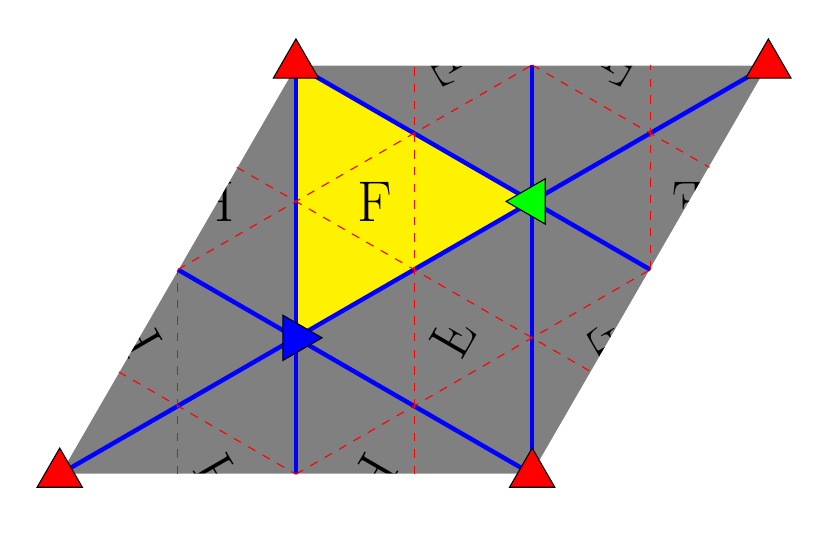
\begin{tikzpicture}
            % Define the lengths of the sides and the angle
            \def\a{3}  % length of side a
            \def\b{3}  % length of side b
            \def\angle{60}  % angle between sides a and b
            \def\s{F} % Label in center of cells

            \def\x{0.4}
            \def\y{0.4}
        
            % Calculate the coordinates of the points
            \coordinate (C00) at (0, 0);
            \coordinate (C10) at (\a, 0);
            \coordinate (C11) at ({\a + \b*cos(\angle)}, {\b * sin(\angle)});
            \coordinate (C01) at ({\b * cos(\angle)}, {\b * sin(\angle)});
            \coordinate (C02) at ({2*\b*cos(\angle)}, {2*\b * sin(\angle)});
            \coordinate (C12) at ({\a +2*\b * cos(\angle)}, {2*\b * sin(\angle)});
            \coordinate (C22) at ({2*\a + 2*\b * cos(\angle)}, {2*\b * sin(\angle)});
            \coordinate (C21) at ({2*\a + \b*cos(\angle)}, {\b * sin(\angle)});
            \coordinate (C20) at ({2*\a}, 0);
            \coordinate (A1) at ($(C00)!0.6666!(C11)$);
            \coordinate (A2) at ($(C11)!0.3333!(C22)$);
        

            % Draw the oblique unit cell
            \draw[thick,fill=gray,gray] (C00) -- (C20) -- (C22) -- (C02) -- cycle;
            \draw[thick,fill=yellow,yellow] (A1) -- (A2) -- (C02) -- cycle;
            %\draw[thick] (C10) -- (C21) -- (C12) -- (C01) -- cycle;
            

            % Draw bourdary chiral centres
            \node[rotate=240] at ($(C10)!0.3333!(C20)$) {\huge \s};
            \node[rotate=120] at ($(C00)!0.6666!(C10)$) {\reflectbox{\huge \s}};
            \node[rotate=120] at ($(C00)!0.6666!(C01)$) {\huge \s};
            \node at ($(C01)!0.3333!(C02)$) {\reflectbox{\huge \s}};
            \node[rotate=120] at ($(C02)!0.6666!(C12)$) {\reflectbox{\huge \s}};
            \node[rotate=240] at ($(C12)!0.3333!(C22)$) {\huge \s};
            \node[rotate=120] at ($(C20)!0.6666!(C21)$) {\huge \s};
            \node at ($(C21)!0.3333!(C22)$) {\reflectbox{\huge \s}};

            % Create white border
            \draw[fill=white,white] ($(C00)-(\x,\y)$) -- ($(C20)-(-\x,\y)$) -- (C20) -- (C00);
            \draw[fill=white,white] ($(C00)-(\x,-\y)$) -- ($(C02)-(\x,-\y)$) -- (C02) -- (C00);
            \draw[fill=white,white] ($(C02)+(\x,\y)$) -- ($(C22)-(\x,-\y)$) -- (C22) -- (C02);
            \draw[fill=white,white] ($(C20)+(\x,-\y)$) -- ($(C22)+(\x,\y)$) -- (C22) -- (C20);

            % Draw inner chiral centres
            \node at ($(A1)!0.5!(A2)!0.3333!(C02)$) {\huge \s};
            \node[rotate=240] at ($(A1)!0.5!(A2)!0.3333!(C20)$) {\reflectbox{\huge \s}};

        

            % Draw mirrow lines
            \draw[ultra thick,blue] (C00)--(C22);
            \draw[ultra thick,blue] (C01)--(C20);
            \draw[ultra thick,blue] (C10)--(C02);
            \draw[ultra thick,blue] (C12)--(C20);
            \draw[ultra thick,blue] (C02)--(C21);
            \draw[dashed,red] ($(C00)!0.5!(C10)$)--(C01);
            \draw[dashed,red] ($(C00)!0.5!(C01)$)--(C10);
            \draw[dashed,red] ($(C10)!0.5!(C20)$)--($(C02)!0.5!(C12)$);
            \draw[dashed,red] ($(C01)!0.5!(C02)$)--($(C20)!0.5!(C21)$);
            \draw[dashed,red] (C01)--(C12);
            \draw[dashed,red] (C10)--(C21);
            \draw[dashed,red] (C12)--($(C21)!0.5!(C22)$);
            \draw[dashed,red] (C21)--($(C12)!0.5!(C22)$);
            

            

            % Draw node reflections
            \draw (C00)  node[regular polygon, regular polygon sides=3, draw, fill=red, minimum size=0.5cm] {};
            %\draw (C10)  node[shape aspect=0.5,rotate=90,diamond,draw,fill=blue] {};
            %\draw (C11)  node[shape aspect=0.5,diamond,draw,fill=red] {};
            %\draw (C01)  node[shape aspect=0.5,rotate=90,diamond,draw,fill=blue] {};
            \draw (C02)  node[regular polygon, regular polygon sides=3, draw, fill=red, minimum size=0.5cm] {};
            %\draw (C12)  node[shape aspect=0.5,rotate=90,diamond,draw,fill=blue] {};
            \draw (C22)  node[regular polygon, regular polygon sides=3, draw, fill=red, minimum size=0.5cm] {};
            %\draw (C21)  node[shape aspect=0.5,rotate=90,diamond,draw,fill=blue] {};
            \draw (C20)  node[regular polygon, regular polygon sides=3, draw, fill=red, minimum size=0.5cm] {};

            \draw (A1)  node[rotate = 30,regular polygon, regular polygon sides=3, draw, fill=blue, minimum size=0.5cm] {};
            \draw (A2)  node[rotate=90, regular polygon, regular polygon sides=3, draw, fill=green, minimum size=0.5cm] {};

            %\draw ($(A)!0.5!(E)$) node[shape aspect=0.5,diamond,draw,fill=black] {};
            
        \end{tikzpicture}
\end{document}
        \caption{p31m cell diagram.}
        \label{fig:enter-label}
    \end{figure}
\end{frame}
\begin{frame}{p3m1 cell diagram}
    \begin{figure}
        \centering
        \documentclass[class=article, crop=false]{standalone}
\usepackage{tikz}
\usepackage{subcaption}
\usetikzlibrary{calc}
\usetikzlibrary {shapes.geometric}

\begin{document}
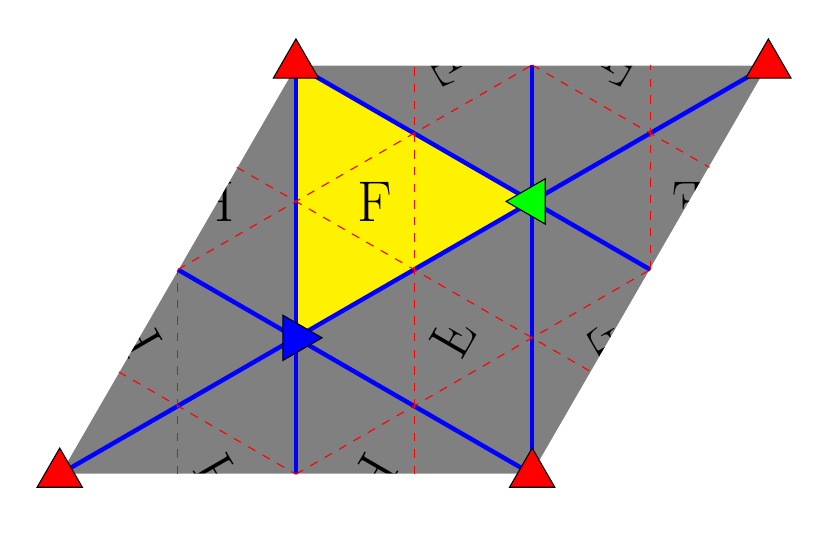
\begin{tikzpicture}
            % Define the lengths of the sides and the angle
            \def\a{3}  % length of side a
            \def\b{3}  % length of side b
            \def\angle{60}  % angle between sides a and b
            \def\s{F} % Label in center of cells

            \def\x{0.4}
            \def\y{0.4}
        
            % Calculate the coordinates of the points
            \coordinate (C00) at (0, 0);
            \coordinate (C10) at (\a, 0);
            \coordinate (C11) at ({\a + \b*cos(\angle)}, {\b * sin(\angle)});
            \coordinate (C01) at ({\b * cos(\angle)}, {\b * sin(\angle)});
            \coordinate (C02) at ({2*\b*cos(\angle)}, {2*\b * sin(\angle)});
            \coordinate (C12) at ({\a +2*\b * cos(\angle)}, {2*\b * sin(\angle)});
            \coordinate (C22) at ({2*\a + 2*\b * cos(\angle)}, {2*\b * sin(\angle)});
            \coordinate (C21) at ({2*\a + \b*cos(\angle)}, {\b * sin(\angle)});
            \coordinate (C20) at ({2*\a}, 0);
            \coordinate (A1) at ($(C00)!0.6666!(C11)$);
            \coordinate (A2) at ($(C11)!0.3333!(C22)$);
        

            % Draw the oblique unit cell
            \draw[thick,fill=gray,gray] (C00) -- (C20) -- (C22) -- (C02) -- cycle;
            \draw[thick,fill=yellow,yellow] (A1) -- (A2) -- (C02) -- cycle;
            %\draw[thick] (C10) -- (C21) -- (C12) -- (C01) -- cycle;
            

            % Draw bourdary chiral centres
            \node[rotate=240] at ($(C10)!0.3333!(C20)$) {\huge \s};
            \node[rotate=120] at ($(C00)!0.6666!(C10)$) {\reflectbox{\huge \s}};
            \node[rotate=120] at ($(C00)!0.6666!(C01)$) {\huge \s};
            \node at ($(C01)!0.3333!(C02)$) {\reflectbox{\huge \s}};
            \node[rotate=120] at ($(C02)!0.6666!(C12)$) {\reflectbox{\huge \s}};
            \node[rotate=240] at ($(C12)!0.3333!(C22)$) {\huge \s};
            \node[rotate=120] at ($(C20)!0.6666!(C21)$) {\huge \s};
            \node at ($(C21)!0.3333!(C22)$) {\reflectbox{\huge \s}};

            % Create white border
            \draw[fill=white,white] ($(C00)-(\x,\y)$) -- ($(C20)-(-\x,\y)$) -- (C20) -- (C00);
            \draw[fill=white,white] ($(C00)-(\x,-\y)$) -- ($(C02)-(\x,-\y)$) -- (C02) -- (C00);
            \draw[fill=white,white] ($(C02)+(\x,\y)$) -- ($(C22)-(\x,-\y)$) -- (C22) -- (C02);
            \draw[fill=white,white] ($(C20)+(\x,-\y)$) -- ($(C22)+(\x,\y)$) -- (C22) -- (C20);

            % Draw inner chiral centres
            \node at ($(A1)!0.5!(A2)!0.3333!(C02)$) {\huge \s};
            \node[rotate=240] at ($(A1)!0.5!(A2)!0.3333!(C20)$) {\reflectbox{\huge \s}};

        

            % Draw mirrow lines
            \draw[ultra thick,blue] (C00)--(C22);
            \draw[ultra thick,blue] (C01)--(C20);
            \draw[ultra thick,blue] (C10)--(C02);
            \draw[ultra thick,blue] (C12)--(C20);
            \draw[ultra thick,blue] (C02)--(C21);
            \draw[dashed,red] ($(C00)!0.5!(C10)$)--(C01);
            \draw[dashed,red] ($(C00)!0.5!(C01)$)--(C10);
            \draw[dashed,red] ($(C10)!0.5!(C20)$)--($(C02)!0.5!(C12)$);
            \draw[dashed,red] ($(C01)!0.5!(C02)$)--($(C20)!0.5!(C21)$);
            \draw[dashed,red] (C01)--(C12);
            \draw[dashed,red] (C10)--(C21);
            \draw[dashed,red] (C12)--($(C21)!0.5!(C22)$);
            \draw[dashed,red] (C21)--($(C12)!0.5!(C22)$);
            

            

            % Draw node reflections
            \draw (C00)  node[regular polygon, regular polygon sides=3, draw, fill=red, minimum size=0.5cm] {};
            %\draw (C10)  node[shape aspect=0.5,rotate=90,diamond,draw,fill=blue] {};
            %\draw (C11)  node[shape aspect=0.5,diamond,draw,fill=red] {};
            %\draw (C01)  node[shape aspect=0.5,rotate=90,diamond,draw,fill=blue] {};
            \draw (C02)  node[regular polygon, regular polygon sides=3, draw, fill=red, minimum size=0.5cm] {};
            %\draw (C12)  node[shape aspect=0.5,rotate=90,diamond,draw,fill=blue] {};
            \draw (C22)  node[regular polygon, regular polygon sides=3, draw, fill=red, minimum size=0.5cm] {};
            %\draw (C21)  node[shape aspect=0.5,rotate=90,diamond,draw,fill=blue] {};
            \draw (C20)  node[regular polygon, regular polygon sides=3, draw, fill=red, minimum size=0.5cm] {};

            \draw (A1)  node[rotate = 30,regular polygon, regular polygon sides=3, draw, fill=blue, minimum size=0.5cm] {};
            \draw (A2)  node[rotate=90, regular polygon, regular polygon sides=3, draw, fill=green, minimum size=0.5cm] {};

            %\draw ($(A)!0.5!(E)$) node[shape aspect=0.5,diamond,draw,fill=black] {};
            
        \end{tikzpicture}
\end{document}
        \caption{p3m1 cell diagram.}
        \label{fig:enter-label}
    \end{figure}
\end{frame}
\begin{frame}{p6 cell diagram}
    \begin{figure}
        \centering
        \documentclass[class=article, crop=false]{standalone}
\usepackage{tikz}
\usepackage{subcaption}
\usetikzlibrary{calc}
\usetikzlibrary {shapes.geometric}

\begin{document}
\begin{tikzpicture}
            % Define the lengths of the sides and the angle
            \def\a{3}  % length of side a
            \def\b{3}  % length of side b
            \def\angle{60}  % angle between sides a and b
            \def\s{F} % Label in center of cells
        
            % Calculate the coordinates of the points
            \coordinate (C00) at (0, 0);
            \coordinate (C10) at (\a, 0);
            \coordinate (C11) at ({\a + \b*cos(\angle)}, {\b * sin(\angle)});
            \coordinate (C01) at ({\b * cos(\angle)}, {\b * sin(\angle)});
            \coordinate (C02) at ({2*\b*cos(\angle)}, {2*\b * sin(\angle)});
            \coordinate (C12) at ({\a +2*\b * cos(\angle)}, {2*\b * sin(\angle)});
            \coordinate (C22) at ({2*\a + 2*\b * cos(\angle)}, {2*\b * sin(\angle)});
            \coordinate (C21) at ({2*\a + \b*cos(\angle)}, {\b * sin(\angle)});
            \coordinate (C20) at ({2*\a}, 0);

            \coordinate (A1) at ($(C00)!0.6666!(C11)$);
            \coordinate (A2) at ($(C11)!0.3333!(C22)$);
        
            % Draw the oblique unit cell
            \draw[thick,fill=gray] (C00) -- (C20) -- (C22) -- (C02) -- cycle;
            \draw[thick,fill=yellow] (C00) -- (A1) -- (C20) -- cycle;
            %\draw[thick] (C10) -- (C21) -- (C12) -- (C01) -- cycle;
            
            % Draw mirrow lines
            \draw[thin] (C02) -- (A1);
            \draw[thin] (C02) -- (C11) -- (C20);
            \draw[thin] (C02) -- (A2) -- (C20);
            \draw[thin] (A2) -- (C22);
            
            % Draw chiral center
            $\node at ($(C00)!0.5!(C20)!0.5!(A1)$) {\huge \s};
            \node[rotate=240] at ($(C00)!0.5!(C02)!0.5!(A1)$) {\huge \s};
            \node[rotate=120] at ($(C20)!0.5!(C02)!0.5!(A1)$) {\huge \s};
            \node[rotate=300] at ($(C20)!0.5!(C02)!0.5!(A2)$) {\huge \s};
            \node[rotate=60] at ($(C22)!0.5!(C20)!0.5!(A2)$) {\huge \s};
            \node[rotate=180] at ($(C02)!0.5!(C22)!0.5!(A2)$) {\huge \s};

            % Draw node rotations
            \draw (C00)  node[regular polygon, regular polygon sides=6, draw, fill=blue, minimum size=0.5cm] {};
            \draw (C10)  node[shape aspect=0.5,diamond,draw,fill=black] {};
            \draw (C21)  node[shape aspect=0.5,diamond,draw,fill=black] {};
            \draw (C01)  node[shape aspect=0.5,diamond,draw,fill=black] {};
            \draw (C12)  node[shape aspect=0.5,diamond,draw,fill=black] {};
            \draw (C02)  node[regular polygon, regular polygon sides=6, draw, fill=blue, minimum size=0.5cm] {};
            %\draw (C12)  node[shape aspect=0.5,rotate=90,diamond,draw,fill=blue] {};
            \draw (C22)  node[regular polygon, regular polygon sides=6, draw, fill=blue, minimum size=0.5cm] {};
            %\draw (C21)  node[shape aspect=0.5,rotate=90,diamond,draw,fill=blue] {};
            \draw (C20)  node[regular polygon, regular polygon sides=6, draw, fill=blue, minimum size=0.5cm] {};

            \draw (A1)  node[regular polygon, regular polygon sides=3, draw, fill=red, minimum size=0.5cm] {};
            \draw (A2)  node[regular polygon, regular polygon sides=3, draw, fill=red, minimum size=0.5cm] {};

            \draw (C11) node[shape aspect=0.5,diamond,draw,fill=black] {};
            
        \end{tikzpicture}
\end{document}
        \caption{p6 cell diagram.}
        \label{fig:enter-label}
    \end{figure}
\end{frame}
\begin{frame}{p6m cell diagram}
    \begin{figure}
        \centering
        \documentclass[class=article, crop=false]{standalone}
\usepackage{tikz}
\usepackage{subcaption}
\usetikzlibrary{calc}
\usetikzlibrary {shapes.geometric}

\begin{document}
\begin{tikzpicture}
    % Define the lengths of the sides and the angle
    \def\a{3}  % length of side a
    \def\b{3}  % length of side b
    \def\angle{60}  % angle between sides a and b
    \def\s{T} % Label in center of cells

    % Calculate the coordinates of the points
    \coordinate (C00) at (0, 0);
g10) at (\a, 0);
    \coordinate (C11) at ({\a + \b*cos(\angle)}, {\b * sin(\angle)});
    \coordinate (C01) at ({\b * cos(\angle)}, {\b * sin(\angle)});
    \coordinate (C02) at ({2*\b*cos(\angle)}, {2*\b * sin(\angle)});
    \coordinate (C12) at ({\a +2*\b * cos(\angle)}, {2*\b * sin(\angle)});
    \coordinate (C22) at ({2*\a + 2*\b * cos(\angle)}, {2*\b * sin(\angle)});
    \coordinate (C21) at ({2*\a + \b*cos(\angle)}, {\b * sin(\angle)});
    \coordinate (C20) at ({2*\a}, 0);

    \coordinate (A1) at ($(C00)!0.6666!(C11)$);
    \coordinate (A2) at ($(C11)!0.3333!(C22)$);

    % Draw the oblique unit cell
    \draw[fill=gray] (C00) -- (C20) -- (C22) -- (C02) -- cycle;
    \draw[thick,fill=yellow] (C00) -- (C10) -- ($(C00)!0.6666!(C11)$) -- cycle;
    \draw[ultra thick,pink] (C00) -- (C20) -- (C22) -- (C02) -- cycle;
    \draw[ultra thick,pink] (C20) -- (C02);
    \draw[ultra thick,blue] (C00) -- (C22);
    \draw[ultra thick,blue] (C01) -- (C20);
    \draw[ultra thick,blue] (C10) -- (C02);
    \draw[ultra thick,blue] (C02) -- (C21);
    \draw[ultra thick,blue] (C20) -- (C12);
    
    % Draw mirrow lines
    \draw[dashed,blue] ($(C01)!0.5!(C02)$) -- ($(C20)!0.5!(C21)$);
    \draw[dashed,blue] ($(C10)!0.5!(C20)$) -- ($(C02)!0.5!(C12)$);
    \draw[dashed] (C01) -- (C21);
    \draw[dashed] (C10) -- (C12);
    \draw[dashed,red] (C01) -- (C12);
    \draw[dashed,red] (C10) -- (C21);
    \draw[dashed,red] (C01) -- (C10);
    \draw[dashed,red] (C21) -- (C12);
    \draw[dashed,red] (C01) -- ($(C00)!0.5!(C10)$);
    \draw[dashed,red] (C10) -- ($(C00)!0.5!(C01)$);
    \draw[dashed,red] (C21) -- ($(C12)!0.5!(C22)$);
    \draw[dashed,red] (C12) -- ($(C21)!0.5!(C22)$);
    
    % Draw chiral center
    \node at ($(C00)!0.5!(C10)!0.3333!(A1)$) {\huge \s};
    \node[rotate=240] at ($(C00)!0.5!(A1)!0.3333!(C01)$) {\reflectbox{\huge\s}};
    \node[rotate=0] at ($(C10)!0.5!(A1)!0.3333!(C20)$) {\reflectbox{\huge \s}};
    \node[rotate=120] at ($(A1)!0.5!(C11)!0.3333!(C20)$) {\huge \s};
    \node[rotate=300] at ($(C11)!0.5!(A2)!0.3333!(C20)$) {\reflectbox{\huge \s}};
    \node[rotate=60] at ($(C21)!0.5!(A2)!0.3333!(C20)$) {\huge \s};
    \node[rotate=60] at ($(C21)!0.5!(A2)!0.3333!(C22)$) {\reflectbox{\huge \s}};
    \node[rotate=180] at ($(C12)!0.5!(A2)!0.3333!(C22)$) {\huge \s};
    \node[rotate=300] at ($(C11)!0.5!(A2)!0.3333!(C02)$) {\huge \s};
    \node[rotate=180] at ($(C12)!0.5!(A2)!0.3333!(C02)$) {\reflectbox{\huge \s}};
    \node[rotate=240] at ($(C01)!0.5!(A1)!0.3333!(C02)$) {\huge \s};
    \node[rotate=120] at ($(C11)!0.5!(A1)!0.3333!(C02)$) {\reflectbox{\huge \s}};

    % Draw node reflections
    \draw (C00)  node[regular polygon, regular polygon sides=6, draw, fill=blue, minimum size=0.5cm] {};
    \draw (C10)  node[shape aspect=0.5, diamond,draw,fill=pink] {};
    \draw (C11)  node[shape aspect=0.5,diamond,draw,fill=pink] {};
    \draw (C01)  node[shape aspect=0.5,diamond,draw,fill=pink] {};
    \draw (C02)  node[regular polygon, regular polygon sides=6, draw, fill=blue, minimum size=0.5cm] {};
    \draw (C12)  node[shape aspect=0.5,diamond,draw,fill=pink] {};
    \draw (C22)  node[regular polygon, regular polygon sides=6, draw, fill=blue, minimum size=0.5cm] {};
    \draw (C21)  node[shape aspect=0.5,diamond,draw,fill=pink] {};
    \draw (C20)  node[regular polygon, regular polygon sides=6, draw, fill=blue, minimum size=0.5cm] {};

    \draw (A1)  node[regular polygon, regular polygon sides=3, draw, fill=red, minimum size=0.5cm] {};
    \draw (A2)  node[regular polygon, regular polygon sides=3, draw, fill=red, minimum size=0.5cm] {};
\end{tikzpicture}
\end{document}
        \caption{p6m cell diagram.}
        \label{fig:enter-label}
    \end{figure}
\end{frame}
\end{document}